
\part{Beobachterentwurf\label{part:Beobachterentwurf}}

\chapter{Beobachter mit großer Verstärkung und starke Beobachter\label{chap:High-Gain-Beobachter}}

Die in den Kapiteln~\ref{chap:regler-grundlagen} und~\ref{chap:regler-varianten}
entworfenen Rückführungen setzen in der Regel die Kenntnis des vollständigen
Systemzustands voraus. In der regelungstechnischen Praxis wird dagegen
meist nur ein Teil der Zustände messtechnisch erfasst. Dieses Kapitel
behandelt einige Ansätze für Zustandsbeobachter, mit denen aus aktuellen
Messdaten von Eingang und Ausgang der jeweilige Systemzustand asymptotisch
rekonstruiert wird. Der Hauptteil des Kapitels befasst sich mit Beobachtern,
bei denen die im System auftretenden Nichtlinearitäten durch eine
lineare Aufschaltung dominiert werden. Zusätzlich wird auf starke
Beobachter eingegangen, welche den Zustand ohne Kenntnis des Systemeingangs
schätzen.

\section{Beobachterentwurf in Originalkoordinaten}

Gegeben sei ein nichtlineares System
\begin{equation}
\dot{x}=F(x,u),\quad y=h(x)\label{eq:hg-system-nicht-affin}
\end{equation}
mit einem eingangsabhängigen Vektorfeld $F:\mathcal{M}\times\mathcal{U}\to\R^{n}$,
der offenen Menge $\mathcal{M}\subseteq\R^{n}$ und dem zulässigen
Wertebereich $\mathcal{U}\subseteq\R^{m}$ der Eingangs\-signale.
Die auf der Menge~$\mathcal{M}$ definierte Abbildung~$h$ überführt
den Zustand~$x$ in die Ausgangsgröße~$y$. Wir gehen davon aus,
dass die Zeitverläufe des Eingangs~$u$ und des Ausgangs~$y$ gemessen
werden. Die Regelung von System~(\ref{eq:hg-system-nicht-affin})
mittels Zustandsrückführung erfordert die Kenntnis des Zustands~$x$.
Da der Ausgang in der Regel eine niedrigere Dimension besitzt als
der Zustand, d.\,h. $\dim y<\dim x$, lässt sich der Zustand~$x$
nicht eindeutig durch eine Umkehrung der Abbildung~$h$ ermitteln.
Stattdessen entwirft man in Ergänzung zu der gegebenen Regelstrecke~(\ref{eq:hg-system-nicht-affin})
ein weiteres dynamisches System, den sogenannten \emph{Beobachter}\index{Beobachter}
bzw. \emph{Zustandsbeobachter} (engl. \emph{state observer}), mit
der allgemeinen Struktur
\begin{equation}
\dot{\hat{z}}=\hat{F}(\hat{z},u,y),\quad\hat{x}=\hat{H}(\hat{z},u,y).\label{eq:hg-beobachter-allgemein}
\end{equation}
Abb.~\ref{fig:beobachter-struktur} skizziert die Verknüpfung von
System und Beobachter. Der Beobachter~(\ref{eq:hg-beobachter-allgemein})
ist so zu entwerfen, dass (ggf. unter zusätzlichen Voraussetzungen
an die Anfangswerte) der geschätzte Zustand~$\hat{x}(t)$ gegen den
Systemzustand~$x(t)$ für $t\to\infty$ konvergiert. In Abhängigkeit
von der Dimension des Zustandsraums des Beobachters~(\ref{eq:hg-beobachter-allgemein})
unterscheidet man zwischen einem \emph{Identitätsbeobachter} ($\dim\hat{z}=\dim x$,
insbesondere $\hat{z}=\hat{x}$), einem \emph{reduzierten Beobachter}\index{Beobachter!reduzierter}
($\dim\hat{z}<\dim x$) sowie einem \emph{Einbettungsbeobachter}\index{Beobachter!Einbettungs-}
($\dim\hat{z}>\dim x$).

Dieser Abschnitt widmet sich dem Entwurf von Beobachtern in den Originalkoordinaten
des Systems. Das dabei entwickelte Entwurfskonzept von Beobachtern
mit großer Verstärkung wird in den Abschnitten~\ref{sec:High-Gain-Entwurf-Beobachtbarkeitsnormalform}
und~\ref{sec:High-Gain-Entwurf-Eingangs-Ausgangs-Normalform} auf
den Beobachterentwurf in den Koordinaten verschiedener Normalformen
übertragen.

\begin{figure}
\begin{centering}
\resizebox{0.6\textwidth}{!}{
\chapter[Beobachterentwurf mittels  Linearisierung der Fehlerdynamik]{Beobachterentwurf mittels exakter bzw. näherungsweiser Linearisierung
der Fehlerdynamik\label{cha:Beobachter-Normalform}}

Normalformen spielen beim Entwurf nichtlinearer Beobachter eine große
Rolle. Kann man ein System in eine Form überführen, bei der die Nichtlinearitäten
ausschließlich von den Messgrößen abhängen, ist der Entwurf eines
Beobachters mit exakt linearer Fehlerdynamik vergleichsweise einfach.
Eine solche Form ist die Beobachternormalform. Die Transformation
in diese Form und damit verbunden die Linearisierung des Beobachtungsfehlers
ist aufgrund restriktiver Existenzbedingungen bzw. einer aufwendigen
Berechnung in der regelungstechnischen Praxis kaum anzutreffen. Bei
genauerer Betrachtung eröffnen sich jedoch etliche Möglichkeiten zur
Berechnung bzw. zur Approximation eines Beobachters mit linearer Fehlerdynamik.
In diesem Kapitel werden Existenzbedingungen und Berechnungsmethoden
vorgestellt.\footnote{Das Kapitel basiert sich an dem Übersichtsbeitrag Röbenack, K.: Entwurf
nichtlinear Beobachter mit linearer und näherungsweise linearer Fehlerdynamik,
Automatisierungstechnik, De Gruyter-Verlag, Berlin, Boston, Jahrgang~58,
Heft~9, S.~489-497, für den der De~Gruyter-Verlag freundlicherweise
eine Nutzungsgenehmigung erteilt hat.}

\section{Linearisierung des Beobachtungsfehlers durch Aufschaltung\label{sec:Linearisierung-durch-Aufschaltung}}

In diesem Abschnitt soll zunächst die grundsätzliche Idee der exakten
Linearisierung des Beobachtungsfehlers durch Aufschaltung illustriert
werden. Angenommen, das zu beobachtende System kann in der Form
\begin{equation}
\dot{x}=Ax+\alpha(y,u),\quad y=c^{T}x\label{eq:lin-beob-fehler-strecke}
\end{equation}
mit dem Zustand~$x$, dem Eingang~$u$, und dem gemessenen Ausgang~$y$
dargestellt werden. Dabei sei der durch das Paar $(A,c^{T})$ beschriebene
lineare Teil beobachtbar. Zusätzlich seien alle auftretenden Nichtlinearitäten
in Abhängigkeit vom Ausgang darstellbar. Diese Nichtlinearitäten werden
in der Eingangs-Ausgangs-Aufschaltung~$\alpha$ zusammengefasst.
Setzt man den Beobachter in der Form
\begin{equation}
\dot{\hat{x}}=A\hat{x}+\alpha(y,u)+l\cdot\left(y-c^{T}\hat{x}\right)\label{eq:lin-beob-fehler-beobachter}
\end{equation}
mit einer Beobachterverstärkung $l\in\R^{n}$ an. so genügt der Beobachtungsfehler
$\tilde{x}=x-\hat{x}$ der linearen zeitinvarianten Differentialgleichung
\begin{equation}
\begin{array}{lcl}
\dot{\tilde{x}} & = & \dot{x}-\dot{\hat{x}}\\
 & = & Ax+\alpha(y,u)-A\hat{x}-\alpha(y,u)-l\cdot\left(y-c^{T}\hat{x}\right)\\
 & = & \left(A-lc^{T}\right)\tilde{x}.
\end{array}\label{eq:lin-beob-fehler-dynamik}
\end{equation}
Über die Verstärkung~$l$ kann man für die Systemmatrix $A-lc^{T}$
der Fehlerdynamik~(\ref{eq:lin-beob-fehler-dynamik}) ein beliebiges
charakteristisches Polynom

\begin{equation}
\det(sI-A+lc^{T})=a_{0}+a_{1}s+\cdots+a_{n-1}s^{n-1}+s^{n}\label{eq:cp}
\end{equation}
vorgeben. Diese Herangehensweise soll an zwei Beispielen vorgestellt
werden:

\begin{example}
\label{exa:inverses-pendel-motor-nf-beobachter}Wir betrachten das
Modell des inversen Pendels mit Gleich\-strom\-antrieb aus Beispiel~\ref{exa:inverses-pendel-gleichstrommotor}:

\begin{equation}
\begin{array}{lcl}
\dot{x}_{1} & = & x_{2}\\
\dot{x}_{2} & = & \frac{mg\ell}{J}\sin x_{1}-\frac{d}{J}x_{2}+\frac{K}{J}x_{3}\\
\dot{x}_{3} & = & -\frac{K}{L}x_{2}-\frac{R}{L}x_{3}+\frac{1}{L}u\\
y & = & x_{1}.
\end{array}\label{eq:inverses-pendel-motor-nf-strecke}
\end{equation}
Als Messgröße steht der Winkel~$x_{1}$, der beispielsweise mit einem
Inkrementgeber erfasst werden kann, zur Verfügung. Die einzige im
System auftretende Nichtlinearität hängt ausschließlich vom Ausgang~$x_{1}$
ab. Der Beobachter setzt sich dann aus einer Kopie des Systems, wobei
die Nichtlinearität vom gemessenen Ausgang gespeist wird, und einem
linearen Korrekturterm zusammen: 
\begin{equation}
\left(\begin{array}{l}
\dot{\hat{x}}_{1}\\
\dot{\hat{x}}_{2}\\
\dot{\hat{x}}_{3}
\end{array}\right)=\left(\begin{array}{c}
\hat{x}_{2}\\
\frac{mg\ell}{J}\sin y-\frac{d}{J}\hat{x}_{2}+\frac{K}{J}\hat{x}_{3}\\
-\frac{K}{L}\hat{x}_{2}-\frac{R}{L}\hat{x}_{3}+\frac{1}{L}u
\end{array}\right)+\left(\begin{array}{l}
l_{1}\\
l_{2}\\
l_{3}
\end{array}\right)\cdot\left(y-\hat{x}_{1}\right)\label{eq:inverses-pendel-motor-nf-beobachter}
\end{equation}
Der Vergleich von~(\ref{eq:inverses-pendel-motor-nf-strecke}) und~(\ref{eq:inverses-pendel-motor-nf-beobachter})
führt auf eine lineare Fehlerdynamik~(\ref{eq:lin-beob-fehler-dynamik}).
Für ein vorgegebenes charakteristisches Polynom~(\ref{eq:cp}) mit
den Koeffizienten $a_{0},a_{1},a_{2}>0$ berechnet man durch Koeffizientenvergleich
oder mit Hilfe der Ackermann-Formel~\cite{acker77,ackermann77} die
Beobachterverstärkung 
\begin{equation}
\begin{array}{lcl}
l_{1} & = & -\frac{R}{L}-\frac{d}{J}+a_{2},\\
l_{2} & = & \frac{-JK^{2}L+\left(a_{1}J^{2}-a_{2}dJ+d^{2}\right)L^{2}-J\left(a_{2}J-d\right)LR+J^{2}R^{2}}{J^{2}L^{2}},\\
l_{3} & = & -\frac{\left(a_{2}J-d\right)K^{2}L^{2}-a_{0}J^{2}L^{3}+JL\left(a_{1}JL-2K^{2}\right)R-a_{2}J^{2}LR^{2}+J^{2}R^{3}}{JKL^{3}}.
\end{array}\label{eq:inverses-pendel-motor-nf-verstaerkung}
\end{equation}
\end{example}

\begin{example}
\label{exa:inverses-pendel-elastisch}Wir betrachten wiederum einen
Manipulator in der Form eines inversen Pendels (siehe Abb.~\ref{fig:Inverses-Pendel-elastisch}).
Der Antrieb erfolgt über ein eingeprägtes Drehmoment~$u$, welches
den Winkel~$q_{1}$ beeinflusst. Der Antrieb ist über eine elastische
Welle, die als Torsionsfeder mit der Federkonstanten~$k$ modelliert
wird, mit dem Manipulatorarm verbunden. Die Position des Manipulatorarms
wird durch den Relativwinkel~$q_{2}$ beschrieben. Der Manipulator
habe beim Antrieb das Trägheitsmoment~$J_{1}$ und hinsichtlich des
Manipulatorarms das Trägheitsmoment~$J_{2}$. Am Ende des Manipulatorarms
der Länge~$\ell$ befinde sich eine Last mit der Masse~$m$.

Das System hat die kinetische Energie
\[
T=\frac{J_{1}}{2}\dot{q}_{1}^{2}+\frac{J_{2}}{2}\left(\dot{q}_{1}+\dot{q}_{2}\right)^{2}
\]
und die potentielle Energie
\[
V=m\ell\left(\cos(q_{1}+q_{2})-1\right)+\frac{k}{2}q_{2}^{2}.
\]
Aus der zugehörigen Bewegungsgleichung erhält man mit $x=(q_{1},\dot{q}_{1},q_{2},\dot{q}_{2})^{T}$
das Zustandsraummodell
\begin{equation}
\left(\begin{array}{l}
\dot{x}_{1}\\
\dot{x}_{2}\\
\dot{x}_{3}\\
\dot{x}_{4}
\end{array}\right)=\left(\begin{array}{c}
x_{2}\\
\frac{k}{J_{1}}x_{3}+\frac{1}{J_{1}}u\\
x_{4}\\
\frac{mg\ell}{J_{2}}\sin(x_{1}+x_{3})-\left(\frac{1}{J_{1}}+\frac{1}{J_{2}}\right)kx_{3}-\frac{u}{J_{1}}
\end{array}\right).\label{eq:inverses-pendel-elastisch}
\end{equation}
Werden die Winkel~$x_{1}$ und~$x_{3}$ oder deren Summe $x_{1}+x_{3}$
gemessen, dann kann die in~(\ref{eq:inverses-pendel-elastisch})
auftretende Nichtlinearität $\sin(x_{1}+x_{3})$ beim Beobachterentwurf
vollständig kompensiert werden~\cite{nicosia88}.
\end{example}
\begin{figure}
\begin{centering}
\resizebox{0.4\textwidth}{!}{\input{inv_pendel_elastisch.pdftex_t}}
\par\end{centering}
\caption{Inverses Pendel, welches elatisch mit dem Antrieb gekoppelt ist\label{fig:Inverses-Pendel-elastisch}}
\end{figure}


\section{Normalfrom-Beobachter\label{sec:Normal-Form-Observer}}

\subsection{Beobachter-Struktur}

Die in Abschnitt~\ref{sec:Linearisierung-durch-Aufschaltung} beschriebene
Herangehensweise wird nachfolgend systematisiert. In der Regel wird
das zu untersuchende System nicht unmittelbar in der Form~(\ref{eq:lin-beob-fehler-strecke})
vorliegen. In etlichen Fällen ist aber eine derartige Darstellung
in anderen Koordinaten möglich. Dazu wird in diesem Abschnitt die
Beobachternormalform eingeführt.

Man betrachte ein nichtlineares System 
\begin{equation}
\dot{x}=F(x,u),\quad y=h(x).\label{eq:plant}
\end{equation}
Die Menge $\mathcal{M}\subseteq\R^{n}$ sei offen und die Menge $\mathcal{U}\subseteq\R^{m}$
beliebig. Die Abbildungen $F:\mathcal{M}\times\mathcal{U}\to\R^{n}$
und $h:\mathcal{M}\to\R$ seien ausreichend glatt. Damit ist~$F$
ein vom Eingang abhängiges Vektorfeld und~$h$ ein Skalarfeld. Angenommen,
in der Umgebung eines Punktes $p\in\mathcal{M}$ gibt es einen Diffeomorphismus
\begin{equation}
z=T(x)\quad\textrm{mit}\quad x=S(z),\label{eq:TS}
\end{equation}
der das System~(\ref{eq:plant}) in die Form 
\begin{equation}
\dot{z}=Az+\alpha(c^{T}z,u),\quad y=\gamma(c^{T}z)\label{eq:nf}
\end{equation}
überführt, wobei das Paar $(A,c^{T})$ in der \emph{dualen} \emph{Brunovský-Normalform}\index{Brunovský-Normalform!duale}\index{Normalform!duale Brunovský-}~\cite{brunovsky70}
vorliege: 
\begin{equation}
A=\left(\begin{array}{cccc}
0 & 0 & \cdots & 0\\
1 & 0 & \ddots & \vdots\\
 & \ddots & \ddots & 0\\
0 &  & 1 & 0
\end{array}\right),\quad c^{T}=\left(\begin{array}{cccc}
0 & \cdots & 0 & 1\end{array}\right).\label{eq:AC}
\end{equation}
Die Form~(\ref{eq:nf}) entspricht der \emph{Beobachter\-normal\-form}
(engl. \emph{observer canonical form})~\cite{zeitz85,zeitz89}\index{Beobachternormalform}\index{Normalform!Beobachter-}
mit der zusätzlichen Ausgangstransformation~$\gamma$ (siehe Abb.~\ref{fig:Beobachter-Normalform}).
Die Abbildung~$\gamma$ muss dabei invertierbar sein. Die vektorwertige
Abbildung~$\alpha$ berücksichtigt die im System auftretenden Nichtlinearitäten.
Dabei fungiert $\alpha(\gamma^{-1}(y),u)$ als Eingangs-Ausgangs-Aufschaltung. 

\begin{figure}
\begin{centering}
\resizebox{0.7\textwidth}{!}{\input{bild-nf2.pdftex_t}}
\par\end{centering}
\caption{Beobachternormalform~(\ref{eq:nf}), Quelle:~\cite{roebenack2010at}\label{fig:Beobachter-Normalform}}
\end{figure}

Für ein System der Form~(\ref{eq:nf}) ist der Beobachterentwurf
sehr einfach. Ein Beobachter der Form 
\begin{equation}
\begin{array}{ccl}
\dot{\hat{z}} & = & A\hat{z}+\alpha(\gamma^{-1}(y),u)+l(\gamma^{-1}(y)-c^{T}\hat{z})\\
\hat{x} & = & S(\hat{z})
\end{array}\label{eq:obs-in-nf}
\end{equation}
mit dem Vektor $l\in\R^{n}$ (siehe Abb.~\ref{fig:Normalform-Beobachter})
führt auf einen Beobachtungsfehler $\tilde{z}=z-\hat{z}$, welcher
dem linearen zeit\-invarianten Differential\-gleichungs\-system
\begin{equation}
\dot{\tilde{z}}=(A-lc^{T})\tilde{z}\label{eq:error-dgl-nf}
\end{equation}
genügt. Da das Paar $(A,c^{T})$ beobachtbar ist, lassen sich die
Eigenwerte von $A-lc^{T}$ beliebig zuweisen. Für ein gewünschtes
charakteristisches Polynom~(\ref{eq:cp}) der Fehlerdynamik~(\ref{eq:error-dgl-nf})
ist der Vektor~$l$ entsprechend $l=(a_{0},\ldots,a_{n-1})^{T}$
zu wählen. Legt man~$l$ derart fest, dass alle Wurzeln von~(\ref{eq:cp})
in der offenen linken Halbebene liegen, dann ist die Ruhelage $\tilde{z}=0$
von~(\ref{eq:error-dgl-nf}) exponentiell (und damit auch asymptotisch)
stabil. 

\begin{figure}
\begin{centering}
\resizebox{0.85\textwidth}{!}{\input{bild-nfbeob1.pdftex_t}}
\par\end{centering}
\caption{Normalform-Beobachter~(\ref{eq:obs-in-nf})\label{fig:Normalform-Beobachter}}
\end{figure}

Der Beobachter~(\ref{eq:obs-in-nf}) basiert unmittelbar auf der
Normalform~(\ref{eq:nf}). Daher nennt man ihn \emph{Normalform-Beobachter}\index{Beobachter!Normalform-}.\index{Normalform-Beobachter}
Mitunter ist es wünschenswert, den Beobachter~(\ref{eq:obs-in-nf})
direkt in den Originalkoordinaten zu implementieren:
\begin{equation}
\dot{\hat{x}}=F(\hat{x},u)+k_{\infty}(\hat{x},y,u).\label{eq:ons-orig}
\end{equation}
Der Korrekturterm hat dann die Form 
\begin{equation}
\begin{array}{ccl}
k_{\infty}(\hat{x},y,u) & = & \left(T^{\prime}(\hat{x})\right)^{-1}\left[\alpha(\gamma^{-1}(y),u)-\alpha(\gamma^{-1}(h(\hat{x})),u)\right.\\
 &  & \left.+\,l(\gamma^{-1}(y)-\gamma^{-1}(h(\hat{x})))\right].
\end{array}\label{eq:correction-term-nf-obs}
\end{equation}

\begin{remark}
Mit dem beschriebenen Zugang ergibt sich eine Fehlerdynamik, die in
den transformierten Koordinaten einer linearen zeit\-invarianten
Differentialgleichung~(\ref{eq:error-dgl-nf}) genügt. Daher spricht
man auch von einer \emph{exakten Linearisierung des Beobachtungsfehlers}.
Dieses Konzept ist auch bei Systemen mit mehreren Ausgängen anwendbar~\cite{krener85observer,xia88,xia89}
und kann mit einer Parameter\-adaption kombiniert werden~\cite{marino1990,marino1992,marino1995,marino1995book}.
Die Linearisierung des Beobachtungsfehlers entspricht in gewisser
Weise der vollständigen Linearisierung (Eingangs-Zustands-Linearisierung)
beim Reglerentwurf. Ähnlich wie bei der Regelung ist auch beim Beobachterentwurf
mitunter nur eine \emph{partielle Linearisierung des Beobachtungsfehlers}
möglich. Entsprechende Entwurfsverfahren werden beispielsweise in~\cite{jo2000b,jo2002,roebenack2005syncod,roebenack2006amcs,roebenack2007iet,roebenack2007ndst}
beschrieben.
\end{remark}

\begin{remark}
Mitunter wird für das System~(\ref{eq:nf}) mit dem Beobachter~(\ref{eq:obs-in-nf})
eine andere Darstellungsform favorisiert. Seien 
\[
\check{A}:=A-lc^{T}\quad\mbox{und}\quad\check{\alpha}(z_{n},u):=\alpha(z_{n},u)+lz_{n},
\]
wobei der Vektor $l\in\R^{n}$ so zu wählen ist, dass die Matrix~$\check{A}$
nur Eigenwerte in der linken offenen Halbebene besitzt. Das System~(\ref{eq:nf})
lässt sich dann in der Form 
\[
\begin{array}{ccl}
\dot{z} & = & Az+\alpha(z_{n},u)\\
 & = & Az-lc^{T}z+lc^{T}z+\alpha(z_{n},u)\\
 & = & \check{A}z+\check{\alpha}(\gamma^{-1}(y),u)
\end{array}
\]
angeben. Der Beobachter~(\ref{eq:obs-in-nf}) vereinfacht sich zu
\[
\begin{array}{ccl}
\dot{\hat{z}} & = & A\hat{z}+\alpha(z_{n},u)+l(z_{n}-c^{T}\hat{z})\\
 & = & (A-lc^{T})\hat{z}+\alpha(z_{n},u)+lz_{n}\\
 & = & \check{A}\hat{z}+\check{\alpha}(\gamma^{-1}(y),u)
\end{array}
\]
mit $\hat{x}=S(\hat{z})$. Als Fehlerdifferentialgleichung erhält
man wiederum Gl.~(\ref{eq:error-dgl-nf}), d.\,h. $\dot{\tilde{z}}=\check{A}\tilde{z}$.
Diese Form von Strecke und Beobachter ist bei verschiedenen neueren
Zugängen zur exakten bzw. approximativen Linearisierung des Beobachtungsfehlers
zu finden (siehe~\cite{kazantzis1998,krener2002,xiao2006,deutscher2006,deutscher2007}
sowie Anmerkung~\ref{rem:Boebachter-mit-Hilfssatz-von-Ljapunov}).
\end{remark}

\begin{remark}
\label{rem:endliche-Einstellzeit}Bei der Fehlerdifferentialgleichung~(\ref{eq:error-dgl-nf})
des Normalformbeobachters~ (\ref{eq:obs-in-nf}) kann man durch geeignete
Wahl des Vektors $l\in\R^{n}$ die Eigenwerte der Systemmatrix $A-lc^{T}$
in der komplexen Ebene beliebig weit links anordnen und damit die
Konvergenzgeschwindigkeit vorgeben. Bei einem Anfangswert $\tilde{z}(0)\neq0$
wird die Ruhelage $\tilde{z}=0$ von~(\ref{eq:error-dgl-nf}) jedoch
erst in unendlicher Zeit erreicht. Für lineare Systeme kann man durch
geeignete Nutzung eines Totzeitgliedes eine endliche Einstellzeit
vorgeben~\cite{engel2002}. Dieser Zugang lässt sich auch für nichtlineare
Systeme, die in die Beobachternormalform~(\ref{eq:nf}) transformierbar
sind, erweitern~\cite{menold2003cdc}.
\end{remark}

\subsection{Reduzierter Normalform-Beobachter}

Bei der Normalform~(\ref{eq:nf}) lässt sich die letzte Komponente
des Zustands mit $z_{n}=\gamma^{-1}(y)$ direkt aus dem Ausgang rekonstruieren
und muss daher nicht geschätzt werden. Folglich ist es naheliegend,
zur Rekonstruktion der verbleibenden $n-1$ Zustandsgrößen $z_{1},\ldots,z_{n-1}$
einen \emph{reduzierten} Beobachter\index{Beobachter!reduzierter}
einzusetzen. 

Die Herleitung eines reduzierten Zustandsbeobachters ist in Analogie
zum linearen Fall möglich~\cite[Abschnitt~{7.4.2}]{ludyk1995-2}.
Durch Streichen der letzten Differentialgleichung in der Normalform~(\ref{eq:nf})
erhält man das System 
\begin{equation}
\dot{\bar{z}}=\bar{A}\bar{z}+\bar{\alpha}(\bar{c}^{T}z,u)\label{eq:reduzierte-nf}
\end{equation}
mit 
\[
\bar{z}=\left(\begin{array}{c}
z_{1}\\
\vdots\\
z_{n-1}
\end{array}\right)\quad\mbox{und}\quad\bar{\alpha}(z_{n},u)=\left(\begin{array}{c}
\alpha_{1}(z_{n},u)\\
\vdots\\
\alpha_{n-1}(z_{n},u)
\end{array}\right).
\]
Das Paar $(\bar{A},\bar{c}^{T})$ mit $\bar{A}\in\R^{(n-1)\times(n-1)}$
und $\bar{c}\in\R^{n-1}$ liegt in der dualen Brunovský-Normalform
der Ordnung $n-1$ vor (siehe Gl.~(\ref{eq:AC})). Der Beobachtungsfehler
$\tilde{\bar{z}}=\bar{z}-\hat{\bar{z}}$ soll einer linearen zeit\-invarianten
Differentialgleichung 
\begin{equation}
\dot{\tilde{\bar{z}}}=\left(\bar{A}-\bar{l}\,\bar{c}^{T}\right)\tilde{\bar{z}}\label{eq:reduziert-error-dgl}
\end{equation}
genügen, wobei der Vektor $\bar{l}=(p_{0},\ldots,p_{n-2})^{T}\in\R^{n-1}$
die Koeffizienten eines vorgegebenen charakteristischen Polynoms vom
Grad $n-1$ enthält. Der Vergleich von~(\ref{eq:reduzierte-nf})
und~(\ref{eq:reduziert-error-dgl}) liefert für den Zustand $\hat{\bar{z}}=\bar{z}-\tilde{\bar{z}}$
die Differentialgleichung
\begin{equation}
\dot{\hat{\bar{z}}}=\bar{A}\hat{\bar{z}}+\bar{\alpha}(z_{n},u)+\bar{l}\tilde{\bar{z}}_{n-1}\label{eq:red-nf-beob-schritt1}
\end{equation}
mit $\tilde{\bar{z}}_{n-1}=\bar{z}_{n-1}-\hat{\bar{z}}_{n-1}$. In
dieser Gleichung wird $\bar{z}_{n-1}=z_{n-1}$ benötigt. Diese Größe
lässt sich aus der letzten Differentialgleichung 
\[
\dot{z}_{n}=z_{n-1}+\alpha_{n}(z_{n},u),\quad z_{n}=\gamma^{-1}(y)
\]
der Normalform~(\ref{eq:nf}) rekonstruieren: 
\[
\bar{z}_{n-1}=z_{n-1}=\frac{\d}{\d t}\left(\gamma^{-1}(y)\right)-\alpha_{n}(\gamma^{-1}(y),u).
\]
Durch Einsetzen in~(\ref{eq:red-nf-beob-schritt1}) erhält man 
\[
\begin{array}{ccl}
\dot{\hat{\bar{z}}} & = & \bar{A}\hat{\bar{z}}+\bar{\alpha}(\gamma^{-1}(y),u)+\bar{l}\left(\frac{\d}{\d t}\left(\gamma^{-1}(y)\right)-\alpha_{n}(\gamma^{-1}(y),u)-\bar{c}^{T}\hat{\bar{z}}\right)\\
 & = & \left(\bar{A}-\bar{l}\,\bar{c}^{T}\right)\hat{\bar{z}}+\bar{\alpha}(\gamma^{-1}(y),u)+\bar{l}\left(\frac{1}{\gamma^{\prime}(y)}\dot{y}-\alpha_{n}(\gamma^{-1}(y),u)\right).
\end{array}
\]
Diese Gleichung kann wegen der auf der rechten Seite auftretenden
Zeit\-ab\-leitung~$\dot{y}$ noch nicht für die Zustandsbeobachtung
eingesetzt werden. Zur Elimination von~$\dot{y}$ wird für den Beobachter
die Koordinatentransformation 
\[
\begin{array}{ccccc}
w & = & \hat{\bar{z}} & - & \bar{l}\gamma^{-1}(y)\\
\hat{\bar{z}} & = & w & + & \bar{l}\gamma^{-1}(y)
\end{array}
\]
eingeführt. Dann gilt 
\[
\begin{array}{ccl}
\dot{w} & = & \frac{\d}{\d t}\left(\hat{\bar{z}}-\bar{l}\gamma^{-1}(y)\right)\\
 & = & \dot{\hat{\bar{z}}}-\bar{l}\frac{\d}{\d t}\left(\gamma^{-1}(y)\right)\\
 & = & \left(\bar{A}-\bar{l}\,\bar{c}^{T}\right)\hat{\bar{z}}+\bar{\alpha}(\gamma^{-1}(y),u)+\bar{l}\left(\frac{\d}{\d t}\left(\gamma^{-1}(y)\right)-\alpha_{n}(\gamma^{-1}(y),u)\right)-\bar{l}\frac{\d}{\d t}\left(\gamma^{-1}(y)\right)\\
 & = & \left(\bar{A}-\bar{l}\,\bar{c}^{T}\right)\hat{\bar{z}}+\bar{\alpha}(\gamma^{-1}(y),u)-\bar{l}\alpha_{n}(\gamma^{-1}(y),u)\\
 & = & \left(\bar{A}-\bar{l}\,\bar{c}^{T}\right)\left(w+\bar{l}\gamma^{-1}(y)\right)+\bar{\alpha}(\gamma^{-1}(y),u)-\bar{l}\alpha_{n}(\gamma^{-1}(y),u)\\
 & = & \left(\bar{A}-\bar{l}\,\bar{c}^{T}\right)w+\left(\bar{A}-\bar{l}\,\bar{c}^{T}\right)\bar{l}\gamma^{-1}(y)+\bar{\alpha}(\gamma^{-1}(y),u)-\bar{l}\alpha_{n}(\gamma^{-1}(y),u).
\end{array}
\]
Die letzte Gleichung liefert den \emph{reduzierten Normalform-Beobachter}\index{Normalform-Beobachter!reduzierter}
\begin{equation}
\dot{w}=\left(\bar{A}-\bar{l}\,\bar{c}^{T}\right)w+\underbrace{\left(\bar{A}-\bar{l}\,\bar{c}^{T}\right)\bar{l}\gamma^{-1}(y)+\bar{\alpha}(\gamma^{-1}(y),u)-\bar{l}\alpha_{n}(\gamma^{-1}(y),u)}_{{\displaystyle \kappa(\gamma^{-1}(y),u)}}\label{eq:red-nf-beob}
\end{equation}
mit dem Korrekturterm~$\kappa$, wobei der Originalzustand mittels
\begin{equation}
\hat{z}=\left(\begin{array}{c}
w+\bar{l}\gamma^{-1}(y)\\
\gamma^{-1}(y)
\end{array}\right),\quad\hat{x}=S(\hat{z})\label{eq:red-nf-ruecktransf}
\end{equation}
rekonstruiert wird. Das zugehörige Strukturbild ist in Abb.~\ref{fig:Reduzierter-Normalformbeobachter}
dargestellt.

\begin{figure}
\begin{centering}
\resizebox{0.85\textwidth}{!}{\input{bild-reduzierter-nf-beob1.pdftex_t}}
\par\end{centering}
\caption{Reduzierter Normalformbeobachter~(\ref{eq:red-nf-beob}) mit Rücktransformation~(\ref{eq:red-nf-ruecktransf})\label{fig:Reduzierter-Normalformbeobachter}}
\end{figure}


\section{Existenz und Berechnung der Beobachternormalform}

\subsection{Existenz und Berechnung der Normalform nach Byrnes und Isidori\label{subsec:Berechnung-nach-Byrnes-Isidori}}

Die Schwierigkeit beim Entwurf eines Normalform-Beobachters besteht
in der Existenz der Normalform~(\ref{eq:nf}) sowie in der konkreten
Berechnung der Transformation~(\ref{eq:TS}). Für die folgenden Betrachtungen
ist es zweckmäßig, das zu beobachtende System~(\ref{eq:plant}) in
der Form 
\begin{equation}
\dot{x}=f(x)+g(x,u),\quad y=h(x),\label{eq:plant-fg}
\end{equation}
mit den Abbildungen $f:\mathcal{M}\to\R^{n}$ und $g:\mathcal{M}\times\mathcal{U}\to\R^{n}$
anzugeben. Diese Abbildungen seien durch 
\[
f(x)=F(x,0)\quad\mbox{und}\quad g(x,u)=F(x,u)-F(x,0)
\]
festgelegt. Die Beobachtbarkeitsmatrix\index{Beobachtbarkeitsmatrix}~$Q_{B}$
ist die Jacobimatrix der Beobachtbarkeitsabbildung\index{Beobachtbarkeitsabbildung}~$q:\mathcal{M}\to\R^{n}$,
d.\,h. 
\begin{equation}
q(x)=\left(\begin{array}{c}
h(x)\\
L_{f}h(x)\\
\vdots\\
L_{f}^{n-1}h(x)
\end{array}\right),\quad Q_{B}(x)=q^{\prime}(x)=\left(\begin{array}{c}
dh(x)\\
L_{f}dh(x)\\
\vdots\\
L_{f}^{n-1}dh(x)
\end{array}\right),\label{eq:Q}
\end{equation}
vgl. Abschnitt~\ref{subsec:Beobachtbarkeit-autonom}. Der sogenannte
\emph{Start\-vektor} bzw. das sog. \emph{Start\-vektor\-feld}\index{Startvektorfeld}\footnote{Mit dem Vektorfeld~$v$ wird zyklisch der gesamte Raum für das transformierte
System aufgespannt.} ist die Lösung des Gleichungssystems
\begin{equation}
Q_{B}(x)\,v(x)=\beta(h(x))\,\frac{\partial}{\partial x_{n}}\label{eq:v}
\end{equation}
mit einer skalarwertigen Funktion~$\beta$. Der folgende Satz gibt
die Existenzbedingungen für die Normalform~(\ref{eq:nf}) an~\cite{krener83,marino1990}:
\begin{theorem}
\label{thm:existence}In einer Umgebung von $p\in\mathcal{M}$ existiert
genau dann ein lokaler Diffeomorphismus~(\ref{eq:TS}), der das System~(\ref{eq:plant-fg})
in die Normalform~(\ref{eq:nf}) mit einem lokalen Diffeomorphismus~$\gamma$
überführt, wenn für eine geeignete Funktion~$\beta$ mit $\beta(h(p))\neq0$
die Bedingungen
\begin{enumerate}
\item \label{enu:ki1}$\rank\,Q_{B}(p)=n$

\item \label{enu:ki2}$[\ad_{-f}^{i}v,\ad_{-f}^{j}v](x)=0$ für $0\leq i,j\leq n-1$
\item \label{enu:ki3}$[g,\ad_{-f}^{i}v](x,u)=0$ für $0\leq i\leq n-2$
\end{enumerate}
für alle $x$ in einer Umgebung von~$p$ und für alle $u\in\mathcal{U}$
erfüllt sind. Es gibt einen globalen Diffeomrophismus~(\ref{eq:TS}),
wenn die Bedingungen~\ref{enu:ki1}-\ref{enu:ki3} in $\mathcal{M}=\R^{n}$
gelten und zusätzlich
\begin{enumerate}[start=4]
\item \label{enu:ki4}$\ad_{-f}^{i}v$ für $0\leq i<n$ vollständige Vektorfelder\index{Vektorfeld!vollständiges}
sind.
\end{enumerate}
\end{theorem}
Der folgende Beweis widmet sich der Existenz einer lokalen Koordinatentransformation. 
\begin{svmultproof2}
\hinreichend\ Die Bedingungen \ref{enu:ki1}-\ref{enu:ki3} seien
in einer Umgebung von $p\in\mathcal{M}$ erfüllt. Wegen Bedingung~\ref{enu:ki1}
ist das lineare Gls.~(\ref{eq:v}) (eindeutig) lösbar bezüglich~$v$.
Zeilenweise kann man Gls.~(\ref{eq:v}) auch in der Form 
\begin{equation}
L_{v}L_{f}^{i}h(x)=\left\langle \d L_{f}^{i}h(x),v(x)\right\rangle =\left\{ \begin{array}{ccl}
0 & \mbox{für} & i=0,\ldots,n-2,\\
\beta(h(x)) & \mbox{für} & i=n-1.
\end{array}\right.\label{eq:proof-obsnf-gl0}
\end{equation}
schreiben. Wegen 
\begin{equation}
\begin{array}{l}
\left(\begin{array}{c}
\d h(p)\\
\vdots\\
\d L_{f}^{n-1}h(p)
\end{array}\right)\left(v(p),\,\ad_{-f}v(p),\,\cdots,\,\ad_{-f}^{n-1}v(p)\right)=\\
=\left(\begin{array}{cccc}
0 & \cdots & 0 & \beta(h(p))\\
\vdots & \qdots & \qdots & *\\
0 & \qdots & \qdots & \vdots\\
\beta(h(p)) & * & \cdots & *
\end{array}\right)
\end{array}\label{eq:proof-obsnf-gl1}
\end{equation}
sind die Vektorfelder $v,\ad_{-f}v,\ldots,\ad_{-f}^{n-1}v$ in einer
Umgebung von~$p$ linear unabhängig (vgl. Lemma~\ref{lem:Lin-Unabh-Kovektoren}).
In Verbindung mit Bedingung~\ref{enu:ki2} garantiert der Begradigungssatz
(Satz~\ref{thm:simultane-begradigung-von-VF}) die Existenz eines
lokalen Diffeomorphismus~(\ref{eq:TS}) mit 
\begin{equation}
T_{*}\ad_{-f}^{i}v=\frac{\partial}{\partial z_{i+1}}\quad\mbox{für}\quad i=0,\ldots,n-1.\label{eq:proof-obsnf-gl2}
\end{equation}
 Der Diffeomorphismus~(\ref{eq:TS}) transformiert die im System~(\ref{eq:plant-fg})
auftretenden Abbildungen in die Form 
\begin{equation}
\begin{array}{lcl}
\bar{f}(z) & = & T_{*}f(S(z)),\\
\bar{g}(z,u) & = & T_{*}g(S(z),u),\\
\bar{h}(z) & = & h(S(z)).
\end{array}\label{eq:proof-obsnf-bar-groessen}
\end{equation}
Wegen Gls.~(\ref{eq:proof-obsnf-gl1}) gilt
\begin{equation}
\frac{\partial}{\partial z_{i+1}}\bar{h}=\left\langle \d h,\ad_{-f}^{i}v\right\rangle =\left\{ \begin{array}{ccl}
0 & \mbox{für} & i=0,\ldots,n-2,\\
\beta(h(x)) & \mbox{für} & i=n-1,
\end{array}\right.\label{eq:proof-obsnf-dh-beta}
\end{equation}
d.\,h. der Gradient von~$\bar{h}$ hat die Form 
\[
\bar{h}^{\prime}(z)=\left(\begin{array}{cccc}
0 & \cdots & 0 & *\end{array}\right).
\]
Folglich hat die Ausgangsabbildung~$\bar{h}$ die in Gl.~(\ref{eq:nf})
angegebene Form d.\,h. es besteht nur eine Abhängigkeit von der letzten
Zustandskomponente~$z_{n}$.

Als nächstes wird das Vektorfeld 
\[
\bar{f}=\bar{f}_{1}\frac{\partial}{\partial z_{1}}+\cdots+\bar{f}_{n}\frac{\partial}{\partial z_{n}}
\]
betrachtet. Mit~(\ref{eq:proof-obsnf-gl2}) gilt 
\[
\begin{array}{ccl}
\tfrac{\partial}{\partial z_{i+1}} & = & T_{*}\ad_{-f}^{i}v\\
 & = & T_{*}[-f,\ad_{-f}^{i-1}v]\\
 & = & [-T_{*}f,T_{*}\ad_{-f}^{i-1}v]\\
 & = & [-\bar{f},\tfrac{\partial}{\partial z_{i}}]\\
 & = & \sum_{j=1}^{n}\left(\left(\tfrac{\partial}{\partial z_{i}}\bar{f}_{j}\right)\tfrac{\partial}{\partial z_{j}}\right)
\end{array}
\]
für $i=1,\ldots,n-1$. Ein Vergleich beider Seiten der Gleichung liefert
\[
\frac{\partial\bar{f}_{j}}{\partial z_{i}}=\left\{ \begin{array}{ccccc}
0 & \mbox{für} & j & \neq & i+1\\
1 & \mbox{für} & j & = & i+1
\end{array}\right.
\]
mit $1\leq i\leq n-1$ und $1\leq j\leq n$. Die $n\times n$-Jacobimatrix
von~$\bar{f}$ hat folglich die Form 
\begin{equation}
\bar{f}^{\prime}(z)=\left(\begin{array}{ccccc|c}
0 & 0 & \cdots & 0 & 0 & *\\
1 & 0 &  & \vdots & 0 & *\\
0 & 1 & \ddots & \vdots & \vdots & \vdots\\
\vdots & 0 & \ddots & 0 & \vdots & \vdots\\
0 & \vdots & \ddots & 1 & 0 & *\\
0 & 0 & \cdots & 0 & 1 & *
\end{array}\right).\label{eq:proof-obsnf-Form-DF}
\end{equation}

Bei dem vom Eingang abhängigen Vektorfeld~$\bar{g}$ geht man ähnlich
vor. Wegen Bedingung~\ref{enu:ki3} und Gl.~(\ref{eq:proof-obsnf-gl2})
gilt 
\[
\begin{array}{ccl}
0 & = & T_{*}[g,\ad_{-f}^{i}v]\\
 & = & [T_{*}g,T_{*}\ad_{-f}^{i}v]\\
 & = & [\bar{g},\frac{\partial}{\partial z_{i+1}}]\\
 & = & -\sum_{j=1}^{n}\left(\left(\tfrac{\partial}{\partial z_{i+1}}\bar{g}_{j}\right)\tfrac{\partial}{\partial z_{j}}\right)
\end{array}
\]
für $i=0,\ldots,n-2$, d.\,h. 
\[
\frac{\partial}{\partial z_{i+1}}\bar{g}_{j}=0\quad\mbox{für}\quad1\leq j\leq n\quad\mbox{und}\quad0\leq i\leq n-2.
\]
Die Jacobimatrix von~$\bar{g}$ hat somit die Form 
\begin{equation}
\frac{\partial\bar{g}}{\partial z}(z,u)=\left(\begin{array}{ccc|c}
0 & \cdots & 0 & *\\
\vdots & \ddots & \vdots & \vdots\\
0 & \cdots & 0 & *
\end{array}\right).\label{eq:proof-obsnf-Form-DG}
\end{equation}
Aus Gln.~(\ref{eq:proof-obsnf-Form-DF}) und~(\ref{eq:proof-obsnf-Form-DG})
folgt, dass das kombinierte Vektorfeld $(\bar{f}+\bar{g})$ die in
Gl.~(\ref{eq:nf}) angegebene Gestalt besitzt.

\notwendig\ Angenommen, es gäbe lokale Diffeomorphismen~(\ref{eq:TS})
und~$\gamma$, die das System~(\ref{eq:plant}) in einer Umgebung
des Punktes~$p$ in die Normalform~(\ref{eq:nf}) überführen. Simultan
wird für das transformierte System~(\ref{eq:nf}) auch die Form~(\ref{eq:proof-obsnf-bar-groessen})
verwendet. Ohne Einschränkung sei $T(p)=0$ (andernfalls Verschiebung
des Koordinatensystems). Die Beobachtbarkeitsmatrix der Normalform
lässt sich leicht berechnen. Zu der Beobachtbarkeitsmatrix~(\ref{eq:Q})
in den Originalkoordinaten besteht folgender Zusammenhang: 
\begin{equation}
\begin{array}{rcl}
Q_{B}(x) & = & {\displaystyle \frac{\partial}{\partial x}}\left(\begin{array}{c}
h(x)\\
\vdots\\
L_{f}^{n-1}h(x)
\end{array}\right)\\
 & = & {\displaystyle \frac{\partial}{\partial z}}\left(\begin{array}{c}
h(S(z))\\
\vdots\\
L_{f}^{n-1}h(S(z))
\end{array}\right){\displaystyle \frac{\partial z}{\partial x}}\\
 & = & {\displaystyle \frac{\partial}{\partial z}}\left(\begin{array}{c}
\bar{h}(z)\\
\vdots\\
L_{\bar{f}}^{n-1}\bar{h}(z)
\end{array}\right){\displaystyle \frac{\partial z}{\partial x}}\\
 & = & \left.\left(\begin{array}{cccc}
0 & \cdots & 0 & \gamma^{\prime}(z_{n})\\
\vdots & \qdots & \qdots & *\\
0 & \qdots & \qdots & \vdots\\
\gamma^{\prime}(z_{n}) & * & \cdots & *
\end{array}\right)\right|_{z=T(x)}\cdot T^{\prime}(x).
\end{array}\label{eq:proof-obnf-Qx-Qz}
\end{equation}
Die Matrizen auf der rechten Seite sind im Punkt~$p$ regulär, weil~$\gamma$
und~$T$ Diffeomorphismen sind. Damit muss auch die Matrix $Q_{B}(p)$
regulär sein, d.\,h. Bedingung~\ref{enu:ki1} ist erfüllt. 

Als nächstes transformieren wir das Vektorfeld~$v$ mittels Pushforward
in die Normalform-Koordinaten: 
\[
\bar{v}(z)=T_{*}v(S(z)).
\]
In den Originalkoordinaten kann das in Gl.~(\ref{eq:v}) definierte
Startvektorfeld auch als Lösung von Gl.~(\ref{eq:proof-obsnf-gl0})
beschrieben werden. Mit Gl.~(\ref{eq:proof-obnf-Qx-Qz}) erhält man
analog in den transformierten Koordinaten die Darstellung 
\[
L_{\bar{v}}L_{\bar{f}}^{i}\bar{h}(z)=\left\langle \d L_{\bar{f}}^{i}\bar{h}(z),\bar{v}(z)\right\rangle =\left\{ \begin{array}{ccl}
0 & \mbox{für} & i=0,\ldots,n-2,\\
\gamma^{\prime}(z_{n}) & \mbox{für} & i=n-1.
\end{array}\right.
\]
Daraus folgt $\beta(h(p))=\gamma^{\prime}(0)\neq0$, so dass die Ausgangstransformation~$\gamma$
ein lokaler Diffeomorphismus ist. Für die Normalform~(\ref{eq:nf})
lässt sich unmittelbar nachrechnen, dass die Bedingungen 
\[
\begin{array}{rclcl}
[\ad_{-\bar{f}}^{i}\bar{v},\ad_{-\bar{f}}^{j}\bar{v}](z) & = & 0 & \mbox{für} & 0\leq i,j\leq n-1\\{}
[\bar{g},\ad_{-\bar{f}}^{i}\bar{v}](z,u) & = & 0 & \mbox{für} & 0\leq i\leq n-2
\end{array}
\]
in einer Umgebung von $z=0$ und für alle $u\in\mathcal{U}$ erfüllt
sind. Aus Proposition~\ref{pro:Lie-Klammer-und-Push-Forward} folgt,
dass die zugehörigen Bedingungen~\ref{enu:ki2} und~\ref{enu:ki3}
auch in den Originalkoordinaten erfüllt sind.
\end{svmultproof2}

Bedingung~\ref{enu:ki1} aus Satz~\ref{thm:existence} ist die lokale
Beobachtbarkeitsbedingung (siehe Abschnitt~\ref{subsec:Beobachtbarkeit-autonom}
und Anmerkung~\ref{rem:stetige-Beobachter}). Die Integrabilitätsbedingung\index{Integrabilitätsbedingung}~\ref{enu:ki2}
ist bei vielen Systemen nicht erfüllt. Allerdings kann man die Klasse
der in die Normalform~(\ref{eq:nf}) transformierbaren Systeme vergrößern,
indem man z.\,B. Zeitskalierungen berücksichtigt~\cite{guay2002,respondek2004}\@.
Bei autonomen Systemen entfällt die Bedingung~\ref{enu:ki3}. 

Selbst wenn die Bedingungen von Satz~\ref{thm:existence} erfüllt
sind, ist die konkrete Berechnung der Normalform~(\ref{eq:nf}) bzw.
des Beobachters~(\ref{eq:ons-orig}) in der Regel sehr schwierig.
Prinzipiell lässt sich dabei wie folgt vorgehen: Ausgehend von der
Beobachtbarkeitsmatrix~(\ref{eq:Q}) bestimmt man den Startvektor~$v$
entsprechend Gl.~(\ref{eq:v}) und die Lie-Klammern $\ad_{-f}v,\ldots,\ad_{-f}^{n-1}v$
für eine geeignete Abbildung~$\beta$. Die Abbildung~$\beta$ ist
dabei so zu wählen, dass Bedingung~\ref{enu:ki2} des Satzes erfüllt
ist. Anschließend fasst man die vektorwertigen Gln.~(\ref{eq:proof-obsnf-gl2})
spaltenweise zu der matrixwertigen Gleichung 
\begin{equation}
I=T^{\prime}(x)\cdot\Pi(x)\label{eq:pde-T}
\end{equation}
mit
\begin{equation}
\Pi(x)=\left(\begin{array}{cccc}
v(x) & \ad_{-f}v(x) & \cdots & \ad_{-f}^{n-1}v(x)\end{array}\right)\label{eq:PI}
\end{equation}
zusammen~\cite{schaffner99}. Die Matrix~$\Pi$ ist dabei die von
den Vektorfeldern~$f$ und~$v$ erzeugte Steuerbarkeitsmatrix (siehe
Anmerkung~\ref{rem:Steuerbarkeitsmatrix}). Bei Gl.~(\ref{eq:pde-T})
handelt es sich um eine partielle Differentialgleichung, die bezüglich~$T$
zu lösen ist. In \textsc{Maple} steht dazu die Routine \texttt{pdesolve}
aus der Bibliothek \texttt{PDEtools} zur Verfügung~\cite{chep-terrab1995}. 

Alternativ kann man die gesuchte Koordinatentransformation~(\ref{eq:TS})
auch unmittelbar auf Basis des im Beweis von Satz~\ref{thm:existence}
verwendeten Begradigungssatzes berechnen. Dazu bestimmt man die Flüsse
der in Gl.~(\ref{eq:PI}) auftretenden Vektor\-felder und bildet
die nachfolgende Flussverknüpfung\index{Fluss!Verkettung} (siehe
Beweis von Satz~\ref{thm:simultane-begradigung-von-VF}):
\begin{equation}
x=S(z)=\varphi_{z_{1}}^{v}\circ\varphi_{z_{2}}^{\ad_{-f}v}\circ\cdots\circ\varphi_{z_{n}}^{\ad_{-f}^{n-1}v}(p).\label{eq:verknuepfung-der-fluesse}
\end{equation}
Mit zunehmender Ordnung der Lie-Klammern werden die Vektor\-felder
$v,ad_{-f}v,\ldots,ad_{-f}^{n-1}v$ in der Regel komplizierter. Bei
dem potentiell kompliziertesten Vektor\-feld $ad_{-f}^{n-1}v$ benötigt
man jedoch nicht den allgemeinen Fluss, sondern nur die Lösung einer
Anfangswertaufgabe, die sich durch geeignete Wahl des Anfangswertes~$p$
oft vereinfachen lässt. Die Umkehrung von~$S$ liefert die Hintransformation~$T$.

Aus der Kenntnis der Transformation~(\ref{eq:TS}) erhält man die
Normalform~(\ref{eq:nf}) bzw. die Abbildungen~$\alpha$ und~$\gamma$
mit Hilfe von Gl.~(\ref{eq:proof-obsnf-bar-groessen}), d.\,h. 
\[
Az+\alpha(z_{n},u)=T_{*}F(S(z))=\left(S^{\prime}(z)\right)^{-1}F(S(z))\quad\mbox{und}\quad\gamma(z_{n})=h(S(z)).
\]
Zwischen den Funktionen~$\beta$ und~$\gamma$ besteht wegen Gl.~(\ref{eq:proof-obsnf-dh-beta})
der Zusammenhang 
\begin{equation}
\gamma^{\prime}(z_{n})=\beta(h(x))=\beta(h(S(z))).\label{eq:dgamma-beta}
\end{equation}
Die Ausgangstransformation~$\gamma$ lässt sich daher bis auf eine
Integrationskonstante durch 
\[
\gamma(z_{n})=\int\beta(h(S(z)))\,\d z_{n}
\]
bestimmen.

\begin{example}
\label{exa:van-der-Pol-Krener-Isidori}Man betrachte den van der Pol-Oszillator
\begin{equation}
\begin{array}{lcl}
\dot{x}_{1} & = & x_{2}\\
\dot{x}_{2} & = & -x_{1}+x_{2}(1-x_{1}^{2})+x_{1}u\\
y & = & x_{1}
\end{array}\label{eq:vdp}
\end{equation}
mit dem zusätzlichen Eingang~$u$ und dem Ausgang~$y$. Das van
der Pol-System~(\ref{eq:vdp}) wird in der Schaltungstechnik häufig
zur Beschreibung von Relaxationsschwingungen in Oszillatoren verwendet~\cite{van-der-pol1926,guckenheimer83,prochaska2004}.
Für $u=0$ enthält die Phasenebene eine instabile Ruhelage im Ursprung
und einen stabilen Grenzzyklus (siehe Abb.~\ref{fig:Phasenportrait-vdP}).
\end{example}
\begin{figure}
\begin{centering}
\resizebox{0.85\textwidth}{!}{\input{vdp-sim.pdftex_t}}
\par\end{centering}
\caption{Phasenebene des van der Pol-Oszillators~(\ref{eq:vdp}) für $u=0$\label{fig:Phasenportrait-vdP}}
\end{figure}

Die zum System gehörende Beobachtbarkeitsmatrix ist die Einheitsmatrix.
Dadurch ergibt sich der Startvektor nach Gl.~(\ref{eq:v}) und die
daraus berechnete Lie-Klammer:
\begin{equation}
v(x)=\left(\begin{array}{c}
0\\
\beta(x_{1})
\end{array}\right),\quad\ad_{-f}v(x)=\left(\begin{array}{c}
\beta(x_{1})\\
\left(1-x_{1}^{2}\right)\beta(x_{1})+x_{2}\beta^{\prime}(x_{1})
\end{array}\right).\label{eq:vdp-Lie-Klammern1}
\end{equation}
Zur Überprüfung der Bedingung~\ref{enu:ki2} aus Satz~\ref{thm:existence}
betrachten wir die weitere Lie-Klammer
\[
[v,\ad_{-f}v](x)=\left(\begin{array}{c}
0\\
-2\beta(x_{1})\beta^{\prime}(x_{1})
\end{array}\right).
\]
Diese Lie-Klammer ist genau dann die Nullfunktion, wenn~$\beta$
konstant ist. Mit $\beta(x_{1})\equiv1$ ist auch die Bedingung~\ref{enu:ki3}
erfüllt, d.\,h. $[g,v]=0$. Die Lie-Klammern~(\ref{eq:vdp-Lie-Klammern1})
vereinfachen sich zu 
\begin{equation}
v(x)=\left(\begin{array}{c}
0\\
1
\end{array}\right)\quad\text{und}\quad\ad_{-f}v(x)=\left(\begin{array}{c}
1\\
1-x_{1}^{2}
\end{array}\right).\label{eq:vdp-Lie-Klammern2}
\end{equation}
Zu diesen Vektorfeldern berechnet man die Flüsse
\[
\varphi_{z_{1}}^{v}(x)=\left(\begin{array}{c}
x_{1}\\
x_{2}+z_{1}
\end{array}\right)\quad\text{und}\quad\varphi_{z_{2}}^{\ad_{-f}v}(x)=\left(\begin{array}{c}
x_{1}+z_{2}\\
x_{2}+(1-x_{1}^{2})z_{2}-x_{1}z_{2}^{2}-\frac{1}{3}z_{2}^{3}
\end{array}\right).
\]
Aus der Flussverkettung~(\ref{eq:verknuepfung-der-fluesse}) erhält
man für $p=(0,0)^{T}$ die Rücktransformation 
\[
\left(\begin{array}{l}
x_{1}\\
x_{2}
\end{array}\right)=S(z)=\varphi_{z_{1}}^{v}\circ\varphi_{z_{2}}^{\ad_{-f}v}(p)=\left(\begin{array}{c}
z_{2}\\
z_{1}+z_{2}-\frac{1}{3}z_{2}^{3}
\end{array}\right).
\]
Die zugehörige Hintransformation lautet
\begin{equation}
\left(\begin{array}{l}
z_{1}\\
z_{2}
\end{array}\right)=T(x)=\left(\begin{array}{c}
x_{2}-x_{1}+\frac{1}{3}x_{1}^{3}\\
x_{1}
\end{array}\right).\label{eq:vdp-hintransformation}
\end{equation}
Durch Anwendung dieser Transformation auf System~(\ref{eq:vdp})
erhält man die Beobachternormalform
\begin{equation}
\left(\begin{array}{l}
\dot{z}_{1}\\
\dot{z}_{2}
\end{array}\right)=\underbrace{\left(\begin{array}{cc}
0 & 0\\
1 & 0
\end{array}\right)}_{{\displaystyle A}}\left(\begin{array}{l}
z_{1}\\
z_{2}
\end{array}\right)+\underbrace{\left(\begin{array}{c}
uz_{2}-z_{2}\\
z_{2}-\frac{1}{3}z_{2}^{3}
\end{array}\right)}_{{\displaystyle \alpha(z_{n},u)}},\quad y=z_{2}.\label{eq:vdp-beobachternormalform}
\end{equation}
Daraus ergibt sich unmittelbar der Normalform-Beobachter
\begin{eqnarray*}
\left(\begin{array}{l}
\dot{\hat{z}}_{1}\\
\dot{\hat{z}}_{2}
\end{array}\right) & = & \left(\begin{array}{cc}
0 & 0\\
1 & 0
\end{array}\right)\left(\begin{array}{l}
\hat{z}_{1}\\
\hat{z}_{2}
\end{array}\right)+\left(\begin{array}{c}
uy-y\\
y-\frac{1}{3}y
\end{array}\right)+\left(\begin{array}{l}
a_{0}\\
a_{1}
\end{array}\right)(y-\hat{z}_{2})\\
\hat{x} & = & S(\hat{z})
\end{eqnarray*}
nach Gl.~(\ref{eq:obs-in-nf}), wobei das charakteristische Polynom~(\ref{eq:cp})
der Fehlerdynamik~(\ref{eq:error-dgl-nf}) über die Koeffizienten
$a_{0},a_{1}>0$ vorgegeben wird. Mit Kenntnis der Koordinatentransformation
und der Eingangs-Ausgangs-Aufschaltung kann man den Beobachter auch
in den Originalkoordianten implementieren. Der zum Beobachter~(\ref{eq:ons-orig})
gehörende Korrekturterm~(\ref{eq:correction-term-nf-obs}) lautet:
\begin{equation}
\begin{array}{lcl}
k_{\infty}(\hat{x},y,u) & = & \left(\begin{array}{cc}
0 & 1\\
1 & 1-\hat{x}_{1}^{2}
\end{array}\right)\left(\left(\begin{array}{c}
uy-y\\
y-\frac{1}{3}y^{3}
\end{array}\right)\!-\!\left(\begin{array}{c}
u\hat{x}_{1}-\hat{x}_{1}\\
\hat{x}_{1}-\frac{1}{3}\hat{x}_{1}^{3}
\end{array}\right)+\left(\begin{array}{c}
a_{0}\\
a_{1}
\end{array}\right)(y-\hat{x}_{1})\right)\end{array}\!.\label{eq:vdp-kinf}
\end{equation}

\begin{example}
\label{exa:Roessler-Krener-Isidori}Man betrachte das Rössler-System~\cite{roessler76,roessler79}
\begin{equation}
\begin{array}{lcl}
\dot{x}_{1} & = & -x_{2}-x_{3}\\
\dot{x}_{2} & = & x_{1}+ax_{2}\\
\dot{x}_{3} & = & c+x_{3}(x_{1}-b)
\end{array}\label{eq:roessler-attraktor}
\end{equation}
mit den Parametern $a,b,c>0$ und der Ausgangsgleichung 
\begin{equation}
y=x_{3}.\label{eq:roessler-ausgang1}
\end{equation}
System~(\ref{eq:roessler-attraktor}) besitzt für bestimmte Anfangs-
und Parameterwerte einen chaotischen Attraktor~\cite{jetschke89,arrowsmith90}.

Für den Ausgang~(\ref{eq:roessler-ausgang1}) erhält man die Beobachtbarkeitsmatrix
\[
Q_{B}(x)=\left(\begin{array}{ccc}
0 & 0 & 1\\
x_{3} & 0 & x_{1}-b\\
c+2x_{3}(x_{1}-b) & \;-x_{3}\; & -x_{2}-2x_{3}+(x_{1}-b)^{2}
\end{array}\right).
\]
Mit Gl.~(\ref{eq:v}) berechnet man das Startvektorfeld~$v$ mit
einem noch nicht festgelegten Skalarfeld~$\beta$, welches wegen
Gl.~(\ref{eq:roessler-ausgang1}) von~$x_{3}$ abhängt:
\[
v(x)=\left(\begin{array}{c}
0\\
-\frac{\beta(x_{3})}{x_{3}}\\
0
\end{array}\right).
\]
Dieser Teil der Berechnungen lässt sich ohne Schwierigkeiten mit \textsc{Maxima}
nachvollziehen, wobei auf die in Alg.~\ref{alg:Berechnung-Beobachtbarkeitsmatrix}
definierte Routine zur Berechnung der Beobachtbarkeitsmatrix zurückgegriffen
wird:

\begin{maxima}\noindent
%%%%%%%%%%%%%%%
%%% INPUT:
\begin{minipage}[t]{8ex}\color{red}\bf
\begin{verbatim}
(%i7) 
\end{verbatim}
\end{minipage}
\begin{minipage}[t]{\textwidth}\color{blue}
\begin{verbatim}
f:[-x2-x3,x1+a*x2,c+x3*(x1-b)];
h:x3$
x:[x1,x2,x3]$
n:length(x)$
\end{verbatim}
\end{minipage}
%%% OUTPUT:

\noindent
\begin{math}\displaystyle
\parbox{10ex}{$\color{labelcolor}\mathrm{\tt (\%o4) }\quad $}
[-\mathit{x3}-\mathit{x2},a\cdot \mathit{x2}+\mathit{x1},\left( \mathit{x1}-b\right) \cdot \mathit{x3}+c]\mbox{}
\end{math}
%%%%%%%%%%%%%%%


\noindent
%%%%%%%%%%%%%%%
%%% INPUT:
\begin{minipage}[t]{8ex}\color{red}\bf
\begin{verbatim}
(%i8) 
\end{verbatim}
\end{minipage}
\begin{minipage}[t]{\textwidth}\color{blue}
\begin{verbatim}
Qb:ObservabilityMatrix(f,h,x);
\end{verbatim}
\end{minipage}
%%% OUTPUT:

\noindent
\begin{math}\displaystyle
\parbox{8ex}{$\color{labelcolor}\mathrm{\tt (\%o8) }\quad $}
\begin{pmatrix}0 & 0 & 1\cr \mathit{x3} & 0 & \mathit{x1}-b\cr 2\cdot \left( \mathit{x1}-b\right) \cdot \mathit{x3}+c & -\mathit{x3} & -2\cdot \mathit{x3}-\mathit{x2}+{{\left( \mathit{x1}-b\right) }^{2}}\end{pmatrix}\mbox{}
\end{math}
%%%%%%%%%%%%%%%


\noindent
%%%%%%%%%%%%%%%
%%% INPUT:
\begin{minipage}[t]{8ex}\color{red}\bf
\begin{verbatim}
(%i11) 
\end{verbatim}
\end{minipage}
\begin{minipage}[t]{\textwidth}\color{blue}
\begin{verbatim}
depends(β,x3)$
v:col(invert(Qb)*β,n)$
v:list_matrix_entries(v);
\end{verbatim}
\end{minipage}
%%% OUTPUT:

\noindent
\begin{math}\displaystyle
\parbox{8ex}{$\color{labelcolor}\mathrm{\tt (\%o11) }\quad $}
[0,-\frac{\beta}{\mathit{x3}},0]\mbox{}
\end{math}
\end{maxima}

Aus dem Startvektor bestimmt man die durch Lie-Klammern definierten
Vektorfelder $\ad_{-f}v,\ad_{-f}^{2}v$, bei denen schon vergleichsweise
große symbolische Ausdrücke auftreten. Zu überprüfen ist die Bedingung~\ref{enu:ki2}
aus Satz~\ref{thm:existence}. Es gilt $[v,\ad_{-f}v]=0$, $[v,\ad_{-f}^{2}v]=0$
und 
\[
[\ad_{-f}v,\ad_{-f}^{2}v](x)=\left(\begin{array}{c}
\frac{3}{x_{3}^{2}}\,\beta(x_{3})\,(\beta(x_{3})-x_{3}\beta^{\prime}(x_{3}))\\
*\\
0
\end{array}\right).
\]
Der erste Term verschwindet, wenn die Differentialgleichung $\beta(x_{3})-x_{3}\beta^{\prime}(x_{3})=0$
erfüllt ist. Die allgemeine Lösung lautet $\beta(x_{3})=C_{1}x_{3}$
mit der Konstanten~$C_{1}$. Für $\beta(x_{3})=x_{3}$ erhält man
die Vektor\-felder 
\begin{equation}
v(x)=\left(\begin{array}{r}
0\\
-1\\
0
\end{array}\right),\;\ad_{-f}v(x)=\left(\begin{array}{r}
1\\
-a\\
0
\end{array}\right),\;\ad_{-f}^{2}v(x)=\left(\begin{array}{c}
a\\
1-a^{2}\\
x_{3}
\end{array}\right).\label{eq:Roessler-Lie-Klammern}
\end{equation}
Nach Anpassung von~$\beta$ im \textsc{Maxima}-Skript erhält man
diese Vektorfelder aus den Spalten der Steuerbarkeitsmatrix (vgl.
Alg.~\ref{alg:Berechnung-Steuerbarkeitsmatrix}):

\begin{maxima}\noindent
%%%%%%%%%%%%%%%
%%% INPUT:
\begin{minipage}[t]{8ex}\color{red}\bf
\begin{verbatim}
(%i11) 
\end{verbatim}
\end{minipage}
\begin{minipage}[t]{\textwidth}\color{blue}
\begin{verbatim}
β:x3$
v:col(invert(Qb)*β,n)$
v:list_matrix_entries(v);
\end{verbatim}
\end{minipage}
%%% OUTPUT:

\noindent
$\displaystyle
\parbox{8ex}{$\color{labelcolor}\mathrm{\tt (\%o11) }\quad $}
[0,-1,0]\mbox{}
$
%%%%%%%%%%%%%%%


\noindent
%%%%%%%%%%%%%%%
%%% INPUT:
\begin{minipage}[t]{8ex}\color{red}\bf
\begin{verbatim}
(%i13) 
\end{verbatim}
\end{minipage}
\begin{minipage}[t]{\textwidth}\color{blue}
\begin{verbatim}
ControllabilityMatrix(f,v,x);
\end{verbatim}
\end{minipage}
%%% OUTPUT:

\noindent
$\displaystyle
\parbox{8ex}{$\color{labelcolor}\mathrm{\tt (\%o13) }\quad $}
\begin{pmatrix}0 & 1 & a\cr -1 & -a & 1-{{a}^{2}}\cr 0 & 0 & \mathit{x3}\end{pmatrix}\mbox{}
$
%%%%%%%%%%%%%%%
\end{maxima}

Die Bedingung~\ref{enu:ki2} aus Satz~\ref{thm:existence} ist jetzt
erfüllt, d.\,h. es gilt zusätzlich $[\ad_{-f}v,\ad_{-f}^{2}v]=0$.
Aus der Verknüpfung der Flüsse
\[
\varphi_{z_{1}}^{v}(x)=\left(\begin{array}{c}
x_{1}\\
x_{2}-z_{1}\\
x_{3}
\end{array}\right),\quad\varphi_{z_{2}}^{\ad_{-f}v}(x)=\left(\begin{array}{c}
x_{1}+z_{2}\\
x_{2}-az_{2}\\
x_{3}
\end{array}\right)
\]
und
\[
\varphi_{z_{3}}^{\ad_{-f}^{2}v}(x)=\left(\begin{array}{c}
x_{1}+az_{3}\\
x_{2}+(1-a^{2})z_{3}\\
x_{3}\exp(z_{3})
\end{array}\right)
\]
erhält man entsprechend Gl.~(\ref{eq:verknuepfung-der-fluesse})
für den Bezugspunkt $p=(0,0,1)^{T}$ die Koordinaten\-transformation
\begin{equation}
\begin{array}{lcl}
x_{1} & = & z_{2}+az_{3}\\
x_{2} & = & -z_{1}-az_{2}+(1-a^{2})z_{3}\\
x_{3} & = & \exp(z_{3})
\end{array}\label{eq:roessler-S}
\end{equation}
mit der Umkehrung 
\begin{equation}
\begin{array}{lcl}
z_{1} & = & -ax_{1}-x_{2}+\ln x3\\
z_{2} & = & x_{1}-a\ln x_{3}\\
z_{3} & = & \ln x_{3}
\end{array}\label{eq:roessler-T}
\end{equation}
für $x_{3}>0$, vgl.~\cite{nijmeijer97}. Mit Gl.~(\ref{eq:roessler-S})
bekommt man die in der Normalform~(\ref{eq:nf}) auftretenden Abbildungen
\begin{equation}
\alpha(z_{3})=\left(\begin{array}{c}
-b+a\e^{z_{3}}+c\e^{-z_{3}}\\
-z_{3}+ab-\e^{z_{3}}-ac\e^{-z_{3}}\\
-b+az_{3}+c\e^{-z_{3}}
\end{array}\right)\quad\mbox{und}\quad\gamma(z_{3})=\exp z_{3}.\label{eq:roessler-alpha-gamma}
\end{equation}
Bei Kenntnis von~(\ref{eq:roessler-S}) und~(\ref{eq:roessler-alpha-gamma})
kann man mit der Umkehrabbildung $z_{3}=\gamma^{-1}(y)=\ln y$ den
Normalform-Beobachter~(\ref{eq:obs-in-nf}) angeben. 
\end{example}

\begin{example}
Für das inverse Pendel mit Gleichstrommotor aus Beispiel~\ref{exa:inverses-pendel-motor-nf-beobachter}
berechnet man die Beobachtbarkeitsmatrix 
\[
Q_{B}(x)=\left(\begin{array}{ccl}
1 & 0 & 0\\
0 & 1 & 0\\
\frac{Mg\ell}{J}\cos x_{1} & -\frac{d}{J} & \frac{K}{J}
\end{array}\right).
\]
Mit der Wahl $\beta=1$ (und damit $\gamma(z_{3})=z_{3}$, vgl. Gl.~(\ref{eq:dgamma-beta}))
erhält man den Startvektor $v=\tfrac{J}{K}\tfrac{\partial}{\partial x_{3}}$
und die konstante Matrix 
\[
\Pi=\left(\begin{array}{ccc}
0 & 0 & 1\\
0 & 1 & -\frac{R}{L}-\frac{d}{J}\\
\frac{J}{K} & -\frac{JR}{KL} & \frac{JR^{2}}{KL^{2}}-\frac{K}{L}
\end{array}\right).
\]
Daraus erhält man die \textit{lineare} Transformation
\[
\left(\begin{array}{c}
z_{1}\\
z_{2}\\
z_{3}
\end{array}\right)=\left(\begin{array}{ccc}
0 & 0 & 1\\
0 & 1 & -\frac{R}{L}-\frac{d}{J}\\
\frac{J}{K} & -\frac{JR}{KL} & \frac{JR^{2}}{KL^{2}}-\frac{K}{L}
\end{array}\right)\left(\begin{array}{c}
x_{1}\\
x_{2}\\
x_{3}
\end{array}\right).
\]
Die Anwendung der Transformation auf das System~(\ref{eq:inverses-pendel-motor-nf-strecke})
führt auf die Eingangs-Ausgangs-Aufschaltung
\[
\alpha(y,u)=\frac{1}{JL}\left(\begin{array}{c}
Mg\ell\sin y+Ku\\
Mg\ell\sin y-(dR+K^{2})y\\
-(dL+JR)y
\end{array}\right),
\]
mit der man den Korrekturterm~(\ref{eq:correction-term-nf-obs})
des Beobachters~(\ref{eq:ons-orig}) berechnen kann. Zwischen dem
Simulationsterm $F(\hat{x},u)$ und dem Korrekturterm $k_{\infty}(\hat{x},y,u)$
entfällt der Term $\sin\hat{x}_{1}$, so dass man den schon berechneten
Beobachter~(\ref{eq:inverses-pendel-motor-nf-beobachter}) mit den
Verstärkungsfaktoren~(\ref{eq:inverses-pendel-motor-nf-verstaerkung})
erhält.
\end{example}

\begin{remark}
Die in Satz~\ref{thm:existence} formulierten Existenzbedingungen
sind sehr restriktiv. Für Systeme mit mehreren Ausgängen kann man
ähnliche Bedingungen angeben~~\cite{krener85observer,xia88,xia89}.
Diese Restriktionen lassen sich beispielsweise dadurch abschwächen,
dass man Zeitskalierungen~\cite{guay2002,respondek2004,wang2010}
zulässt. Anstelle einer reinen Zustandstransformation kann man die
Auswahl der Normalform-Koordinaten auch vom Eingang und seinen Zeit\-ab\-leitungen
abhängig machen~\cite{zeitz87,zeitz87correspondence,proychev1993,glumineau1996,plestan1997,mishkov2005}.
Statt einer statischen Aufschaltung des Ausgangs ist auch eine dynamische
Aufschaltung denkbar, bei der bestimmte Zeitableitungen des Ausgangs
berücksichtigt werden. Man spricht dann von einer dynamischen Linearisierung
des Beobachtungsfehlers~\cite{noh2001,noh2004}. Bei Mehrgrößensystemen
ist oft ein dezentraler Beobachterentwurf auf der Basis einer Block-Dreicks-Form
vorteilhaft~\cite{rudolph1994,schaffner97,schaffner97ecc,schaffner98,schaffner99ijss,schaffner99,wang2006}.
Mitunter ist die exakte Linearisierung des Beobachtungsfehlers erst
durch Einbettung eines gegebenen nichtlinearen Systems in einen höherdimensionalen
Raum möglich~\cite{back2002,back2005}. Falls die exakte Linearisierung
des Beobachtungsfehlers nicht möglich ist, existieren zahlreiche Ansätze,
um eine näherungseise Linearisierung zu erzielen (siehe~\cite{karahan89,nicosia89,krener91poincare,bortoff95,banaszuk97,moreno2005syncod}
und Abschnitt~\ref{sec:Approximation-of-observers}).
\end{remark}

\begin{remark}
\label{rem:Boebachter-mit-Hilfssatz-von-Ljapunov}Ein anderer, vielversprechender
Ansatz zur exakten Linearisierung des Beobachtungsfehlers wurde in~\cite{kazantzis1998,krener2002,xiao2006}
vorgestellt. Dieser Entwurfsansatz basiert auf einem Hilfssatz von
Ljapunov und lässt in der Normalform eine nicht\-lineare Ausgangsabbildung
zu. Jedoch ist die Implementierung des Beobachters in der Regel nur
auf Basis numerischer Näherungsverfahren möglich~\cite{deutscher2006,deutscher2007}.
\end{remark}

\begin{remark}
\label{rem:stetige-Beobachter}Die Regularitätsbedingungen aus Satz~\ref{thm:existence}
(d.\,h. $\beta(h(p))\neq0$ und die Beobachtbarkeitsbedingung~\ref{enu:ki1})
garantieren, dass die Umkehrabbildungen von~$\gamma$ und~$T$ existieren
und eine entsprechende Glattheit aufweisen (Satz über die Umkehrabbildung\index{Satz!über die Umkehrabbildung}),
d.\,h. dass sie Diffeomorphismen sind. Bei manchen Systemen ist die
Beobachtbarkeitsmatrix zwar in einer punktierten Umgebung von $p\in\mathcal{M}$
regulär, nicht aber im Punkt~$p$ selber. Dann kann das System~(\ref{eq:plant})
nicht mit Diffeomorphismen in die Normalform~(\ref{eq:nf}) überführt
werden, möglicherweise aber mit Semidiffeomorphismen. Unter einem
\emph{Semidiffeomorphismus}\index{Semidiffeomorphismus} versteht
man eine \index{Abbildung!bijektive}bijektive glatte Abbildung, deren
Umkehrabbildung stetig (aber nicht notwendigerweise stetig differenzierbar)
ist. Ist eine solche semidiffeomorphe Transformation in die Normalform~(\ref{eq:nf})
möglich, dann ist der Einsatz des Beobachters~(\ref{eq:obs-in-nf})
denkbar, den man in diesem Fall \emph{stetigen Beobachter}\index{Beobachter!stetiger}
nennt~\cite{xia97,zeitz98,schaffner99}.
\end{remark}


\subsection{Existenz und Berechnung der Normalform nach Nam\label{subsec:Berechnung-nach-Nam}}

Für die Existenz der Beobachter-Normalform~(\ref{eq:nf}) und die
konkrete Konstruktion der Koordinatentransformation~(\ref{eq:TS})
ist Bedingung~\ref{enu:ki2} aus Satz~\ref{thm:existence} entscheidend.
Dabei fasst man die Spalten der in Gl.~(\ref{eq:PI}) definierten
Matrix~$\Pi$ als Vektorfelder auf. Eine äquivalente Existenzaussage
ist auch über die Zeilen der inversen Matrix 
\begin{equation}
\left(\begin{array}{c}
\omega^{1}(x)\\
\vdots\\
\omega^{n}(x)
\end{array}\right):=\Pi^{-1}(x)\label{eq:Pinv}
\end{equation}
möglich, wobei man $\omega^{1},\ldots,\omega^{n}:\mathcal{M}\to(\R^{n})^{*}$
als Kovektorfelder bzw. Differentialformen ersten Grades betrachtet~\cite[Proposition~1]{nam97}:
\begin{theorem}
\label{thm:existence-nam}In einer Umgebung von $p\in\mathcal{M}$
existiert genau dann ein lokaler Diffeomorphismus~(\ref{eq:TS}),
der das System~(\ref{eq:plant-fg}) in die Normalform~(\ref{eq:nf})
mit einem lokalen Diffeomorphismus~$\gamma$ überführt, wenn für
eine geeignete Funktion~$\beta$ mit $\beta(h(p))\neq0$ die Bedingungen
\begin{enumerate}
\item \label{enu:nam1}$\rank\,Q_{B}(p)=n$

\item \label{enu:nam2}$\d\omega^{k}(x)=0$ für $1\leq i,j\leq n$
\item \label{enu:nam3}$(L_{g}\omega^{k}\wedge\d h)(x,u)=0$ für $1\leq i\leq n$
\end{enumerate}
für alle $x$ in einer Umgebung von~$p$ und für alle $u\in\mathcal{U}$
erfüllt sind. 
\end{theorem}
Wir zeigen nur eine Richtung. In der umgekehrten Beweisrichtung lassen
sich die Bedingungen unmittelbar an der Normalform überprüfen.
\begin{svmultproof2}
Die Bedingungen~\ref{enu:nam1}-\ref{enu:nam3} seien erfüllt. Aufgrund
von Bedingung~\ref{enu:nam1} folgen wir zunächst dem Beweis von
Satz~\ref{thm:existence} bis zu Gl.~(\ref{eq:proof-obsnf-gl2}).
Diese Gleichung lässt sich in der Matrixform~(\ref{eq:pde-T}) schreiben.
Daraus ist ersichtlich, dass~(\ref{eq:Pinv}) mit der Jacobimatrix
der Hintransformation~$T$ übereinstimmen muss. Nach dem Lemma von
Poincaré\index{Lemma!von Poincaré} (Lemma~\ref{lem:poincare-formen})
existieren Skalarfelder $t_{1},\ldots,t_{n}$ mit $\d t_{k}=\omega^{k}$
für $k=1,\ldots,n$. Die Funktionen $t_{1},\ldots,t_{n}$ sind wegen~(\ref{eq:pde-T})
die Komponenten des Diffeomorphismus~$T$ aus Gl.~(\ref{eq:TS})
und können durch elementare Integration 
\[
t_{k}(x)=\int\limits _{0}^{1}\left(\sum_{i=1}^{n}\omega_{i}^{k}(\tau x+(1-\tau)p)(x_{i}-p_{i})\right)\d\tau
\]
aus den Komponenten $\omega_{1}^{k},\ldots,\omega_{n}^{k}$ der Differentialformen~$\omega^{k}$
bestimmt werden (vgl. Beweis von Lemma~\ref{lem:poincare}).

Zum Verständnis von Bedingung~\ref{enu:nam3} betrachten wir eine
beliebige Zeile $i\in\{1,\ldots,n\}$ des transformierten Systems:
\[
\begin{array}{lcl}
\dot{z}_{i} & = & \frac{\d}{\d t}t_{i}(x)\\
 & = & \d t_{i}(x)\cdot\dot{x}\\
 & = & \d t_{i}(x)\cdot\left(f(x)+g(x,u)\right)\\
 & = & L_{f}t_{i}(x)+L_{g}t_{i}(x,u).
\end{array}
\]
Die Komponente $L_{g}t_{i}(x,u)$ des Eingangsvektorfeldes darf neben
dem Eingang nur vom Ausgang, also von $h(x)$ abhängen. Diese gewünschte
funktionale Abhängigkeit wird über die lineare Abhängigkeit der Gradienten
geprüft. Wegen
\[
\d L_{g}t_{i}(x,u)=L_{g}\d t_{i}(x,u)=L_{g}\omega^{i}(x,u)
\]
liegt die gewünschte Struktur genau dann vor, wenn die Kovektoren
$L_{g}\omega^{i}(x,u)$ und $\d h(x)$ linear abhängig sind. Das wird
in Bedingung~\ref{enu:nam3} entsprechend Prop.~\ref{prop:Lineare-Unabh-Kovektoren-Keil}
verifiziert.
\end{svmultproof2}

Die Überprüfung der linearen Abhängigkeit entsprechend Bedingung~\ref{enu:nam3}
von Satz~\ref{thm:existence-nam} kann auch ohne Verwendung des Keilprodukts\index{Keilprodukt}\index{Produkt!Keil-},
also im Sinne klassischen Matrizenrechnung, erfolgen~\cite[Corollary~1]{nam97}:
\begin{corollary}
Bedingung~\ref{enu:nam3} von Satz~\ref{thm:existence-nam} ist
gleichbedeutend mit
\[
\rank\left(\begin{array}{c}
\d h(x,u)\\
L_{g}\omega^{1}(x,u)\\
\vdots\\
L_{g}\omega^{n}(x,u)
\end{array}\right)=1
\]
für alle $x$ in einer Umgebung von~$p$ und für alle $u\in\mathcal{U}$.
\end{corollary}

\begin{example}
\label{exa:van-der-pol-nam}Die Regularität der Beobachtbarkeitsmatrix
des van der Pol-Systems~(\ref{eq:vdp}) aus Beispiel~\ref{exa:van-der-Pol-Krener-Isidori}
wurde bereits überprüft. Aus den Lie-Klammern~(\ref{eq:vdp-Lie-Klammern2})
ergibt sich
\begin{equation}
\Pi(x)=\left(\begin{array}{cc}
0 & 1\\
1 & 1-x_{1}^{2}
\end{array}\right)\quad\text{und}\quad\Pi^{-1}(x)=\left(\begin{array}{cc}
x_{1}^{2}-1 & 1\\
1 & 0
\end{array}\right)=:\left(\begin{array}{c}
\omega^{1}(x)\\
\omega^{2}(x)
\end{array}\right).\label{eq:vdp-nam-omega}
\end{equation}
Die Zeilen von~$\Pi^{-1}$ bilden nach Gl.~(\ref{eq:Pinv}) die
Kovektorfelder~$\omega^{1}$ und~$\omega^{2}$, welche die Bedingung~\ref{enu:nam2}
des Satzes erfüllen und die Potentiale~$t_{1}$ und~$t_{2}$ besitzen:
\[
\begin{array}{lclclcl}
\omega^{1}(x) & = & (x_{1}^{2}-1,1) & \quad\Rightarrow\quad & t_{1}(x) & = & \frac{1}{3}x_{1}^{3}-x_{1}+x_{2},\\
\omega^{2}(x) & = & (1,0) & \quad\Rightarrow\quad & t_{2}(x) & = & x_{1}.
\end{array}
\]
Damit erhält man die bereits in Gl.~(\ref{eq:vdp-hintransformation})
angegebene Hintransformation. Die Integration der Differentialformen
lässt sich mit der Funktion \texttt{potential} des \textsc{Maxima}-Pakets
\texttt{vect} durchführen (vgl. Beispiel~\ref{exa:Integration-Differentialform-Poincare}):

\begin{maxima}\noindent
%%%%%%%%%%%%%%%
%%% INPUT:
\begin{minipage}[t]{8ex}\color{red}\bf
\begin{verbatim}
(%i1) 
\end{verbatim}
\end{minipage}
\begin{minipage}[t]{\textwidth}\color{blue}
\begin{verbatim}
load(vect)$
\end{verbatim}
\end{minipage}


\noindent
%%%%%%%%%%%%%%%
%%% INPUT:
\begin{minipage}[t]{8ex}\color{red}\bf
\begin{verbatim}
(%i4) 
\end{verbatim}
\end{minipage}
\begin{minipage}[t]{\textwidth}\color{blue}
\begin{verbatim}
w1:[x1^2-1,1];
w2:[1,0];
x:[x1,x2]$
\end{verbatim}
\end{minipage}
%%% OUTPUT:

\noindent
$\displaystyle
\parbox{8ex}{$\color{labelcolor}\mathrm{\tt (\%o2) }\quad $}
[{{\mathit{x1}}^{2}}-1,1]$

\noindent
$\displaystyle
\parbox{8ex}{$\color{labelcolor}\mathrm{\tt (\%o3) }\quad $}
[1,0]\mbox{}$
%%%%%%%%%%%%%%%


\noindent
%%%%%%%%%%%%%%%
%%% INPUT:
\begin{minipage}[t]{8ex}\color{red}\bf
\begin{verbatim}
(%i6) 
\end{verbatim}
\end{minipage}
\begin{minipage}[t]{\textwidth}\color{blue}
\begin{verbatim}
t1:potential(w1,x);
t2:potential(w2,x);
\end{verbatim}
\end{minipage}
%%% OUTPUT:

\noindent
$\displaystyle
\parbox{8ex}{$\color{labelcolor}\mathrm{\tt (\%o5) }\quad $}
\frac{-3\cdot \mathit{x1}+{{\mathit{x1}}^{3}}+3\cdot \mathit{x2}}{3}$

\noindent
$\displaystyle
\parbox{8ex}{$\color{labelcolor}\mathrm{\tt (\%o6) }\quad $}
\mathit{x1}\mbox{}
$
%%%%%%%%%%%%%%%
\end{maxima}

Aus den Kovektorfeldern~(\ref{eq:vdp-nam-omega}) berechnet man die
Lie-Ableitungen 
\[
L_{g}\omega^{1}(x,u)=(u,0)\quad\text{und}\quad L_{g}\omega^{2}(x,u)=(0,0)
\]
in Richtung des eingangsabhängigen Vektorfeldes $g(x,u)=x_{1}u\tfrac{\partial}{\partial x_{2}}$.
Die Kovektorfelder $L_{g}\omega^{1},L_{g}\omega^{2}$ sind linear
abhängig von $\d h=\d x_{1}$, so dass auch die Bedingung~\ref{enu:nam3}
erfüllt ist.
\end{example}

\begin{example}
\label{exa:Roessler-Nam}Aus den in Gl.~(\ref{eq:Roessler-Lie-Klammern})
angegebenen Lie-Klammern erhält man nach Gl.~(\ref{eq:PI}) die Matrix
\[
\Pi(x)=\left(\begin{array}{ccc}
0 & 1 & a\\
-1 & -a & 1-a^{2}\\
0 & 0 & x_{3}
\end{array}\right).
\]
Aus ihrer Inversen~$\Pi^{-1}$ 
\[
\Pi^{-1}(x)=\left(\begin{array}{ccc}
-a & -1 & \frac{1}{x_{3}}\\
1 & 0 & -\frac{a}{x_{3}}\\
0 & 0 & \frac{1}{x_{3}}
\end{array}\right)=:\left(\begin{array}{c}
\omega^{1}(x)\\
\omega^{2}(x)\\
\omega^{3}(x)
\end{array}\right)
\]
liest man die Kovektorfelder bzw. Differentialformen $\omega^{1},\omega^{2},\omega^{3}$
ab. Diese Differentialformen sind geschlossen und daher (lokal) exakt.
Die zugehörigen Potentiale liefern die Transformation~(\ref{eq:roessler-T}).
\end{example}

\subsection{Berechnung nach Keller und Phelps\label{subsec:Berechnung-nach-Keller}}

Ein völlig anderer Ansatz zur Berechnung der Beobachter-Normalform~(\ref{eq:nf})
wurde in~\cite{keller86,keller86diss,keller87,phelps1988,phelps1991}
vorgestellt. Analog zur Aufspaltung des Vektorfeldes~$F$ in die
Vektorfelder~$f$ und~$g$ in Gl.~(\ref{eq:plant-fg}) zerlegen
wir auch die Aufschaltung~$\alpha$ des transformierten Systems~(\ref{eq:nf})
mit 
\begin{eqnarray}
Az+\bar{\alpha}(y) & = & T^{\prime}(x)f(x)\label{eq:keller-alpha-f}\\
\tilde{\alpha}(y,u) & = & T^{\prime}(x)g(x,u)\label{eq:keller-alpha-g}
\end{eqnarray}
in einen autonomen Teil~$\bar{\alpha}$ sowie einen eingangsabhängigen
Teil~$\tilde{\alpha}$ (vgl. Gl.~(\ref{eq:proof-obsnf-bar-groessen})).
Zusätzlich werden diese Größen in Abhängigkeit von~$y$ statt von~$z_{n}$
dargestellt. Das ist möglich, da die Ausgangstransformation~$\gamma$
als Diffeomorphismus angesetzt wurde.

Zur Bestimmung der Komponentenfuntionen $t_{1},\ldots,t_{n}:\mathcal{M}\to\R$
der Koordinatentransformation 
\begin{equation}
z=T(x)=\left(\begin{array}{c}
t_{1}(x)\\
\vdots\\
t_{n}(x)
\end{array}\right)\label{eq:keller-T-Ansatz}
\end{equation}
vergleicht man zeilenweise beide Seiten von Gl.~(\ref{eq:keller-alpha-f}):
\begin{equation}
\begin{array}{rclcrcl}
 &  & \bar{\alpha}_{1}(y) & = & t_{1}^{\prime}(x)f(x) & = & L_{f}t_{1}(x)\\
t_{1}(x) & + & \bar{\alpha}_{2}(y) & = & t_{2}^{\prime}(x)f(x) & = & L_{f}t_{2}(x)\\
 &  &  & \vdots &  & \vdots\\
t_{n-2}(x) & + & \bar{\alpha}_{n-1}(y) & = & t_{n-1}^{\prime}(x)f(x) & = & L_{f}t_{n-1}(x)\\
t_{n-1}(x) & + & \bar{\alpha}_{n}(y) & = & t_{n}^{\prime}(x)f(x) & = & L_{f}t_{n}(x).
\end{array}\label{eq:keller-vergleich-alpha-f}
\end{equation}
Sukzessives Einsetzen von der letzten bis zur zweiten Gleichung liefert
eine Darstellung der ersten $n-1$ Komponentenfunktionen: 
\begin{equation}
\begin{array}{rcl}
t_{n-1}(x) & = & L_{f}t_{n}(x)-\bar{\alpha}_{n}(y)\\
t_{n-2}(x) & = & L_{f}t_{n-1}(x)-\bar{\alpha}_{n-1}(y)\\
 & = & L_{f}^{2}t_{n}(x)-L_{f}\bar{\alpha}_{n}(y)-\bar{\alpha}_{n-1}(y)\\
 & \vdots\\
t_{1}(x) & = & L_{f}t_{2}(x)-\bar{\alpha}_{2}(y)\\
 & = & L_{f}^{n-1}t_{n}(x)-L_{f}^{n-2}\bar{\alpha}_{n}(y)-\cdots-L_{f}\bar{\alpha}_{3}(y)-\bar{\alpha}_{2}(y).
\end{array}\label{eq:Keller-trans1}
\end{equation}
Die letzte Komponentenfunktion~$t_{n}$ hat die Form 
\begin{equation}
z_{n}=t_{n}(x)=\lambda(y),\label{eq:Keller-transn}
\end{equation}
wobei~$\lambda=\gamma^{-1}$ die Umkehrfunktion der in der Normalform~(\ref{eq:nf})
auftretenden Ausgangstransformation~$\gamma$ ist. Die erste Zeile
von Gl.~(\ref{eq:keller-vergleich-alpha-f}) führt dann auf die partielle
Differentialgleichung 
\begin{equation}
L_{f}^{n}\lambda(y)=L_{f}^{n-1}\bar{\alpha}_{n}(y)+L_{f}^{n-2}\bar{\alpha}_{n-1}(y)+\cdots+L_{f}\bar{\alpha}_{2}(y)+\bar{\alpha}_{1}(y),\label{eq:ncg}
\end{equation}
die in~\cite{keller86} als \emph{nichtlineare charakteristische
Gleichung} bezeichnet wird. Diese Gleichung ist bezüglich der Funktionen
$\lambda,\bar{\alpha}_{1},\ldots,\bar{\alpha}_{n}$ zu lösen. Dann
kann man die Koordinatentransformation~(\ref{eq:keller-T-Ansatz})
explizit angeben: 
\[
z=T(x)=\left(\begin{array}{c}
L_{f}^{n-1}\lambda(y)-L_{f}^{n-2}\bar{\alpha}_{n}(y)-\cdots-L_{f}\bar{\alpha}_{3}(y)-\bar{\alpha}_{2}(y)\\
L_{f}^{n-2}\lambda(y)-L_{f}^{n-3}\bar{\alpha}_{n}(y)-\cdots-\bar{\alpha}_{3}(y)\\
\vdots\\
L_{f}\lambda(y)-\bar{\alpha}_{n}(y)\\
\lambda(y)
\end{array}\right).
\]

In den Originalkoordinaten ist es kaum möglich, Gl.~(\ref{eq:ncg})
bezüglich der Funktionen $\lambda,\bar{\alpha}_{1},\ldots\bar{\alpha}_{n}$
zu lösen. Die entscheidende Idee von~\cite{keller86,keller86diss,keller87,phelps1988,phelps1991}
besteht darin, in einem Zwischenschritt das System~(\ref{eq:plant-fg})
mit der Beobachtbarkeitsabbildung~$q$ nach Gl.~(\ref{eq:Q}) in
die Beobachtbarkeitsnormalform\index{Beobachtbarkeitsnormalform}\index{Normalform!Beobachtbarkeits-}
\begin{equation}
\left(\begin{array}{c}
\dot{\xi}_{1}\\
\vdots\\
\dot{\xi}_{n-1}\\
\dot{\xi}_{n}
\end{array}\right)=\overbrace{\left(\begin{array}{c}
\xi_{2}\\
\vdots\\
\xi_{n}\\
f_{n}^{*}(\xi)
\end{array}\right)}^{{\displaystyle f^{*}(\xi)}}+\overbrace{\left(\begin{array}{c}
g_{1}^{*}(\xi_{1},u)\\
\vdots\\
g_{n-1}^{*}(\xi_{1},\ldots,\xi_{n-1},u)\\
g_{n}^{*}(\xi_{1},\ldots,\xi_{n},u)
\end{array}\right)}^{{\displaystyle g^{*}(\xi,u)}},\quad y=\xi_{1}\label{eq:beobachtbarkeitsnormalform-keller}
\end{equation}
mit
\[
\begin{array}{lcl}
f_{n}^{*}(\xi) & = & L_{f}^{n}h(q^{-1}(\xi))\\
g_{i}^{*}(\xi_{1},\ldots,\xi_{i},u) & = & L_{g}L_{f}^{i-1}h(q^{-1}(\xi)),\quad i=1,\ldots,n
\end{array}
\]
zu überführen (siehe Abschnitt~\ref{subsec:Beobachterentwurf-mit-eingang}).
Die spezielle Form der Eingangsvektorfelder ist hinreichend, um die
gleichmäßige lokale Beobachtbarkeit zu sichern (Korollar~\ref{cor:Beobachtbarkeit-nicht-affin-MISO}). 

In den $\xi$-Koordinaten der Beobachtbarkeitsnormalform~(\ref{eq:beobachtbarkeitsnormalform-keller})
berechnet man jetzt die in~(\ref{eq:ncg}) auftretenden Lie-Ableitungen
in Richtung des transformierten Vektorfeldes~$f^{*}$. Diese kann
man als Zeitableitungen des autonomes Teil der Beobachtbarkeitsnormalform~(\ref{eq:beobachtbarkeitsnormalform-keller})
betrachten, d.\,h. von 
\begin{equation}
\dot{\xi}=f^{*}(\xi),\quad y=\xi_{1}.\label{eq:beobachtbarkeitsnormalform-keller-autonom}
\end{equation}
Die Berechnung der Normalform wird zunächst für Systeme der Ordnung~$2$
und~$3$ illustriert. Anschließend wird der allgemeine Fall behandelt.


\subsubsection*{Spezialfall: Ordnung~2}

Für ein nur von $\xi_{1}$ (also vom Ausgang) abhängiges Skalarfeld~$\nu$
haben die Lie-Ableitungen als Zeitableitungen von~(\ref{eq:beobachtbarkeitsnormalform-keller-autonom})
die Form
\begin{equation}
\begin{array}{lcl}
L_{f^{*}}\nu(\xi_{1}) & = & \frac{\d}{\d t}\nu(\xi_{1})\\
 & = & \nu^{\prime}(\xi_{1})\dot{\xi}_{1}\\
 & = & \nu^{\prime}(\xi_{1})\xi_{2}
\end{array}\label{eq:keller-Lie1}
\end{equation}
und
\[
\begin{array}{lcl}
L_{f^{*}}^{2}\nu(\xi_{1}) & = & \frac{\d}{\d t}L_{f^{*}}\nu(\xi_{1})\\
 & = & \nu^{\prime\prime}(\xi_{1})\dot{\xi}_{1}\xi_{2}+\nu^{\prime}(\xi_{1})\dot{\xi}_{2}\\
 & = & \nu^{\prime\prime}(\xi_{1})\xi_{2}^{2}+\nu^{\prime}(\xi_{1})f_{2}^{*}(\xi).
\end{array}
\]
Wertet man damit die Gl.~(\ref{eq:ncg}) mit den Lie-Ableitungen
für $\nu\in\{\lambda,\bar{\alpha}_{1},\bar{\alpha}_{2}\}$ aus, so
erhält man
\[
\lambda^{\prime\prime}(\xi_{1})\xi_{2}^{2}+\lambda^{\prime}(\xi_{1})f_{2}^{*}(\xi)=\bar{\alpha}_{2}^{\prime}(\xi_{1})\xi_{2}+\bar{\alpha}_{1}(\xi_{1}).
\]
Diesen Ausdruck kann man nach~$f_{2}^{*}(\xi)$ auflösen:
\begin{equation}
f_{2}^{*}(\xi)=\underbrace{\frac{\bar{\alpha}_{1}(\xi_{1})}{\lambda^{\prime}(\xi_{1})}}_{{\displaystyle k_{0}(\xi_{1})}}+\underbrace{\frac{\bar{\alpha}_{2}^{\prime}(\xi_{1})}{\lambda^{\prime}(\xi_{1})}}_{{\displaystyle k}_{1}(\xi_{1})}\,\xi_{2}\underbrace{-\frac{\lambda^{\prime\prime}(\xi_{1})}{\lambda^{\prime}(\xi_{1})}}_{{\displaystyle k}_{2}(\xi_{1})}\,\xi_{2}^{2}.\label{eq:keller-f2}
\end{equation}
Man würde zunächst die Beobachtbarkeitsnormalform~(\ref{eq:beobachtbarkeitsnormalform-keller})
und damit $f_{2}^{*}(\xi)$ berechnen. Die Faktoren $k_{0},k_{1},k_{2}$
erhält man mit einem Koeffizientenvergleich bzw. durch Ableitungsbildung
\[
k_{0}(\xi)=f_{2}^{*}(\xi),\quad k_{1}(\xi)=\frac{\partial f_{2}^{*}(\xi)}{\partial\xi_{2}},\quad k_{2}(\xi)=\frac{1}{2}\frac{\partial^{2}f_{2}^{*}(\xi)}{\partial\xi_{2}^{2}}
\]
 an der Stelle $\xi_{2}=0$. Daraus ergeben sich Gleichungen für die
gesuchten Funktionen 
\begin{equation}
\begin{array}{lcl}
\lambda^{\prime\prime}(\xi_{1}) & = & -\lambda^{\prime}(\xi_{1})\frac{1}{2}\frac{\partial^{2}f_{2}^{*}(\xi)}{\partial\xi_{2}^{2}},\\
\bar{\alpha}_{1}(\xi_{1}) & = & \lambda^{\prime}(\xi_{1})f_{2}^{*}(\xi),\\
\bar{\alpha}_{2}^{\prime}(\xi_{1}) & = & \lambda^{\prime}(\xi_{1})\frac{\partial f_{2}^{*}(\xi)}{\partial\xi_{2}}.
\end{array}\label{eq:Keller-Funktionen-n2}
\end{equation}


\subsubsection*{Spezialfall: Ordnung~3}

Für $n=3$ haben die Lie-Ableitungen einer nur von $\xi_{1}$ abhängigen
Funktion die Form~(\ref{eq:keller-Lie1}) sowie
\[
\begin{array}{lcl}
L_{f^{*}}^{2}\nu(\xi_{1}) & = & \frac{\d}{\d t}L_{f^{*}}\nu(\xi_{1})\\
 & = & \nu^{\prime\prime}(\xi_{1})\dot{\xi}_{1}\xi_{2}+\nu^{\prime}(\xi_{1})\dot{\xi}_{2}\\
 & = & \nu^{\prime\prime}(\xi_{1})\xi_{2}^{2}+\nu^{\prime}(\xi_{1})\xi_{3}.
\end{array}
\]
und
\[
\begin{array}{lcl}
L_{f^{*}}^{3}\nu(\xi_{1}) & = & \frac{\d}{\d t}L_{f^{*}}^{2}\nu(\xi_{1})\\
 & = & \nu^{\prime\prime^{\prime}}(\xi_{1})\dot{\xi}_{1}\xi_{2}^{2}+2\nu^{\prime\prime}(\xi_{1})\xi_{2}\dot{\xi}_{2}+\nu^{\prime\prime}(\xi_{1})\dot{\xi}_{1}\xi_{3}+\nu^{\prime}(\xi_{1})\dot{\xi}_{3}\\
 & = & \nu^{\prime\prime^{\prime}}(\xi_{1})\xi_{2}^{3}+3\nu^{\prime\prime}(\xi_{1})\xi_{2}\xi_{3}+\nu^{\prime}(\xi_{1})f_{3}^{*}(\xi).
\end{array}
\]
Man wertet wiederum Gl.~(\ref{eq:ncg}) mit den Lie-Ableitungen für
$\nu\in\{\lambda,\bar{\alpha}_{1},\bar{\alpha}_{2},\bar{\alpha}_{3}\}$
aus. Umstellen nach $f_{3}^{*}(\xi)$ liefert
\[
f_{3}^{*}(\xi)\!=\!\frac{\bar{\alpha}_{1}(\xi_{1})}{\lambda^{\prime}(\xi_{1})}\!+\!\frac{\bar{\alpha}_{2}^{\prime}(\xi_{1})}{\lambda^{\prime}(\xi_{1})}\xi_{2}\!+\!\frac{\bar{\alpha}_{3}^{\prime\prime}(\xi_{1})}{\lambda^{\prime}(\xi_{1})}\xi_{2}^{2}\!+\!\frac{\lambda^{\prime\prime\prime}(\xi_{1})}{\lambda^{\prime}(\xi_{1})}\xi_{2}^{3}\!+\!\frac{\bar{\alpha}_{3}^{\prime}(\xi_{1})}{\lambda^{\prime}(\xi_{1})}\xi_{3}\!-\!3\frac{\lambda^{\prime\prime}(\xi_{1})}{\lambda^{\prime}(\xi_{1})}\xi_{2}\xi_{3}.
\]
Aus den Koeffizientenfunktionen zu den Monomen $1,\xi_{2},\xi_{3}$
und $\xi_{2}\xi_{3}$ berechnet man die Funktionen $\bar{\alpha}_{1},\bar{\alpha}_{2},\bar{\alpha}_{3}$
und~$\lambda$~\cite{jelali1995bericht}.

\subsubsection*{Allgemeines Vorgehen}

Bei beliebiger Dimension $n\geq2$ bestimmt man zunächst die inverse
Ausgangstransformation~$\lambda$ durch Lösen der gewöhnlichen Differentialgleichung
\begin{equation}
\lambda^{\prime\prime}(\xi_{1})=\lambda^{\prime}(\xi_{1})\,\frac{1}{n}\,\frac{\partial^{2}f_{n}^{*}(\xi)}{\partial\xi_{2}\partial\xi_{n}}.\label{eq:keller-berechnung-inverse-ausgangstransformation}
\end{equation}
In ähnlicher Weise ergeben sich die Komponenten der Ausgangsaufschaltung
\begin{equation}
\begin{array}{lcl}
\bar{\alpha}_{1}(\xi_{1}) & = & \lambda^{\prime}(\xi_{1})\cdot f_{n}^{*}(\xi)\\
\bar{\alpha}_{2}^{\prime}(\xi_{1}) & = & \lambda^{\prime}(\xi_{1})\cdot\frac{\partial f_{n}^{*}(\xi)}{\partial\xi_{2}}\\
 & \vdots\\
\bar{\alpha}_{n}^{\prime}(\xi_{1}) & = & \lambda^{\prime}(\xi_{1})\cdot\frac{\partial f_{n}^{*}(\xi)}{\partial\xi_{n}}.
\end{array}\label{eq:Keller-berechnung-alpha}
\end{equation}
Die Funktion~$f_{n}^{*}$ und ihre partiellen Ableitungen sind für
$\xi_{2}=\cdots=\xi_{n}=0$ auszuwerten. Aus Gln.~(\ref{eq:Keller-trans1})
und~(\ref{eq:Keller-transn}) bestimmt man die Transformation~$T$
und kann damit die eingangsabhängige Aufschaltung~$\tilde{\alpha}$
nach Gl.~(\ref{eq:keller-alpha-g}) berechnen. 

\begin{example}
\label{exa:van-der-Pol-Keller}Das van der Pol-System~(\ref{eq:vdp})
aus Beispiel~\ref{exa:van-der-Pol-Krener-Isidori} liegt bereits
in der Beobachtbarkeitsnormalform~(\ref{eq:beobachtbarkeitsnormalform-keller})
vor, so dass man mit $\xi=x$ die Funktion $f_{2}^{*}(\xi)=-\xi_{1}+\xi_{2}(1-\xi_{1}^{2})$
abliest. Mit $\partial^{2}f_{2}^{*}(\xi)/\partial\xi_{2}^{2}\equiv0$
gilt $\lambda^{\prime\prime}(\xi_{1})\equiv0$. Zweifache Integration
liefert $\lambda^{\prime}(\xi_{1})=C_{1}$ und $\lambda(\xi_{1})=C_{1}\xi_{1}+C_{0}$
mit den Konstanten $C_{0},C_{1}\in\R$. Die Wahl $C_{0}=0$ und $C_{1}=1$
liefert $\lambda(\xi_{1})=\xi_{1}$ bzw. $z_{n}=\lambda(y)$ mit der
als Ausgangstransformation fungierenden Umkehrabbildung $y=\gamma(z_{n})$.
Mit Gl.~(\ref{eq:dgamma-beta}) erhält man damit die in Beispiel~\ref{exa:van-der-Pol-Krener-Isidori}
gewählte Funktion $\beta\equiv1$. Nach Gl.~(\ref{eq:Keller-Funktionen-n2})
ergeben sich die Komponenten 
\[
\bar{\alpha}_{1}(\xi_{1})=1\cdot\left.f_{2}^{*}(\xi)\right|_{\xi_{2}=0}=-\xi_{1}
\]
und 
\[
\bar{\alpha}_{2}^{\prime}(\xi_{1})=1\cdot\frac{\partial f_{2}^{*}(\xi)}{\partial\xi_{2}}=1-\xi_{1}^{2}\quad\text{\text{bzw.}}\quad\bar{\alpha}_{2}(\xi_{1})=\xi_{1}-\frac{1}{3}\xi_{1}^{3}
\]
der Ausgangsaufschaltung
\[
\bar{\alpha}(y)=\left(\begin{array}{c}
-y\\
y-\frac{1}{3}y^{3}
\end{array}\right),
\]
die mit dem autonomen Teil der in Gl.~(\ref{eq:vdp-beobachternormalform})
berechneten Aufschaltung übereinstimmt. Aus Gln.~(\ref{eq:Keller-trans1})
und~(\ref{eq:Keller-transn}) erhält man übereinstimmend mit Gl.~(\ref{eq:vdp-hintransformation})
die Koordinatentransformation
\[
\begin{array}{lcl}
t_{2}(x) & = & \lambda(x_{1})\\
 & = & x_{1}\\
t_{1}(x) & = & L_{f}t_{2}(x)-\bar{\alpha}_{2}(x_{1})\\
 & = & x_{2}-x_{1}+\frac{1}{3}x_{1}^{3}.
\end{array}
\]
\end{example}

\begin{example}
Das Rössler-System~(\ref{eq:roessler-attraktor}) aus Beispiel~\ref{exa:Roessler-Krener-Isidori}
lässt sich mit der Boebachtbarkeitsabbildung
\[
q(x)=\left(\begin{array}{c}
x_{3}\\
(x_{1}-b)x_{3}+c\\
(x_{1}-b)\left(c+(x_{1}-b)x_{3}\right)-(x_{2}+x_{3})x_{3}
\end{array}\right)
\]
in die Beobachtbarkeitsnormalform~(\ref{eq:beobachtbarkeitsnormalform-keller})
bzw.~(\ref{eq:beobachtbarkeitsnormalform-keller-autonom}) mit
\[
\begin{array}{ccl}
f_{3}^{*}(\xi) & = & ac\frac{\xi_{2}}{\xi_{1}}-c\frac{\xi_{3}}{\xi_{1}}+2c\frac{\xi_{2}^{2}}{\xi_{1}^{2}}+c-b\xi_{1}+a\xi_{3}-a\frac{\xi_{2}^{2}}{\xi_{1}}\\
 &  & +\,a\xi_{1}^{2}+3\frac{\xi_{2}\xi_{3}}{\xi_{1}}-2\frac{\xi_{2}^{3}}{\xi_{1}^{2}}-\xi_{1}\xi_{2}-\xi_{2}
\end{array}
\]
überführen. Die Differentialgleichung 
\[
\lambda^{\prime\prime}(\xi_{1})=\lambda^{\prime}(\xi_{1})\,\frac{1}{n}\,\left.\frac{\partial^{2}f_{n}^{*}(\xi)}{\partial\xi_{2}\partial\xi_{n}}\right|_{\xi_{2}=\xi_{3}=0}=\frac{\lambda^{\prime}(\xi_{1})}{\xi_{1}}
\]
hat die allgemeine Lösung $\lambda(\xi_{1})=C_{0}+C_{1}\ln\xi_{1}$.
Mit der Wahl $C_{0}=0,$ $C_{1}=1$ erhält man $\lambda(\xi_{1})=\ln\xi_{1}$.
Entsprechend Gl.~(\ref{eq:Keller-berechnung-alpha}) berechnet man
die Komponenten
\[
\bar{\alpha}_{1}(\xi_{1})=\frac{1}{\xi_{1}}\left.f_{3}^{*}(\xi)\right|_{\xi_{2}=\xi_{3}=0}=-b+a\xi_{1}+\frac{c}{\xi_{1}}
\]
sowie
\[
\begin{array}{lclclcl}
\bar{\alpha}_{2}^{\prime}(\xi_{1}) & = & -\frac{1}{\xi_{1}}+\frac{ac}{\xi_{1}^{2}}-1 & \quad\Rightarrow\quad & \bar{\alpha}_{2}(\xi_{1}) & = & -\ln\xi_{1}-\frac{ac}{\xi_{1}}-\xi_{1}\\
\bar{\alpha}_{3}^{\prime}(\xi_{1}) & = & \frac{a}{\xi_{1}}-\frac{c}{\xi_{1}^{2}} & \quad\Rightarrow\quad & \bar{\alpha}_{3}(\xi_{1}) & = & a\ln\xi_{1}+\frac{c}{\xi_{1}}
\end{array}
\]
der Aufschaltung. Mit $z_{3}=\lambda(\xi_{1})=\ln\xi_{1}$ bzw. $\xi_{1}=\gamma(z_{3})=\exp z_{3}$
erhält man (bis auf konstante Anteile) die in Gl.~(\ref{eq:roessler-alpha-gamma})
angegebene Ausgangsaufschaltung.
\end{example}

\begin{remark}
Das beschriebene Berechnungsverfahren kann auch auf Systeme mit mehreren
Ausgängen übertragen werden~\cite{keller86diss,phelps1988,phelps1991}.
Ist man nicht in der Lage, Gl.~(\ref{eq:ncg}) exakt zu lösen, dann
sind verschiedene Approximationen denkbar, z.\,B. mit Taylorreihen~\cite{jelali1995}
oder Spline-Funktionen~\cite{bortoff95,lynch97scl}.
\end{remark}

\subsection{Berechnung nach Li und Tao\label{subsec:Berechnung-nach-Li-Tao}}

Die Berechnung der Ausgangstransformation ist mit Gl.~(\ref{eq:keller-berechnung-inverse-ausgangstransformation})
möglich. Dadurch kann man ohne wesentliche Einschränkung auf die Transformation~$\gamma$
verzichten, d.\,h. man setzt $\beta(\cdot)=1$ und bekommt nach Gl.~(\ref{eq:dgamma-beta})
für $\gamma$ die identische Abbildung.\footnote{Die \emph{identische Abbildung}~$\id$ ist eine Funktion, die genau
ihr Argument zurückgibt, d.\,h. $\id(x)=x$.} Das Startvektorfeld~$v$ aus Gl.~(\ref{eq:v}) stimmt in diesem
Fall mit der letzten Spalte der inversen Beobachtbarkeitsmatrix überein.
Die Form~(\ref{eq:nf}) vereinfacht sich dann zur (eigentlichen)
Beobachternormalform\index{Beobachternormalform}\index{Normalform!Beobachter-}
\begin{equation}
\dot{z}=Az+\alpha(y,u),\quad y=c^{T}z.\label{eq:nf-ohne-gamma}
\end{equation}

Die Bedingungen aus Satz~\ref{thm:existence} seien für $\beta=1$
erfüllt. Für das nichtaffine System~(\ref{eq:plant}) mit der Zerlegung~(\ref{eq:plant-fg})
gilt wegen Bedingung~\ref{enu:ki3} der Zusammenhang
\[
\begin{array}{ccl}
\ad_{-F}v(x,u) & = & -[F,v](x,u)\\
 & = & -[f,v](x)-[g,v](x,u)\\
 & = & -[f,v](x)\\
 & = & \ad_{-f}v(x).
\end{array}
\]
Die gleiche Überlegung kann man bis zur Lie-Klammer
\begin{equation}
\begin{array}{ccl}
\ad_{-F}^{n-1}v(x,u) & = & -[F,\ad_{-F}^{n-2}v](x,u)\\
 & = & -[F,\ad_{-f}^{n-2}v](x,u)\\
 & = & -[f,\ad_{-f}^{n-2}v](x)-[g,\ad_{-f}^{n-2}v](x,u)\\
 & = & -[f,\ad_{-f}^{n-2}v](x)\\
 & = & \ad_{-f}^{n-1}v(x)
\end{array}\label{eq:hilfsrechnung-ad-n-1}
\end{equation}
fortführen. Mit Gln.~(\ref{eq:pde-T}) und~(\ref{eq:PI}) erhält
man 
\[
\begin{array}{lcl}
T_{*}\ad_{-F}^{n}v(x,u) & = & T^{\prime}(x)\cdot[-F,\ad_{-F}^{n-1}v](x,u)\\
 & = & -[T^{\prime}(x)F(x,u),T^{\prime}(x)\ad_{-f}^{n-1}v(x)]\\
 & = & -[Az+\alpha(z_{n},u),\frac{\partial}{\partial z_{n}}]\\
 & = & \frac{\partial}{\partial z_{n}}\alpha(z_{n},u).
\end{array}
\]
Dadurch bekommt man die Ableitung der Aufschaltung~$\alpha$, welche
selber eine vektorwertige Funktion ist:
\begin{equation}
\begin{array}{rll}
\frac{\partial}{\partial z_{n}}\alpha(z_{n},u) & = & T^{\prime}(x)\cdot\ad_{-F}^{n}v(x,u)\\
 & = & \Pi^{-1}(x)\cdot\ad_{-F}^{n}v(x,u)\\
 & =: & \left.b(y,u)\right|_{y=h(x)}.
\end{array}\label{eq:tao-dalpha}
\end{equation}
Die komponentenweise Integration
\begin{equation}
\alpha(y,u)=\int b(y,u)\,\d y\label{eq:tao-alpha}
\end{equation}
liefert (bis auf die Integrationskonstanten) die gesuchte Eingangs-Ausgangs-Aufschaltung~\cite{li1986}.
Ist das Parameterintegral nicht geschlossen zu ermitteln, so kann
man die numerische Lösung für jede Komponente $\alpha_{i}(y,u)$ in
einem zweidimensionalen Kennfeld erfassen. Damit lässt sich der Beobachter
in der Form~(\ref{eq:ons-orig}) implementieren, wobei in dem Korrekturterm~(\ref{eq:correction-term-nf-obs})
die inverse Jacobimatrix des Diffeomorphismus~$T$ wegen Gl.~(\ref{eq:pde-T})
durch die Matrix~$\Pi$ ersetzt werden kann.

\begin{example}
\label{exa:vdp-Tao}Beim van der Pol-System~(\ref{exa:van-der-Pol-Krener-Isidori})
aus Beispiel~\ref{exa:van-der-Pol-Krener-Isidori} wurde bereits
$\beta=1$ verwendet. Die in Gl.~(\ref{eq:tao-dalpha}) benötigte
Lie-Ableitung lautet
\begin{equation}
\ad_{-F}^{2}v(x,u)=\left(\begin{array}{c}
1-x_{1}^{2}\\
x_{1}^{4}-2x_{1}^{2}+u
\end{array}\right).\label{eq:vdp-ad-n}
\end{equation}
In Verbindung mit der Matrix~$\Pi^{-1}$ aus Gl.~(\ref{eq:vdp-nam-omega})
erhält man 
\[
\frac{\partial}{\partial y}\alpha(y,u)=\left.\Pi^{-1}(x)\cdot\ad_{-F}^{2}v(x,u)\right|_{y=x_{1}}=\left.\left(\begin{array}{c}
u-1\\
1-x_{1}^{2}
\end{array}\right)\right|_{y=x_{1}}=\left(\begin{array}{c}
u-1\\
1-y^{2}
\end{array}\right)
\]
und durch Integration nach~$y$ die Eingangs-Ausgangs-Aufschaltung
\[
\alpha(y,u)=\left(\begin{array}{c}
uy-y\\
y-\frac{1}{3}y^{3}
\end{array}\right),
\]
die bereits in Beispiel~\ref{exa:van-der-Pol-Krener-Isidori} angegeben
wurde.
\end{example}

\begin{example}
\label{exa:Roessler-Tao}Für das Rössler-System~(\ref{eq:roessler-attraktor})
aus Beispiel~\ref{exa:Roessler-Krener-Isidori} verwenden wir jetzt
unter Bezug auf die im Beispiel~\ref{exa:Roessler-Tao} berechnete
Transformation~$\lambda$ den neuen Ausgang 
\begin{equation}
y=h(x)=\ln x_{3}.\label{eq:roessler-ausgang2}
\end{equation}
Mit dem neuen Ausgang erhält man zwar eine andere Beobachtbarkeitsmatrix
als mit dem Ausgang~(\ref{eq:roessler-ausgang1}), durch die gleichzeitige
Normierung der Funktion~$\beta$ jedoch den bereits bekannten Startvektor~$v$
und damit die gleichen Lie-Klammern~(\ref{eq:Roessler-Lie-Klammern})
sowie die gleiche Matrix~$\Pi$ wie in Beispiel~\ref{exa:Roessler-Krener-Isidori}.
Mit der Matrix $\Pi^{-1}$ und der Lie-Klammer
\begin{equation}
\ad_{-f}^{3}v(x)=\left(\begin{array}{c}
a^{2}-1-x_{3}\\
a(2-a^{2})\\
ax_{3}-c
\end{array}\right)\label{eq:roessler-ad-n}
\end{equation}
erhält man die Ableitung der Ausgangsaufschaltung:
\[
\frac{\partial}{\partial z_{3}}\alpha(z_{3})=\Pi^{-1}(x)\cdot\ad_{-f}^{3}v(x)=\left(\begin{array}{c}
\frac{ax_{3}^{2}-c}{x_{3}}\\
\frac{ac-x_{3}-x_{3}^{2}}{x_{3}}\\
\frac{ax_{3}-c}{x_{3}}
\end{array}\right).
\]
Ersetzt man~$x_{3}$ gemäß Gl.~(\ref{eq:roessler-ausgang2}) durch
den Ausgang (also $x_{3}=\exp y$), dann liefert die Integration nach~$y$
die Aufschaltung
\begin{equation}
\alpha(y)=\left(\begin{array}{c}
a\e^{y}+c\e^{-y}\\
-\e^{y}-ac\e^{-y}-y\\
c\e^{-y}+ay
\end{array}\right).\label{eq:roessler-alpha-y2}
\end{equation}
Dieses Ergebnis stimmt bis auf die Integrationskonstanten mit der
Aufschaltung~(\ref{eq:roessler-alpha-gamma}) aus Beispiel~\ref{exa:Roessler-Krener-Isidori}
überein. Die Berechnung kann leicht mit \textsc{Maxima} nachvollzogen
werden:

\begin{maxima}\noindent
%%%%%%%%%%%%%%%
%%% INPUT:
\begin{minipage}[t]{8ex}\color{red}\bf
\begin{verbatim}
(%i5) 
\end{verbatim}
\end{minipage}
\begin{minipage}[t]{\textwidth}\color{blue}
\begin{verbatim}
f:[-x2-x3,x1+a*x2,c+x3*(x1-b)]$
h:log(x3)$
x:[x1,x2,x3]$
n:length(x)$
\end{verbatim}
\end{minipage}

\smallskip

\noindent
%%%%%%%%%%%%%%%
%%% INPUT:
\begin{minipage}[t]{8ex}\color{red}\bf
\begin{verbatim}
(%i9) 
\end{verbatim}
\end{minipage}
\begin{minipage}[t]{\textwidth}\color{blue}
\begin{verbatim}
Q:ObservabilityMatrix(f,h,x)$
v:list_matrix_entries(col(invert(Q),n))$
P:ControllabilityMatrix(f,v,x)$
dα:ratsimp(invert(P).LieBracket(-f,v,x,3));
\end{verbatim}
\end{minipage}
%%% OUTPUT:

\noindent
$\displaystyle
\parbox{8ex}{$\color{labelcolor}\mathrm{\tt (\%o9) }\quad $}
\begin{pmatrix}\frac{a\cdot {{\mathit{x3}}^{2}}-c}{\mathit{x3}}\cr -\frac{-a\cdot c+\mathit{x3}+{{\mathit{x3}}^{2}}}{\mathit{x3}}\cr \frac{a\cdot \mathit{x3}-c}{\mathit{x3}}\end{pmatrix}\mbox{}
$
%%%%%%%%%%%%%%%


\noindent
%%%%%%%%%%%%%%%
%%% INPUT:
\begin{minipage}[t]{8ex}\color{red}\bf
\begin{verbatim}
(%i11) 
\end{verbatim}
\end{minipage}
\begin{minipage}[t]{\textwidth}\color{blue}
\begin{verbatim}
subst(x3=exp(y),dα)$
integrate(%,y);
\end{verbatim}
\end{minipage}
%%% OUTPUT:

\noindent
$\displaystyle
\parbox{8ex}{$\color{labelcolor}\mathrm{\tt (\%o11) }\quad $}
\begin{pmatrix}a\cdot {{e}^{y}}+c\cdot {{e}^{-y}}\cr -{{e}^{y}}-a\cdot c\cdot {{e}^{-y}}-y\cr c\cdot {{e}^{-y}}+a\cdot y\end{pmatrix}\mbox{}
$
%%%%%%%%%%%%%%%
\end{maxima}

Mit der Aufschaltung~(\ref{eq:roessler-alpha-y2}) kann man den Korrekturterm~(\ref{eq:correction-term-nf-obs})
berechnen. Der Beobachter~(\ref{eq:ons-orig}) hat dann die Form
\[
\left(\begin{array}{c}
\dot{\hat{x}}_{1}\\
\dot{\hat{x}}_{2}\\
\dot{\hat{x}}_{3}
\end{array}\right)\!\!=\!\!\left(\begin{array}{c}
-\hat{x}_{2}-\hat{x}_{3}\\
\hat{x}_{1}+a\hat{x}_{2}\\
c+\hat{x}_{3}(\hat{x}_{1}-b)
\end{array}\right)\!+\!\left(\begin{array}{c}
\hat{x}_{3}-\e^{y}+(y-\ln\hat{x}_{3})(a_{1}+aa_{2}+a^{2}-1)\\
\!(y-\ln\hat{x}_{3})(2a-a_{0}+a_{2}-aa_{1}-a^{3}-a^{2}a_{2})\!\\
c\hat{x}_{3}(\e^{-y}-1)+(y-\ln\hat{x}_{3})\hat{x}_{3}(a+a_{2})
\end{array}\right)\!.
\]
\end{example}

\section{Taylorapproximation\label{sec:Approximation-of-observers}}

In diesem Abschnitt wird eine Klasse von Beobachtern vorgestellt,
für deren Auslegung weder die direkte Berechnung der Koordinatentransformation~(\ref{eq:TS})
noch der Normalform~(\ref{eq:nf}) erforderlich ist. Diese Beobachter
basieren auf verschiedenen Approximationen der Fehlerdynamik~(\ref{eq:error-dgl-nf}).
Zur Vereinfachung der Darstellung wird auf eine zusätzliche Ausgangstransformation
verzichtet, d.\,h. man setzt $\beta(\cdot)=1$ und bekommt damit
für~$\gamma$ die identische Abbildung (vgl. Abschnitt~\ref{subsec:Berechnung-nach-Li-Tao}).
Man erhält dadurch die eigentliche Beobachter-Normalform~(\ref{eq:nf-ohne-gamma}).

\subsection{Approximation nullter Ordnung mit einem High-Gain-Beobachter\label{subsec:Approximation-nullter-Ordnung}}

Der Beobachter 
\begin{equation}
\dot{\hat{x}}=F(\hat{x},u)+k_{0}(\hat{x})(y-h(\hat{x}))\label{eq:highgain}
\end{equation}
mit der Beobachterverstärkung $k_{0}:\mathcal{M}\to\R^{n}$ stellt
eine Erweiterung der klassischen Luenberger-Struktur dar. Die Existenzbedingungen
von Satz~\ref{thm:existence} seien erfüllt. Dann existiert ein Diffeomorphismus~(\ref{eq:TS}),
der das System~(\ref{eq:plant}) in die Beobachter-Normalform~(\ref{eq:nf-ohne-gamma})
überführt. Wendet man diese Transformation auf den Beobachter~(\ref{eq:highgain})
an, so erhält man 
\[
\dot{\hat{z}}=A\hat{z}+\alpha(\hat{z}_{n},u)+\left(S^{\prime}(\hat{z})\right)^{-1}k_{0}(S(\hat{z}))\,(z_{n}-\hat{z}_{n}).
\]
Der Beobachtungsfehler $\tilde{z}=z-\hat{z}$ genügt der Differentialgleichung
\begin{equation}
\dot{\tilde{z}}=A\tilde{z}+\alpha(z_{n},u)-\alpha(\hat{z}_{n},u)-\left(S^{\prime}(\hat{z})\right)^{-1}k_{0}(S(\hat{z}))\,\tilde{z}_{n}.\label{eq:error-high-gain1}
\end{equation}
Mit dem Vektorfeld 
\begin{equation}
k_{0}(\hat{x})=k_{0}(S(\hat{z}))=S^{\prime}(\hat{z})\,l,\label{eq:gain-hg-z}
\end{equation}
bekommt die Fehlerdynamik~(\ref{eq:error-high-gain1}) die Form 
\begin{equation}
\dot{\tilde{z}}=(A-lc^{T})\tilde{z}+\alpha(z_{n},u)-\alpha(\hat{z}_{n},u).\label{eq:error-high-gain-typical}
\end{equation}
Durch geeignete Wahl des Vektors $l\in\R^{n}$ kann man dem linearen
Teil $A-lc^{T}$ von~(\ref{eq:error-high-gain-typical}) ein vorgegebenes
charakteristisches Polynom~(\ref{eq:cp}) zuweisen. Die Fehlerdynamik~(\ref{eq:error-high-gain-typical})
besitzt die für High-Gain-Beobachter typische Form, vgl.~\cite{thau1973,raghavan1994,rajamani1998}
und Kapitel~\ref{chap:High-Gain-Beobachter}. Die in~(\ref{eq:error-high-gain-typical})
auftretenden Nichtlinearitäten lassen sich als Taylorentwicklung nullter
Ordnung der Ausgangsaufschaltung $\alpha(z_{n},u)$ bezüglich~$\tilde{z}_{n}$
auffassen, d.\,h. 
\[
\tilde{z}=(A-lc^{T})\tilde{z}+\mathcal{O}(\|\tilde{z}\|).
\]

Die unterschiedlichen Signalflüsse bei dem Normalform-Beobachter und
dem High-Gain-Beobachter~(\ref{eq:highgain}) werden aus dem in Abb.~\ref{fig:Wirkungsschemata-NF-und-High-Gain-Beobachter}
dargestellten Wirkungsschema deutlich.

\begin{figure}
\begin{centering}
\resizebox{0.75\textwidth}{!}{\input{bild-nf-high-gain1.pdftex_t}}
\par\end{centering}
\caption{Wirkungsschema für Normalform- und High-Gain-Beobachter\label{fig:Wirkungsschemata-NF-und-High-Gain-Beobachter}}
\end{figure}

Mit der Umkehrabbildung~$T$ von~$S$ kann man die partielle Differentialgleichung~(\ref{eq:pde-T})
auch gleichwertig in der Form 

\begin{equation}
S^{\prime}(z)=\left.\Pi(x)\right|_{x=S(z)}\label{eq:pde}
\end{equation}
angeben. Auf der Basis von~(\ref{eq:pde}) lässt sich die Beobachterverstärkung~(\ref{eq:gain-hg-z})
in den Originalkoordinaten angeben:
\begin{equation}
k_{0}(\hat{x})=\Pi(\hat{x})\,l=a_{0}v(\hat{x})+a_{1}\ad_{-f}v(\hat{x})+\cdots+a_{n-1}\ad_{-f}^{n-1}v(\hat{x}).\label{eq:gain-hg-x}
\end{equation}

\begin{example}
\label{exa:vdp-NF-high-gain}Beim van der Pol-System~(\ref{eq:vdp})
aus Beispiel~\ref{exa:van-der-Pol-Krener-Isidori} erhält man aus
den Lie-Klammern~(\ref{eq:vdp-Lie-Klammern2}) für den High-Gain-Beobachter~(\ref{eq:highgain})
die Beobachterverstärkung 
\begin{equation}
k_{0}(\hat{x})=a_{0}v(\hat{x})+a_{1}\ad_{-f}v(\hat{x})=\left(\begin{array}{c}
a_{1}\\
a_{0}+a_{1}(1-\hat{x}_{1}^{2})
\end{array}\right)\label{eq:vdp-k0}
\end{equation}
mit den Koeffizienten $a_{0},a_{1}>0$ des charakteristischen Polynoms~(\ref{eq:cp}).
\end{example}

\begin{example}
\label{exa:roessler-NF-high-gain}Im Fall des Rössler-Systems~(\ref{eq:roessler-attraktor})
aus Beispiel~\ref{exa:Roessler-Krener-Isidori} mit dem Ausgang~(\ref{eq:roessler-ausgang2})
aus Beispiel~\ref{exa:Roessler-Tao} berechnet man entsprechend Gl.~(\ref{eq:gain-hg-x})
die Beobachterverstärkung 
\begin{equation}
k_{0}(\hat{x})=\left(\begin{array}{c}
aa_{2}+a_{1}\\
(1-a^{2})a_{2}-aa_{1}-a_{0}\\
a_{2}\hat{x}_{3}
\end{array}\right).\label{eq:roessler-k0}
\end{equation}
Zur Berechnung dieser Verstärkung muss das in Beispiel~\ref{exa:Roessler-Tao}
verwendete \textsc{Maxima}-Skript nur leicht modifiziert werden:

\begin{maxima}\noindent
%%%%%%%%%%%%%%%
%%% INPUT:
\begin{minipage}[t]{8ex}\color{red}\bf
\begin{verbatim}
(%i5) 
\end{verbatim}
\end{minipage}
\begin{minipage}[t]{\textwidth}\color{blue}
\begin{verbatim}
f:[-x2-x3,x1+a*x2,c+x3*(x1-b)]$
h:log(x3)$
x:[x1,x2,x3]$
n:length(x)$
\end{verbatim}
\end{minipage}

\smallskip

\noindent
%%%%%%%%%%%%%%%
%%% INPUT:
\begin{minipage}[t]{8ex}\color{red}\bf
\begin{verbatim}
(%i9) 
\end{verbatim}
\end{minipage}
\begin{minipage}[t]{\textwidth}\color{blue}
\begin{verbatim}
Q:ObservabilityMatrix(f,h,x)$
v:list_matrix_entries(col(invert(Q),n))$
P:ControllabilityMatrix(f,v,x)$
k0:P.[a0,a1,a2];
\end{verbatim}
\end{minipage}
%%% OUTPUT:

\noindent
$\displaystyle
\parbox{8ex}{$\color{labelcolor}\mathrm{\tt (\%o9) }\quad $}
\begin{pmatrix}a\cdot \mathit{a2}+\mathit{a1}\cr \left( 1-{{a}^{2}}\right) \cdot \mathit{a2}-a\cdot \mathit{a1}-\mathit{a0}\cr \mathit{a2}\cdot \mathit{x3}\end{pmatrix}\mbox{}
$
%%%%%%%%%%%%%%%
\end{maxima}
\end{example}

im Folgenden wird gezeigt, dass der Beobachter~(\ref{eq:nf-ohne-gamma})
global konvergiert, sofern die Eingangs-Ausgangs-Aufschaltung einer
globalen Lipschitz-Bedingung\index{Lipschitz-Bedingung} bezüglich~$y$
gleichmäßig in~$u$ genügt, d.\,h. wenn es eine Konstante $\rho>0$
mit 
\begin{equation}
\forall y,\hat{y}\in\mathcal{Y}\,\forall u\in\mathcal{U}:\quad\left\Vert \alpha(y,u)-\alpha(\hat{y},u)\right\Vert \leq\rho\left\Vert y-\hat{y}\right\Vert \label{eq:Lipschitz-Bed-Ausgangsaufschaltung}
\end{equation}
gibt, wobei $\mathcal{Y}=\{h(x);\,x\in\mathcal{M}\}$.
\begin{theorem}
\label{thm:high-gain} Gegeben sei ein System~(\ref{eq:plant}) auf
$\mathcal{M}=\R^{n}$ zusammen mit dem Beobachter~(\ref{eq:highgain})
und der Beobachterverstärkung~(\ref{eq:gain-hg-x}). Die Bedingungen~\ref{enu:ki1}-\ref{enu:ki4}
aus Satz~\ref{thm:existence} seien für $\beta(\cdot)=1$ erfüllt.
Außerdem genüge die Eingangs-Ausgangs-Aufschaltung~$\alpha$ der
globalen Lipschitz-Bedingung~(\ref{eq:Lipschitz-Bed-Ausgangsaufschaltung}).
Dann existiert ein Vektor $l\in\R^{n}$ derart, dass 
\begin{equation}
\lim_{t\to\infty}\|\hat{x}(t)-x(t)\|=0\label{eq:nf-fehlerdgl-hg}
\end{equation}
 für alle Anfangswerte $x(0),\hat{x}(0)\in\mathcal{M}$ gilt. 
\end{theorem}

Der Satz wird in~\cite{roebenack2004nolcos,roebenack2007iet} für
eine spezielle Eigenwertlage ($n$-facher Pol in der linken Halbebene)
bewiesen. Der hier vorgestellte Beweis beruht auf einer allgemeineren
Variante der Eigenwertvorgabe~\cite[Abschn.~{IV.A}]{roebenack2012ssd}: 
\begin{svmultproof2}
Sind die Bedingungen~\ref{enu:ki1}-\ref{enu:ki4} aus Satz~\ref{thm:existence}
erfüllt, so existiert eine globale Transformation in die Beobachternormalform~(\ref{eq:nf-ohne-gamma}).
Die Konvergenzanalyse kann daher in der Beobachternormalform durchgeführt
werden. Wir zeigen, dass die Ruhelage $\tilde{z}=0$ der Fehlerdifferentialgleichung~(\ref{eq:error-high-gain-typical})
global asymp\-to\-tisch stabil ist. Die in~(\ref{eq:error-high-gain-typical})
auftretende Nichtlinearität
\begin{equation}
\Delta\alpha(\tilde{z},t):=\alpha(z_{n},u)-\alpha(\hat{z}_{n},u)\label{eq:beweis-nf-hg-nichtlinearitaet}
\end{equation}
genügt laut Voraussetzung einer globalen Lipschitz-Bedingung~(\ref{eq:Lipschitz-Bed-Ausgangsaufschaltung})
mit der Lipschitz-Konstanten $\rho>0$. Die Fehlerdynamik lässt sich
dann als Verknüpfung zwischen der zeitvarianten Nichtlinearität~(\ref{eq:beweis-nf-hg-nichtlinearitaet})
und einem linearen zeit\-invarianten System mit der Übertragungsfunktion
\begin{equation}
G(s)=c^{T}\left(sI-\left(A-lc^{T}\right)\right)^{-1}\label{eq:bweis-nf-hg-G}
\end{equation}
darstellen (siehe Abb.~\ref{fig:Fehlerdynamik-NF-HG}). 
\begin{figure}
\begin{centering}
\resizebox{0.75\textwidth}{!}{\input{bild-nf-high-error.pdftex_t}}
\par\end{centering}
\caption{Struktur der Fehlerdynamik~(\ref{eq:error-high-gain-typical}) des
High-Gain-Beobachters~(\ref{eq:highgain})\label{fig:Fehlerdynamik-NF-HG}}
\end{figure}

Für den linearen Teil gibt man zunächst (reelle oder paarweise konjugiert
komplexe) Eigen\-werte $s_{1},\ldots,s_{n}$ mit negativem Realteil
vor. Daraus erhält man durch Ausmultiplizieren 
\begin{equation}
\CP(s)=(s-s_{1})\cdots(s-s_{n})=a_{0}+a_{1}s+\cdots+a_{n-1}s^{n-1}+s^{n}\label{eq:cp-eigenwerte}
\end{equation}
der zugehörigen Linearfaktoren die Koeffizienten $a_{0},\ldots,a_{n-1}$
des charakteristischen Polynoms~(\ref{eq:cp}). Darauf aufbauend
führen wir die Beobachterverstärkung 
\begin{equation}
l^{\epsilon}=\left(\begin{array}{c}
a_{0}/\epsilon^{n}\\
a_{1}/\epsilon^{n-1}\\
\vdots\\
a_{n-1}/\epsilon
\end{array}\right)\label{eq:nf-verstaerkung-hg-eps}
\end{equation}
mit dem Parameter $\epsilon\in(0,1]$ ein. Für $\epsilon=1$ erhält
man das charakteristische Polynom~(\ref{eq:cp-eigenwerte}), für
$\epsilon<1$ dagegen
\[
\begin{array}{lrl}
\CP^{\epsilon}(s) & := & \det(sI-A+l^{\epsilon}c^{T})\\
 & = & \frac{a_{0}}{\epsilon^{n}}+\frac{a_{1}}{\epsilon^{n-1}}s+\cdots+\frac{a_{n-1}}{\epsilon}s^{n-1}+s^{n}\\
 & = & \left(s-\frac{s_{1}}{\epsilon}\right)\cdots\left(s-\frac{s_{n}}{\epsilon}\right),
\end{array}
\]
so dass der Parameter~$\epsilon$ für $\epsilon\to0$ eine Streckung
der Eigenwerte in Richtung~$-\infty$ (also nach links in der komplexen
Halbebene) bewirkt. Ersetzt man in der Übertragungsfunktion~(\ref{eq:bweis-nf-hg-G})
die Verstärkung~$l$ durch~$l^{\epsilon}$ aus Gl.~(\ref{eq:nf-verstaerkung-hg-eps}),
so erhält man die in~$\epsilon$ parametrierte Übertragungsfunktion
$G^{\epsilon}(s)$ mit $G^{1}(s)=G(s)$. Mit der Form~(\ref{eq:AC})
ergibt sich die Übertragungsfunktion
\begin{equation}
G^{\epsilon}(s)=\frac{1}{\CP^{\epsilon}(s)}\left(\begin{array}{cccc}
1 & s & \cdots & s^{n-1}\end{array}\right).\label{eq:bweis-nf-hg-G-eps}
\end{equation}
Für die $k$-te Komponente des Frequenzgangs~$G^{\epsilon}(j\omega)$
dieser Übertragungsfunktion gilt
\[
\begin{array}{ccl}
G_{k}^{\epsilon}(j\omega) & = & \frac{\left(j\omega\right)^{k-1}}{\left(j\omega-\frac{s_{1}}{\epsilon}\right)\cdots\left(j\omega-\frac{s_{n}}{\epsilon}\right)}\\
 & = & \frac{\left(j\omega\right)^{k-1}\epsilon^{n}}{\left(j\omega\epsilon-s_{1}\right)\cdots\left(j\omega\epsilon-s_{n}\right)}\\
 & = & \frac{\left(j\omega\epsilon\right)^{k-1}\epsilon^{n-k+1}}{\left(j\omega\epsilon-s_{1}\right)\cdots\left(j\omega\epsilon-s_{n}\right)}\\
 & = & \frac{\left(j\tilde{\omega}\right)^{k-1}\epsilon^{n-k+1}}{\left(j\tilde{\omega}-s_{1}\right)\cdots\left(j\tilde{\omega}-s_{n}\right)}\\
 & = & G(j\tilde{\omega})\epsilon^{n-k+1}
\end{array}
\]
mit $\tilde{\omega}=\omega\epsilon$. Bei Vorgabe eines stabilen charakteristischen
Polynoms~(\ref{eq:cp-eigenwerte}) gilt $\|G\|_{\infty}=\|G^{1}\|_{\infty}<\infty$.
Aus
\[
\|G_{k}^{\epsilon}\|_{\infty}=\sup_{\tilde{\omega}}|G_{k}^{\epsilon}(j\tilde{\omega})|=\sup_{\omega}|G_{k}(j\omega)|\epsilon^{n-k+1}=\|G_{k}\|_{\infty}\epsilon^{n-k+1}\to0
\]
für $\epsilon\to0$ folgt unmittelbar $\|G^{\epsilon}\|_{\infty}\to0$
für $\epsilon\to0$. Bei einer Lipschitz-Konstanten $\rho>0$ lässt
sich der Parameter~$\epsilon$ immer derart wählen, dass $\|G^{\epsilon}\|_{\infty}<1/\rho$,
so dass die Verstärkung des offenen Kreises kleiner als Eins ist.
Nach dem Satz von der kleinen Kreisverstärkung\index{Satz!von der kleinen Kreisverstärkung}
ist daher die Ruhelage $\tilde{z}=0$ des Gesamtsystems global asymptotisch
stabil (siehe Anhang~\ref{sec:Stabilitaet-im-geschlossenen-Regelkreis}).
\end{svmultproof2}

\begin{remark}
Der Beobachter~(\ref{eq:highgain}) mit der Verstärkung~(\ref{eq:gain-hg-x})
ist in gewisser Weise das Gegenstück zu dem in~\cite{gauthier92,ciccarella93,dalla-mora1997}
vorgeschlagenen High-Gain-Beobachter (vgl. Abschnitt~\ref{sec:High-Gain-Entwurf-Beobachtbarkeitsnormalform}),
wobei hier die Beobachternormalform anstelle der Beobachtbarkeitsnormalform
verwendet wird. Beide Beobachter erfordern eine reguläre Beobachtbarkeitsmatrix,
was der Bedingung~\ref{enu:ki1} aus Satz~\ref{thm:existence} entspricht.
Außerdem weisen beide Beobachter strukturelle Einschränkungen hinsichtlich
des Eingangs auf. Der Bedingung~\ref{enu:ki3} stehen die in~\cite{gauthier81}
und~\cite[Sect.~{III}]{gauthier92} angegebenen Bedingungen gegenüber.
Hinsichtlich der Existenz der jeweiligen Normalform weist der Beobachter
in~\cite{gauthier92} schwächere Existenzbedingungen auf, da dort
auf die Bedingung~\ref{enu:ki2} verzichtet wird. Der Beobachter~(\ref{eq:highgain})
mit~(\ref{eq:gain-hg-x}) ist dann besonders sinnvoll, wenn das System
in der Beobachternormalform einer Lipschitz-Bedingung genügt, nicht
aber in der Beobachtbarkeitsnormalform. Das wird in Abschnitt~\ref{subsec:Berechnung-nach-Keller}
deutlich, wo in der Beobachtbarkeitsnormalform~(\ref{eq:beobachtbarkeitsnormalform-keller})
u.\,a. Terme~$\xi_{2}^{2},\xi_{2}\xi_{3},\xi_{2}^{3}$ usw. auftreten,
die keiner globalen Lipschitz-Bedingung genügen (siehe Gl.~(\ref{eq:keller-f2})).
\end{remark}

\subsection{Approximation erster Ordnung mit einem erweiterten Luen\-berger-Beobachter\label{subsec:Luenberger}}

Die folgende Herleitung basiert unmittelbar auf~\cite{bestle83,zeitz87}.
Wir betrachten einen Beobachter
\begin{equation}
\dot{\hat{x}}=F(\hat{x},u)+k_{1}(\hat{x},u)(y-h(\hat{x}))\label{eq:luenberger}
\end{equation}
mit Luenberger-Struktur und der Beobachterverstärkung $k_{1}:\mathcal{M}\times\mathcal{U}\to\R^{n}$,
welche jetzt auch vom Eingang~$u$ abhängen kann. Unter den Bedingungen
von Satz~\ref{thm:existence} für $\beta(\cdot)=1$ existiert die
Transformation~(\ref{eq:TS}) in die Beobachternormalform~(\ref{eq:nf-ohne-gamma}).
Diese Transformation wird auf den Beobachter~(\ref{eq:luenberger})
angewendet:
\[
\dot{\hat{z}}=A\hat{z}+\alpha(\hat{z}_{n},u)+\left(S^{\prime}(\hat{z})\right)^{-1}k_{1}(S(\hat{z}),u)\,(z_{n}-\hat{z}_{n}).
\]
In den transformierten Koordinaten erhält man die Fehlerdifferentialgleichung
\begin{equation}
\dot{\tilde{z}}=A\tilde{z}+\alpha(z_{n},u)-\alpha(\hat{z}_{n},u)-\left(S^{\prime}(\hat{z})\right)^{-1}k_{1}(S(\hat{z}),u)\,\tilde{z}_{n}.\label{eq:error-luen1}
\end{equation}

Ohne explizite Kenntnis der Transformation~(\ref{eq:TS}) muss man
die Abbildung $\alpha(z_{n},u)$ als unbekannt ansehen, obwohl $z_{n}=y$
und~$u$ gemessen werden. Daher wird $\alpha(z_{n},u)$ entlang der
Schätztrajektorie~$\hat{z}$ des Beobachters~(\ref{eq:luenberger})
linearisiert: 
\[
\alpha(z_{n},u)=\alpha(\hat{z}_{n},u)+\frac{\partial}{\partial\hat{z}_{n}}\alpha(\hat{z}_{n},u)\tilde{z}_{n}+\mathcal{O}(|\tilde{z}_{n}|^{2}).
\]
Die sich daraus ergebende Linearisierung der Fehlerdifferentialgleichung~(\ref{eq:error-luen1})
hat die Form 
\begin{equation}
\dot{\tilde{z}}=A\tilde{z}-\left(\left(S^{\prime}(\hat{z})\right)^{-1}k_{1}(S(\hat{z}),u)-\frac{\partial}{\partial\hat{z}_{n}}\alpha(\hat{z}_{n},u)\right)c^{T}\tilde{z}+\mathcal{O}(\|\tilde{z}\|^{2}).\label{eq:error-luen-linearized}
\end{equation}
Die Beobachterverstärkung~$k_{1}$ wird so gewählt, dass die Jacobimatrix
der linearisierten Fehlerdifferentialgleichung~(\ref{eq:error-luen-linearized})
das charakteristische Polynom~(\ref{eq:cp}) besitzt, und zwar unabhängig
vom jeweiligen Arbeitspunkt. Setzt man 
\begin{equation}
k_{1}(\hat{x},u)=k_{1}(S(\hat{z}),u)=S^{\prime}(\hat{z})\,l+S^{\prime}(\hat{z})\,\frac{\partial}{\partial\hat{z}_{n}}\alpha(\hat{z}_{n},u),\label{eq:k1z}
\end{equation}
 so erzielt man mit der Fehlerdifferentialgleichung 
\begin{equation}
\dot{\tilde{z}}=(A-lc^{T})\,\tilde{z}+\mathcal{O}(\|\tilde{z}\|^{2})\label{eq:error-dgl-ordnung-1}
\end{equation}
eine approximative Linearisierung des Beobachtungsfehlers.\index{Linearisierung!approximative}
Dieses Vorgehen ähnelt der in~\cite{baumann86} beschriebenen \emph{erweiterten
Taylor-Lineariserung}.\index{Linearisierung!erweiterte}

im Folgenden soll die Beobachterverstärkung~(\ref{eq:k1z}) in den
Originalkoordinaten ausgedrückt werden. Dazu betrachte von dem System
partieller Differentialgleichungen~(\ref{eq:pde-T}) die einzelnen
Spalten 
\[
T_{*}\ad_{-f}^{i}v=\frac{\partial}{\partial z_{i+1}}\quad\textrm{für}\quad i=0,\ldots,n-1.
\]
Mit Gl.~(\ref{eq:hilfsrechnung-ad-n-1}) erhält man 
\[
\begin{array}{ccl}
T_{*}\ad_{-F}^{n}v(\hat{x}) & = & T_{*}\ad_{-f}^{n}v(\hat{x})+T_{*}\ad_{-g}\ad_{-f}^{n-1}v(\hat{x})\\
 & = & T_{*}[-(f+g),\ad_{-f}^{n-1}v](\hat{x},u)\\
 & = & [-A\hat{z}+\alpha(\hat{z}_{n},u),\frac{\partial}{\partial\hat{z}_{n}}](\hat{z},u)\\
 & = & \frac{\partial}{\partial\hat{z}_{n}}\alpha(\hat{z}_{n},u)
\end{array}
\]
und
\begin{equation}
\ad_{-F}^{n}v(\hat{x},u)=\ad_{-f}^{n}v(\hat{x})+\ad_{-g}\ad_{-f}^{n-1}v(\hat{x},u)=S^{\prime}(\hat{z})\,\frac{\partial}{\partial\hat{z}_{n}}\alpha(\hat{z}_{n},u).\label{eq:ad-n}
\end{equation}
Zusammen mit~(\ref{eq:gain-hg-z}) und~(\ref{eq:gain-hg-x}) ergibt
sich die Beobachterverstärkung 
\begin{equation}
\begin{array}{lcl}
k_{1}(\hat{x},u) & = & p_{0}v(\hat{x})+p_{1}\ad_{-f}v(\hat{x})+\cdots+p_{n-1}\ad_{-f}^{n-1}v(\hat{x})\\
 &  & +\,\ad_{-f}^{n}v(\hat{x})+\ad_{-g}\ad_{-f}^{n-1}v(\hat{x},u).
\end{array}\label{eq:ackermann}
\end{equation}
Die Abhängigkeit der Beobachterverstärkung~(\ref{eq:ackermann})
vom Eingang~$u$ resultiert aus dem eingangsabhängigen Vektorfeld~$g$.
Gl.~(\ref{eq:ackermann}) lässt sich als eine Verallgemeinerung der
Ackermann-Formel~\cite{ackermann77} für nichtlineare Systeme auffassen~\cite{bestle83,zeitz87}.
Der Beobachter~(\ref{eq:luenberger}) mit der Verstärkung~(\ref{eq:ackermann})
heißt \emph{erweiterter Luenberger-Beobachter}\index{Beobachter!erweiterter Luenberger-}
(engl. \emph{extended Luenberger observer}).

Der hier vorgestellte Ansatz unterscheidet sich geringfügig von~\cite{zeitz87}:
Obwohl das \hbox{System}~(\ref{eq:plant}) ggf. über den Eingang~$u$
beeinflusst werden kann, hängt die Transformation~(\ref{eq:TS})
nur vom Zustand~$x$ ab. Dieser Zugang ist aufgrund von Bedingung~\ref{enu:ki3}
aus Satz~\ref{thm:existence} möglich. Dadurch hängt die Beobachterverstärkung~(\ref{eq:ackermann})
auch nicht von Zeitableitungen des Eingangs~$u$ ab.

\medskip{}

\begin{example}
\label{exa:vdp-NF-ELO}Man betrachte das van der Pol-System~(\ref{eq:vdp})
aus Beispiel~\ref{exa:van-der-Pol-Krener-Isidori}. Die Verstärkung~(\ref{eq:ackermann})
des erweiterten Luenberger-Beobachters~(\ref{eq:luenberger}) erhält
man aus der Verstärkung~(\ref{eq:vdp-k0}) des High-Gain-Beobachters
und der Lie-Klammer~(\ref{eq:vdp-ad-n}): 
\begin{equation}
k_{1}(\hat{x},u)=\left(\begin{array}{c}
a_{1}-\hat{x}_{1}+1\\
a_{0}+a_{1}(1-\hat{x}_{1}^{2})+\hat{x}_{1}^{4}-2\hat{x}_{1}^{2}+u
\end{array}\right).\label{eq:k1-vdp}
\end{equation}
\end{example}

\begin{example}
\label{exa:roessler-NF-ELO}Beim Rössler-System~(\ref{eq:roessler-attraktor})
aus Beispiel~\ref{exa:Roessler-Krener-Isidori} mit dem Ausgang~(\ref{eq:roessler-ausgang2})
aus Beispiel~\ref{exa:Roessler-Tao} erhält man für den erweiterten
Luenberger-Beobachter~(\ref{eq:luenberger}) die Beobachterverstärkung
\[
k_{1}(\hat{x})=\left(\begin{array}{c}
a\,a_{2}+a_{1}\\
(1-a^{2})a_{2}-a\,a_{1}-a_{0}\\
a_{2}\hat{x}_{3}
\end{array}\right)+\left(\begin{array}{c}
a^{2}-1-\hat{x}_{3}\\
a(2-a^{2})\\
a\hat{x}_{3}-c
\end{array}\right),
\]
die sich aus Gln.~(\ref{eq:roessler-ad-n}) und~(\ref{eq:roessler-k0})
ergibt. Die Berechnung dieser Verstärkung mit \textsc{Maxima} erfolgt
ähnlich wie in Beispiel~\ref{exa:roessler-NF-high-gain}:

\begin{maxima}\noindent
%%%%%%%%%%%%%%%
%%% INPUT:
\begin{minipage}[t]{8ex}\color{red}\bf
\begin{verbatim}
(%i5) 
\end{verbatim}
\end{minipage}
\begin{minipage}[t]{\textwidth}\color{blue}
\begin{verbatim}
f:[-x2-x3,x1+a*x2,c+x3*(x1-b)]$
h:log(x3)$
x:[x1,x2,x3]$
n:length(x)$
\end{verbatim}
\end{minipage}

\smallskip

\noindent
%%%%%%%%%%%%%%%
%%% INPUT:
\begin{minipage}[t]{8ex}\color{red}\bf
\begin{verbatim}
(%i10) 
\end{verbatim}
\end{minipage}
\begin{minipage}[t]{\textwidth}\color{blue}
\begin{verbatim}
Q:ObservabilityMatrix(f,h,x)$
v:list_matrix_entries(col(invert(Q),n))$
cp:a0+a1*s+a2*s^2+s^3$
k1:sum(coeff(cp,s,i)*LieBracket(-f,v,x,i),i,0,n)$
transpose(ratsimp(k1));
\end{verbatim}
\end{minipage}
%%% OUTPUT:

\noindent
$\displaystyle
\parbox{8ex}{$\color{labelcolor}\mathrm{\tt (\%o10) }\quad $}
\begin{pmatrix}-\mathit{x3}+a\cdot \mathit{a2}+\mathit{a1}+{{a}^{2}}-1\cr \left( 1-{{a}^{2}}\right) \cdot \mathit{a2}-a\cdot \mathit{a1}-\mathit{a0}-{{a}^{3}}+2\cdot a\cr \left( a+\mathit{a2}\right) \cdot \mathit{x3}-c\end{pmatrix}\mbox{}
$
%%%%%%%%%%%%%%%
\end{maxima}
\end{example}

Aufgrund seiner Herleitung mittels Linearisierung wird der erweiterte
Luenberger-Beobachter oft als ein rein lokal konvergierender Beobachter
verstanden. Ähnlich wie bei Satz~\ref{thm:high-gain} kann man zeigen,
dass der erweiterte Luenberger-Beobachter~(\ref{eq:luenberger})
auch ein globaler Beobachter ist, sofern die Eingangs-Ausgangs-Aufschaltung~$\alpha$
einer globalen Lipschitz-Bedingung~(\ref{eq:Lipschitz-Bed-Ausgangsaufschaltung})
genügt~\cite{roebenack2007iet}:
\begin{theorem}
\label{thm:elo-global} Gegeben sei ein System~(\ref{eq:plant})
auf $\mathcal{M}=\R^{n}$ zusammen mit dem erweiterten Luenberger-Beobachter~(\ref{eq:luenberger})
und der Beobachterverstärkung~(\ref{eq:ackermann}). Die Bedingungen
\ref{enu:ki1}-\ref{enu:ki4} aus Satz~\ref{thm:existence} seien
für $\beta(\cdot)=1$ erfüllt. Außerdem genüge die Eingangs-Ausgangs-Aufschaltung~$\alpha$
der globalen Lipschitzbedingung~(\ref{eq:Lipschitz-Bed-Ausgangsaufschaltung}).
Dann existiert ein Vektor $l\in\R^{n}$ derart, dass 
\[
\lim_{t\to\infty}\|\hat{x}(t)-x(t)\|=0
\]
 für alle Anfangswerte $x(0),\hat{x}(0)\in\mathcal{M}$ gilt. 
\end{theorem}

Angenommen, die Voraussetzungen aus Satz~\ref{thm:existence} sind
für eine geeignete Funktion $\beta\not\equiv1$ erfüllt. Dann überführt
die Transformation~(\ref{eq:TS}) den Beobachter~(\ref{eq:luenberger})
in die Form 
\[
\dot{\hat{z}}=A\hat{z}+\alpha(\hat{z}_{n},u)+\left(S^{\prime}(\hat{z})\right)^{-1}k_{1}(S(\hat{z}))\,(\gamma(z_{n})-\gamma(\hat{z}_{n}))
\]
mit der Ausgangstransformation~$\gamma$. Die Linearisierung der
zugehörigen Fehlerdifferentialgleichung 
\[
\dot{\tilde{z}}=A\tilde{z}+\alpha(z_{n},u)-\alpha(\hat{z}_{n},u)-\left(S^{\prime}(\hat{z})\right)^{-1}k_{1}(S(\hat{z}))\,(\gamma(z_{n})-\gamma(\hat{z}_{n}))
\]
entlang der Beobachtertrajektorie~$\hat{z}$ liefert 
\[
\dot{\tilde{z}}=A\tilde{z}-\left(\left(S^{\prime}(\hat{z})\right)^{-1}k_{1}(S(\hat{z}),u)\frac{\partial}{\partial\hat{z}_{n}}\gamma(\hat{z}_{n})\!-\!\frac{\partial}{\partial\hat{z}_{n}}\alpha(\hat{z}_{n},u)\right)c^{T}\tilde{z}\!+\!\mathcal{O}\left(\|\tilde{z}\|^{2}\right).
\]
Mit der Wahl 
\[
k_{1}(\hat{x},u)=k_{1}(S(\hat{z}),u)=\frac{1}{\gamma^{\prime}(\hat{z}_{n})}\left(S^{\prime}(\hat{z})\,l+S^{\prime}(\hat{z})\,\frac{\partial}{\partial\hat{z}_{n}}\alpha(\hat{z}_{n},u)\right)
\]
erhält man die näherungsweise lineare Fehlerdifferentialgleichung~(\ref{eq:error-dgl-ordnung-1}).
Die Terme in der großen Klammer lassen sich mittels Gl.~(\ref{eq:gain-hg-x})
und~(\ref{eq:ad-n}) in den Orinigalkoordinaten ausdrücken. Zusammen
mit Gl.~(\ref{eq:dgamma-beta}) erhält man die Beobachterverstärkung
\begin{equation}
\begin{array}{lcl}
k_{1}(\hat{x},u) & = & \frac{1}{\beta(h(\hat{x}))}\left(p_{0}v(\hat{x})+\cdots+p_{n-1}\ad_{-f}^{n-1}v(\hat{x})\right.\\
 &  & \left.\quad\quad+\,\ad_{-f}^{n}v(\hat{x})+\ad_{-g}\ad_{-f}^{n-1}v(\hat{x},u)\right)
\end{array}\label{eq:ackermann-mit-ausgangstransformation}
\end{equation}
ähnlich wie in~\cite{schaffner99}.

\begin{example}
\label{exa:Synchronmaschine-ELO}Wir betrachten das Zustandsraummodell
\begin{equation}
\begin{array}{lcl}
\dot{x}_{1} & = & x_{2}\\
\dot{x}_{2} & = & B_{1}-A_{1}x_{2}-A_{2}x_{3}\sin x_{1}-\tfrac{1}{2}B_{2}\sin(2x_{1})\\
\dot{x}_{3} & = & u-D_{1}x_{3}+D_{2}\cos x_{1}\\
y & = & x_{1}
\end{array}\label{eq:synchronmotor-nfb}
\end{equation}
der Synchronmaschine\index{Synchronmaschine} aus Beispiel~\ref{exa:Synchronmaschine-HG}.
Aus~(\ref{eq:synchronmotor-nfb}) berechnet man die Beobachtbarkeitsmatrix
und deren Inverse:
\begin{equation}
Q_{B}^{-1}(x)=\left(\begin{array}{ccc}
1 & 0 & 0\\
0 & 1 & 0\\
-\frac{A_{2}x_{3}\cos x_{1}+B_{2}\cos(2x_{1})}{A_{2}\sin x_{1}} & -\frac{A_{1}}{A_{2}\sin x_{1}} & -\frac{1}{A_{2}\sin x_{1}}
\end{array}\right).\label{eq:synchronmotor-inv-beob-mat}
\end{equation}
Die einfachste Wahl für die Funktion~$\beta$ ist die einer konstanten
Funktion: $\beta(x_{1})\equiv1$. Das daraus resultierende Startvektorfeld
\begin{equation}
v(x)=\left(\begin{array}{c}
0\\
0\\
-\frac{1}{A_{1}\sin x_{1}}
\end{array}\right)\label{eq:synchronmotor-va}
\end{equation}
ist die letzte Spalte von~(\ref{eq:synchronmotor-inv-beob-mat}).
Es gilt $[v,\ad_{-f}v]=0$ und $[v,\ad_{-f}^{2}v]=0$, aber 
\[
[\ad_{-f}v,\ad_{-f}^{2}v](x)=\left(\begin{array}{c}
0\\
\cot x_{1}\\
*
\end{array}\right).
\]
Die letzte Lie-Klammer ist nur in der ersten Komponente identisch
Null. Die dritte Komponente ist ein komplizierter Ausdruck. 

Die Bedingung~\ref{enu:ki2} aus Satz~\ref{thm:existence} ist für
$\beta(x_{1})\equiv1$ offensichtlich nicht erfüllt. Allerdings kann
man die Vektorfelder $v$, $\ad_{-f}v$ und $\ad_{-f}^{2}v$ symbolisch
bestimmen, ohne sich hinsichtlich der Wahl der Funktion~$\beta$
festlegen zu müssen. Für eine beliebige glatte Funktion~$\beta$
gilt $[v,\ad_{-f}v]=[v,\ad_{-f}^{2}v]=0$ und 
\end{example}
\begin{equation}
[\ad_{-f}v,\ad_{-f}^{2}v](x)=\left(\begin{array}{c}
0\\
\frac{\beta(x_{1})}{\sin(x_{1})}\left(\cos(x_{1})\beta(x_{1})-3\sin(x_{1})\beta^{\prime}(x_{1})\right)\\
*
\end{array}\right)\label{eq:synchronmotor-Lie-Klammer-VarianteC-1}
\end{equation}
mit einem komplizierten Ausdruck in der dritten Komponente. Die zweite
Komponente verschwindet identisch, wenn~$\beta$ die gewöhnliche
Differentialgleichung 
\[
\cos(x_{1})\beta(x_{1})-3\sin(x_{1})\beta^{\prime}(x_{1})=0
\]
erfüllt. Die allgemeine Lösung dieser Differentialgleichung lautet
$\beta(x_{1})=C_{1}(\sin(x_{1}))^{1/3}$ mit der Konstanten~$C_{1}$.
Mit $\beta(x_{1})=(\sin(x_{1}))^{1/3}$ vereinfacht sich die Lie-Klammer~(\ref{eq:synchronmotor-Lie-Klammer-VarianteC-1})
zu 
\begin{equation}
[\ad_{-f}v,\ad_{-f}^{2}v](x)=\left(\begin{array}{c}
0\\
0\\
*
\end{array}\right),\label{eq:motor-Lie-best}
\end{equation}
wobei die dritte Komponente weiterhin von Null verschieden ist. Damit
ist offensichtlich, dass die Integrabilitätsbedingung (Bedingung~\ref{enu:ki2}
aus Satz~\ref{thm:existence}) mit dem Ausgang $y=x_{1}$ nicht zu
erfüllen ist.\footnote{Die exakte Linearisierung des Beobachtungsfehlers ist möglich, wenn
man statt des skalaren Ausgangs $y=x_{1}$ den vektoriellen Ausgang
$y=(x_{1},x_{2})^{T}$ verwendet~\cite{keller86diss}. Für diesen
vektoriellen Ausgang wird in~\cite{birk88} ein erweiterten Luenberger-Beobachter
entworfen. Für den skalaren Ausgang wird in~\cite{roebenack2013wseas}
eine approximative Linearisierung des Beobachtungsfehlers vorgeschlagen.} (Mit zwei Null\-ein\-trägen in Gl.~(\ref{eq:motor-Lie-best})
erzielt in gewissem Sinne eine bestmögliche Approximation des Integrabilitätsbedingung.)
Daher lässt sich kein Normalform-Beobachter~(\ref{eq:ons-orig})
entwerfen. Allerdings kann man trotzdem einen erweiterten Luenberger-Beobachter~(\ref{eq:luenberger})
mit der Beobachterverstärkung~(\ref{eq:ackermann-mit-ausgangstransformation})
angeben. 

\begin{remark}
Ist das zu überwachende System~(\ref{eq:plant}) (differentiell)
flach (siehe Abschnitt~\ref{sec:Flache-Systeme}, dann kann man den
Verlauf des Ausgangs durch eine hinreichend glatte Kurve vorgeben
(beispielsweise für einen Arbeitspunktwechsel) und daraus die zugehörigen
Referenzverläufe $x_{\text{ref}}:[0,T]\to\mathcal{M}$ und $u_{\text{ref}}:[0,T]\to\mathcal{U}$
von Zustand und Eingang auf dem Zeitintervall $[0,T]$ berechnen~\cite{FLMR95ijc,rothfuss97flach,rudolph2003habil}.
Statt wie in Gl.~(\ref{eq:luenberger}) bzw.~(\ref{eq:ackermann})
die Beobachterverstärkung $k_{1}(\hat{x},u)$ entlang der Schätztrajektorie~$\hat{x}$
zu bestimmen, kann man bei einem flachen System auch die (vorab berechneten)
Referenzverläufe einsetzen, wodurch sich eine zeitvariante Beobachterverstärkung
$t\mapsto k_{1}(x_{\text{ref}}(t),u_{\text{ref}}(t))$ ergibt. Daraus
resultiert ein \emph{flachheitsbasierter Folgebeobachter}\index{Folgebeobachter},
der mittlerweile bei zahlreichen Anwendungen zum Einsatz kommt~\cite{fliess96,bindel2000}.
\end{remark}

\begin{remark}
Die beschriebene Entwurfsidee, nämlich die Approximation einer linearen
Fehlerdynamik entlang der Schätztrajektorie, lässt sich auch auf Systeme
mit $p>1$ Ausgängen übertragen. Die Linearisierung der Fehlerdynamik
entlang der Beobachtertrajektorie führt auf einen erweiterten Luenberger-Beobachter~\cite{birk88,birk92},
dessen (zustands- und eingangsabhängige) Beobachterverstärkung $K_{1}:\mathcal{M}\times\mathcal{U}\to\R^{n\times p}$
matrixwertig ist.
\end{remark}

\begin{remark}
Die Beobachterverstärkungen~(\ref{eq:gain-hg-x}), (\ref{eq:ackermann})
und~(\ref{eq:ackermann-mit-ausgangstransformation}) mit dem Startvektorfeld~(\ref{eq:v})
werden durch verschiedene Lie-Ableitungen bzw. Lie-Klammern beschrieben.
Implementierungen mit Hilfe von Computer-Algebra-Software werden beispielsweise
in~\cite{birk89,birk90,birk92,rothfuss95} vorgestellt. Die symbolische
Berechnung dieser Beobachterverstärkungen kann jedoch auf außerordentlich
große Ausdrücke führen. In diesen Fällen sollte man die benötigten
Ableitungen nicht durch symbolisches Differenzieren berechnen, sondern
mit algorithmischem bzw. automatischem Differenzieren~\cite{griewank2008}.
Die Berechnung der in den Beobachterverstärkungen~(\ref{eq:gain-hg-x}),
(\ref{eq:ackermann}) und~(\ref{eq:ackermann-mit-ausgangstransformation})
auftretenden Lie-Klammern mit Hilfe des algorithmuischen Differenzierens
wird in~\cite{roebenack2003buch,roebenack2004ima,roebenack2004nolcos,roebenack2005habil}
beschrieben. Ein Anwendungsbeispiel aus der Kristallzüchtung ist in~\cite{lindert-gamm2004,winkler2012ssd}
zu finden.
\end{remark}

\subsection{Approximation höherer Ordnung\label{sec:Higher-Order-Approximation}}

Der erweiterte Luenberger-Beobachter liefert die Approximation erster
Ordnung von einer exakt linearen Fehlerdynamik. Nachfolgend wird ein
Ansatz zum Erreichen einer höheren Approximationsordnung vorgestellt~\cite{roebenack2004ijc,roebenack2004pamm,roebenack2007ima}.
Dazu betrachten wir einen Beobachter der Form 
\begin{equation}
\dot{\hat{x}}=F(\hat{x},u)+\sum_{i=1}^{N}k_{i}(\hat{x},u)(y-h(\hat{x}))^{i}\label{eq:obs-new}
\end{equation}
mit glatten Vektorfeldern $k_{1},\ldots,k_{N}:\mathcal{M}\times\mathcal{U}\to\R^{n}$.
Sind die Voraussetzungen von Satz~\ref{thm:existence} für $\beta(\cdot)=1$
erfüllt, dann kann man die Transformation~(\ref{eq:TS}) auf~(\ref{eq:obs-new})
anwenden und erhält damit die Fehlerdifferentialgleichung 
\begin{equation}
\dot{\tilde{z}}=A\tilde{z}+\alpha(z_{n},u)-\alpha(\hat{z}_{n},u)-\left(S^{\prime}(\hat{z})\right)^{-1}\sum_{i=1}^{N}k_{i}(S(\hat{z}),u)\tilde{z}_{n}^{i}.\label{eq:error-dgl-new}
\end{equation}
Ähnlich wie im Abschnitt~\ref{subsec:Luenberger} wird jetzt eine
Reihenentwicklung von $\alpha(z_{n},u)$ entlang der Trajektorie~$\hat{z}$
des Beobachters betrachtet: 
\begin{equation}
\alpha(z_{n},u)=\alpha(\hat{z}_{n},u)+\sum_{i=1}^{N}\frac{\partial^{i}}{i!\,\partial\hat{z}_{n}^{i}}\alpha(\hat{z}_{n},u)\,\tilde{z}_{n}^{i}+\mathcal{O}\left(|\tilde{z}_{n}|^{N+1}\right).\label{eq:alpha-series-expansion}
\end{equation}
 Wählt man die Beobachterverstärkung~$k_{1}$ entsprechend Gl.~(\ref{eq:k1z}),
so erhält man 
\[
\begin{array}{lcl}
\dot{\tilde{z}} & = & \left(A-lc^{T}\right)\tilde{z}\\
 &  & +\sum_{i=2}^{N}\left[\left(\frac{\partial^{i}}{i!\,\partial\hat{z}_{n}^{i}}\alpha(\hat{z}_{n},u)-\left(S^{\prime}(\hat{z})\right)^{-1}k_{i}(S(\hat{z}),u)\right)\tilde{z}_{n}^{i}\right]+\mathcal{O}\left(\|\tilde{z}\|^{N+1}\right).
\end{array}
\]
Die Nichtlinearitäten sollen bis zur Ordnung~$N$ kompensiert werden.
Mit 
\begin{equation}
k_{i}(\hat{x},u)=\frac{1}{i!}\left.S^{\prime}(\hat{z})\frac{\partial^{i}}{\partial\hat{z}_{n}^{i}}\alpha(\hat{z}_{n},u)\right|_{\hat{z}=T(\hat{x})}\quad\textrm{für}\quad i=2,\ldots,N\label{eq:ki-z-new}
\end{equation}
erhält man die gewünschte Fehlerdynamik 
\begin{equation}
\dot{\tilde{z}}=\left(A-lc^{T}\right)\tilde{z}+\mathcal{O}\left(\|\tilde{z}\|^{N+1}\right).\label{eq:error-o-N}
\end{equation}
 

Die Beobachterverstärkung~(\ref{eq:ki-z-new}) soll in den Originalkoordinaten
ausgedrückt werden. Zur Vereinfachung wird die Notation 
\[
\alpha^{(j)}(z_{n},u)=\frac{\partial^{j}}{\partial z_{n}^{j}}\alpha(z_{n},u)
\]
verwendet und zusätzlich das Vektorfeld~$w$ durch 
\[
w(x):=\ad_{-f}^{n-1}v(x)
\]
definiert. Die Behauptung 
\begin{equation}
S^{\prime}(z)\alpha^{(j)}(z_{n},u)=\ad_{w}^{j-1}\ad_{-F}^{n}v(x,u)\quad\textrm{für}\quad j\geq1\label{eq:claim}
\end{equation}
wird mit vollständiger Induktion bewiesen. Wegen~(\ref{eq:ad-n})
gilt Gl.~(\ref{eq:claim}) für $j=1$:
\[
S^{\prime}(z)\alpha^{(1)}(z_{n},u)=\ad_{-F}^{n}v(x,u)=\ad_{w}^{0}\ad_{-F}^{n}v(x,u).
\]
Gl.~(\ref{eq:claim}) gelte nun für $j=1,\ldots,i$. Die Differentiation
liefert 
\begin{equation}
\frac{\partial}{\partial z_{n}}\left(S^{\prime}(z)\alpha^{(i)}(z_{n},u)\right)=S^{\prime}(z)\alpha^{(i+1)}(z_{n},u)+\left(\frac{\partial}{\partial z_{n}}S^{\prime}(z)\right)\alpha^{(i)}(z_{n},u).\label{eq:partial}
\end{equation}
Da Gl.~(\ref{eq:claim}) nach Induktionsvoraussetzung für $j=i$
gilt, kann man die linke Seite von Gl.~(\ref{eq:partial}) folgendermaßen
umformen: 
\begin{equation}
\begin{array}{ccl}
\frac{\partial}{\partial z_{n}}\left(S^{\prime}(z)\alpha^{(i)}(z_{n},u)\right) & = & \frac{\partial}{\partial z_{n}}\left.\ad_{w}^{i-1}\ad_{-F}^{n}v(x,u)\right|_{x=S(z)}\\
 & = & \left(\frac{\partial}{\partial x}\ad_{w}^{i-1}\ad_{-F}^{n}v(x,u)\right)\frac{\partial}{\partial z_{n}}S(z)\\
 & = & \left(\frac{\partial}{\partial x}\ad_{w}^{i-1}\ad_{-F}^{n}v(x,u)\right)w(x).
\end{array}\label{eq:X1}
\end{equation}
Außerdem gilt 
\begin{equation}
\begin{array}{lcl}
\frac{\partial}{\partial z_{n}}S^{\prime}(z) & = & \frac{\partial}{\partial z_{n}}\frac{\partial}{\partial z}S(z)\\
 & = & \frac{\partial}{\partial z}\frac{\partial}{\partial z_{n}}S(z)\\
 & = & \frac{\partial}{\partial z}\left.w(x)\right|_{x=S(z)}\\
 & = & w^{\prime}(x)S^{\prime}(z).
\end{array}\label{eq:NR}
\end{equation}
Nutzt man die Induktionsvoraussetzung~(\ref{eq:claim}) ein weiteres
Mal für $j=i$ sowie Gl.~(\ref{eq:NR}), dann bekommt man für den
zweiten Summanden auf der rechten Seite von Gl.~(\ref{eq:partial})
den Ausdruck 
\begin{equation}
\begin{array}{ccl}
\left(\frac{\partial}{\partial z_{n}}S^{\prime}(z)\right)\alpha^{(i)}(z_{n},u) & = & w^{\prime}(x)S^{\prime}(z)\alpha^{(i)}(z_{n},u)\\
 & = & w^{\prime}(x)S^{\prime}(z)\left(S^{\prime}(z)\right)^{-1}\ad_{w}^{i-1}ad_{-F}^{n}v(x,u)\\
 & = & w^{\prime}(x)\,\ad_{w}^{i-1}\ad_{-F}^{n}v(x,u).
\end{array}\label{eq:X2}
\end{equation}
Die Gln.~(\ref{eq:partial}), (\ref{eq:X1}) und~(\ref{eq:X2})
liefern
\[
\begin{array}{ccl}
S^{\prime}(z)\alpha^{(i+1)}(z_{n},u) & = & \frac{\partial}{\partial z_{n}}\left(S^{\prime}(z)\alpha^{(i)}(z_{n},u)\right)-\left(\frac{\partial}{\partial z_{n}}S^{\prime}(z)\right)\alpha^{(i)}(z_{n},u)\\
 & = & \left(\frac{\partial}{\partial x}\ad_{w}^{i-1}\ad_{-F}^{n}v(x,u)\right)w(x)-w^{\prime}(x)\,\ad_{w}^{i-1}\ad_{-F}^{n}v(x,u)\\
 & = & \ad_{w}^{i}\ad_{-F}^{n}v(x,u),
\end{array}
\]
womit Gl.~(\ref{eq:claim}) bewiesen wäre. Folglich hat die Beobachterverstärkung~(\ref{eq:ki-z-new})
in den Originalkoordinaten die Form 
\begin{equation}
\begin{array}{lcl}
k_{i}(\hat{x},u) & = & \frac{1}{i!}\ad_{w}^{i-1}\ad_{-F}^{n}v(\hat{x},u)\\
 & = & \frac{1}{i!}\left(\ad_{w}^{i-1}\ad_{-f}^{n}v(\hat{x})+\ad_{w}^{i-1}\ad_{-g}\ad_{-f}^{n-1}v(\hat{x},u)\right).
\end{array}\label{eq:ki-x-new}
\end{equation}
für $i\geq2$. Für die Beobachterverstärkung~$k_{2}$, die einer
Approximation zweiter Ordnung entspricht, erhält man 
\[
\begin{array}{lcl}
k_{2}(\hat{x},u) & = & \frac{1}{2}\ad_{w}\ad_{-F}^{n}v(\hat{x},u)\\
 & = & \frac{1}{2}[w,\ad_{-F}^{n}v](\hat{x},u)\\
 & = & \frac{1}{2}[\ad_{-f}^{n-1}v,\ad_{-f}^{n}v+\ad_{-g}\ad_{-f}^{n-1}v](\hat{x},u).
\end{array}
\]
Bei einem System ohne Stelleingriff vereinfacht sich diese Beobachterverstärkung
zu 
\begin{equation}
k_{2}(\hat{x})=\frac{1}{2}[\ad_{-f}^{n-1}v,\ad_{-f}^{n}v](\hat{x}),\label{eq:k2-unforced}
\end{equation}
siehe~\cite{roebenack2004pamm}. Ist~(\ref{eq:k2-unforced}) identisch
mit dem Nullvektor, dann ist die Ausgangsaufschaltung des betrachteten
Systems linear~\cite[Prop.~2]{krener83}.

\begin{example}
\label{exa:vdp-hoehere-Ordnung}Beim van der Pol-System~(\ref{eq:vdp})
aus Beispiel~\ref{exa:van-der-Pol-Krener-Isidori} erhält man mit
$w(\hat{x})=\ad_{-f}v(\hat{x})$ aus Gl.~(\ref{eq:vdp-Lie-Klammern2})
die Beobachterverstärkungen
\begin{equation}
k_{2}(\hat{x})=\left(\begin{array}{c}
-\hat{x}_{1}\\
\hat{x}_{1}(\hat{x}_{1}^{2}-1)
\end{array}\right),\;k_{3}(\hat{x})=\frac{1}{3}\left(\begin{array}{c}
-1\\
\hat{x}_{1}^{2}-1
\end{array}\right)\label{eq:vdp-k23}
\end{equation}
und $k_{j}(\hat{x})=(0,0)^{T}$ für $j\geq4$. Da $\alpha(y,u)$ ein
Polynom in~$y$ ist, bricht die Taylor\-entwicklung von~(\ref{eq:alpha-series-expansion})
nach endlich vielen Termen ab. Außerdem hängen die Vektor\-felder
von~(\ref{eq:vdp-k23}) nicht vom Eingang ab, da $u$ nur als Faktor
zur ersten Potenz von~$y$ auftritt (siehe Gl.~(\ref{eq:vdp-beobachternormalform})).
Man kann unmittelbar nachrechnen, dass der Korrektorterm~(\ref{eq:vdp-kinf})
des Normalformbeobachters aus Beispiel~\ref{exa:van-der-Pol-Krener-Isidori}
übereinstimmt mit dem Korrekturterm des Beobachters~(\ref{eq:obs-new})
bei Verwendung der Beobachterverstärkungen~(\ref{eq:k1-vdp}) und~(\ref{eq:vdp-k23}).
In diesem Beispiel führt der beschriebene Reihenansatz mit endlich
vielen Termen auf eine exakt lineare Fehlerdynamik.
\end{example}

\begin{example}
\label{exa:roessler-hoehere-Ordnung}Im Fall des Rössler-Systems~(\ref{eq:roessler-attraktor})
aus Beispiel~\ref{exa:Roessler-Krener-Isidori} mit dem Ausgang~(\ref{eq:roessler-ausgang2})
aus Beispiel~\ref{exa:Roessler-Tao} erhält man für den Beobachter~(\ref{eq:obs-new})
die Beobachterverstärkungen 
\[
k_{i}(\hat{x})=\frac{1}{i!}\left(\begin{array}{c}
-\hat{x}_{3}\\
0\\
(-1)^{i}c
\end{array}\right)\quad\mbox{für}\quad i\geq2.
\]
\end{example}

Mit Gl.~(\ref{eq:ki-x-new}) lassen sich die Beobachterverstärkungen
$k_{2},\ldots,k_{N}$ direkt bestimmen. Zur Berechnung dieser Beobachterverstärkungen
ist weder eine explizite Berechnung der Koordinatentransformation~(\ref{eq:TS})
noch die konkrete Kenntnis der Normalform~(\ref{eq:nf}) bzw.~(\ref{eq:nf-ohne-gamma})
erforderlich. Die Integrabilitätsbedingung~\ref{enu:ki2} aus Satz~\ref{thm:existence}
wird benötigt, um die Jacobimatrix~$S^{\prime}(\hat{z})$ entsprechend
Gl.~(\ref{eq:pde}) durch~$\Pi(\hat{x})$ ersetzen zu können. Die
Beobachterverstärkungen $k_{1},\ldots,k_{N}$ lassen sich auch dann
mit den Gln.~(\ref{eq:ackermann}) und~(\ref{eq:ki-x-new}) berechnen,
wenn die Bedingung~\ref{enu:ki2} verletzt ist.

\medskip{}

\begin{remark}
Aus theoretischer Sicht ist es problemlos möglich, die vorgestellte
Approximation höherer Ordnung auch bei Systemen mit mehreren Ausgängen
durchzuführen~\cite{roebenack2005ifac}. Bei der Taylorentwicklung
der Eingangs-Ausgangs-Aufschaltung müssen dann allerdings auch die
partiellen Ableitungen nach den verschiedenen Ausgängen berücksichtigt
werden. Dadurch erhält man tensorwertige Beobachterverstärkungen
\[
K_{2}:\mathcal{M}\times\mathcal{U}\to\R^{n\times p\times p},\;K_{3}:\mathcal{M}\times\mathcal{U}\to\R^{n\times p\times p\times p},\;\ldots,
\]
deren Speicherbedarf nur in wenigen Anwendungesfällen zu rechtfertigen
ist.
\end{remark}

\nocite{nijmeijer99,Corliss2001}

\nocite{jakubczyk85}
\nocite{meurer2005syncod}

\bibliographystyle{babalpha}
\bibliography{dynamic}

}
\par\end{centering}
\caption{Beobachterbasierte Zustandsschätzung\label{fig:beobachter-struktur}}
\end{figure}


\subsection{High-Gain-Entwurf für unstrukturierte nichtlineare Systeme}

Dieser Abschnitt basiert auf den in~\cite{thau1973,raghavan1994,zak1990,rajamani1998}
vorgestellten Verfahren zum Beobachterentwurf. Es wird vorausgesetzt,
dass der Leser mit den Konzepten der Beobachtbarkeit und der Ermittelbarkeit
für lineare System vertraut ist~\cite{ludyk1995-2,lunze-rt2}.

Angenommen, das nichtlineare System~(\ref{eq:hg-system-nicht-affin})
lässt sich in der Form 
\begin{equation}
\dot{x}=Ax+\widetilde{F}(x,u),\quad y=Cx\label{eq:hg-system-rajamani}
\end{equation}
mit $\mathcal{M}=\R^{n}$ darstellen. Dieses System besteht aus einem
linearen Teil, der durch die Matrizen~$A$ und~$C$ beschrieben
wird, und aus einem nichtlinearen Teil mit der Abbildung~$\widetilde{F}$.
Eine derartige Aufspaltung des Differential\-gleichungs\-systems
in einen linearen und einen nichtlinearen Teil ist praktisch immer
möglich. Eine lineare Ausgangsabbildung ist in vielen Fällen anzutreffen,
insbesondere dann, wenn einige Komponenten des Zustands als Ausgangsgrößen
fungieren.

Der Beobachter besitzt die Struktur eines \emph{Luenberger-Beobachters}
(engl. \emph{Luenberger observer}), vgl.~\cite{luenberger64,luenberger66}.
Er besteht aus einer Kopie des Systems (dem sog. \textit{Simulationsterm})
und einer Aufschaltung des Ausgangsfehlers, der über eine konstante
Matrix~$L$ (der \textit{Beobachterverstärkung}) auf die Systemgleichungen
wirkt (\textit{Korrekturterm}): 
\begin{equation}
\dot{\hat{x}}=A\hat{x}+\widetilde{F}(\hat{x},u)+L(y-C\hat{x}).\label{eq:hg-beobachter-rajamani}
\end{equation}
Zur Beschreibung der Abweichung zwischen den Trajektorien von System~(\ref{eq:hg-system-rajamani})
und dem Beobachter~(\ref{eq:hg-beobachter-rajamani}) führt man den
Beobachtungsfehler $\tilde{x}=x-\hat{x}$ ein, dessen Dynamik der
Fehlerdifferentialgleichung
\begin{equation}
\begin{array}{lcl}
\dot{\tilde{x}} & = & \dot{x}-\dot{\hat{x}}\\
 & = & Ax+\widetilde{F}(x,u)-A\hat{x}-\widetilde{F}(\hat{x},u)-L(y-C\hat{x})\\
 & = & \left(A-LC\right)\tilde{x}+\widetilde{F}(x,u)-\widetilde{F}(\hat{x},u)
\end{array}\label{eq:hg-fehler-dgl-rajamani}
\end{equation}
unterliegt. Wird die Matrix~$A$ in~(\ref{eq:hg-system-rajamani})
aus der Linearisierung in einer Ruhelage $(x^{0},u^{0})$ bestimmt,
d.\,h. $A:=\tfrac{\partial}{\partial x}F(x,u)|_{(x^{0},u^{0})}$,
und die Beobachterverstärkung~$L$ über eine Eigenwertplazierung
bezüglich der Matrix $A-LC$ berechnet, dann liegt ein \emph{Arbeitspunktbeobachter}\index{Beobachter!Arbeitspunkt-}
vor, der nur lokale Konvergenz garantieren kann~\cite{rothfuss93,birk90,adamy2014}.

Bei einer global asymptotisch stabilen Ruhelage $\tilde{x}=0$ der
Fehlerdifferentialgleichung konvergiert der Beobachter global, d~h.
es gilt 
\begin{equation}
\lim_{t\to\infty}\left\Vert \hat{x}(t)-x(t)\right\Vert =0\label{eq:hg-konvergenz-rajamani}
\end{equation}
für alle Anfangswerte $x(0),\hat{x}(0)\in\R^{n}$. Die Idee des auf
Thau~\cite{thau1973} zurückgehenden Entwurfs besteht darin, den
linearen Teil in~(\ref{eq:hg-fehler-dgl-rajamani}) durch passende
Wahl der Beobachterverstärkung~$L$ so auszulegen, dass die in~(\ref{eq:hg-fehler-dgl-rajamani})
auftretenden Nichtlinearitäten von dem linearen Teil $A-LC$ dominiert
werden. Diese Dominanz des linearen Teils führt meist auf große Beobachterverstärkungen.
Daher spricht man von einem \emph{Beobachter mit großer Verstärkung}
(engl. \emph{high gain observer}). Dazu wird angenommen, dass die
Nichtlinearität~$\widetilde{F}$ höchstens einen linearen Zuwachs
aufweist. Formal bedeutet das, dass die Abbildung~$\widetilde{F}$
einer Lipschitz-Bedingung\index{Lipschitz-Bedingung}
\begin{equation}
\forall x,\hat{x}\in\R^{n},\;\forall u\in\mathcal{U}:\quad\left\Vert \widetilde{F}(x,u)-\widetilde{F}(\hat{x},u)\right\Vert \leq\rho\left\Vert x-\hat{x}\right\Vert \label{eq:hg-lipschitz-rajamani}
\end{equation}
mit der Lipschitz-Konstanten $\rho>0$ genügt. Verschiedene hinreichende
Konvergenzbedingungen und Ansätze zur Berechnung der Beobachterverstärkung~$L$
sind in~\cite{thau1973,raghavan1994,zak1990} angegeben. Eine umfassende
Charakterisierung ist in~\cite{rajamani1998} zu finden:
\begin{theorem}
\label{thm:Rajamani-hinreichend}Man betrachte das System~(\ref{eq:hg-system-rajamani})
mit dem Beobachter~(\ref{eq:hg-beobachter-rajamani}). Das lineare
Teilsystem von~(\ref{eq:hg-system-rajamani}), welches durch das
Paar $(A,C)$ beschrieben wird, sei beobachtbar\index{beobachtbar},
d.\,h. es gelte
\[
\forall s\in\C:\quad\rank\left(\begin{array}{c}
sI-A\\
C
\end{array}\right)=n.
\]
Die Nichtlinearität~$\tilde{F}$ genüge der globalen Lipschitz-Bedingung~(\ref{eq:hg-lipschitz-rajamani})
mit der Lipschitz-Konstanten $\rho>0$. Lässt sich die Beobachterverstärkung~$L$
so wählen, dass die Matrix $A-LC$ stabil ist und zusätzlich
\begin{equation}
\left\Vert \left(sI-(A-LC)\right)^{-1}\right\Vert _{\infty}<\frac{1}{\rho}\label{eq:hg-norm-rajamani}
\end{equation}
gilt, dann ist die Ruhelage $\tilde{x}=0$ der Fehlerdifferentialgleichung~(\ref{eq:hg-fehler-dgl-rajamani})
global asymptotisch stabil.
\end{theorem}

In der Bedingung~(\ref{eq:hg-norm-rajamani}) bezeichnet $\|G\|_{\infty}$
die Norm einer Übertragungsfunktion~$G$ im Hardy-Raum~$\mathcal{H}_{\infty}$
der stabilen Übertragungsfunktionen (siehe~\cite{zhou1998} und Anhang~\ref{sec:Stabilitaet-im-geschlossenen-Regelkreis}).
Satz~\ref{thm:Rajamani-hinreichend} wird an dieser Stelle nicht
bewiesen; er ergibt sich später als Folgerung aus Satz~\ref{thm:hg-strukturiert}. 

\begin{example}
\label{exa:hg-inverses-pendel}In Anlehnung an Beispiel~\ref{exa:inverses-pendel-gleichstrommotor}
betrachten wir das in Abb.~\ref{fig:inverses-mathematisches-Pendel}
dargestellte ungedämpfte mathematische Pendel mit der Länge~$\ell$
und der Masse~$m$ der Last. Der Winkel~$\theta$ gibt die Auslenkung
an. Im Aufhängepunkt wird ein zusätzliches Drehmoment~$\tau$ eingeprägt,
so dass sich das System durch die Bewegungsgleichung 
\[
m\ell^{2}\ddot{\theta}-mg\ell\sin\theta=\tau
\]
beschreiben lässt. Mit $x=(x_{1},x_{2})^{T}=(\theta,\dot{\theta})^{T}$,
$u=\tau$, $\kappa_{1}:=g/\ell$ und $\kappa_{2}:=1/(m\ell^{2})$
erhält man das Zustands\-raum\-modell 
\begin{equation}
\begin{array}{lcl}
\dot{x}_{1} & = & x_{2}\\
\dot{x}_{2} & = & \kappa_{1}\sin x_{1}+\kappa_{2}u\\
y & = & x_{1},
\end{array}\label{eq:hg-inv-math-pendel}
\end{equation}
bei welchem der Winkel~$\theta$ als Ausgangs- bzw. Messgröße verwendet
wird. Das Pendelmodell~(\ref{eq:hg-inv-math-pendel}) lässt sich
in der Form~(\ref{eq:hg-system-rajamani}) mit
\[
A=\left(\begin{array}{cc}
0 & 1\\
0 & 0
\end{array}\right),\quad C=\left(\begin{array}{cc}
1 & 0\end{array}\right),\quad\widetilde{F}(x,u)=\left(\begin{array}{c}
0\\
\kappa_{1}\sin x_{1}+\kappa_{2}u
\end{array}\right)
\]
darstellen. Die Nichtlinearität~$\widetilde{F}$ besitzt die Lipschitz-Konstante
$\rho=\kappa_{1}$. Mit der Beobachterverstärkung $L=(a_{1},a_{0})^{T}$
erhält man das charakteristische Polynom
\[
\det(sI-(A-LC))=s^{2}+a_{1}s+a_{0},
\]
so dass die Matrix $A-LC$ für $a_{0},a_{1}>0$ stabil ist. In der
gebrochen\-rationalen Matrix
\[
\left(sI-(A-LC)\right)^{-1}=\left(\begin{array}{cc}
s+a_{1} & -1\\
a_{0} & s
\end{array}\right)^{-1}=\frac{1}{s^{2}+a_{1}s+a_{0}}\left(\begin{array}{cc}
s & 1\\
-a_{0} & s+a_{1}
\end{array}\right)
\]
geht der linke untere Eintrag für $s\to0$ gegeben der Wert $\tfrac{a_{0}}{a_{0}}=1$.
Für die Verstärkung~(\ref{eq:hg-norm-rajamani}) gilt somit $\|\cdot\|_{\infty}\geq1$,
so dass die strikte Ungleichung~(\ref{eq:hg-norm-rajamani}) für
$\kappa_{1}\geq1$ nicht erfüllt ist. Satz~\ref{thm:Rajamani-hinreichend}
ist dann nicht anwendbar. 
\end{example}
\begin{figure}
\begin{centering}
\scalebox{1.5}[1.5]{\input{inv_pendel.pdftex_t}}
\par\end{centering}
\caption{Inverses mathematisches Pendel\label{fig:inverses-mathematisches-Pendel}}
\end{figure}


\subsection{High-Gain-Entwurf für strukturierte nichtlineare Systeme}

Die in System~(\ref{eq:hg-system-rajamani}) auftretende Nichtlinearität~$\widetilde{F}$
kann von allen Zuständen abhängen und alle Komponenten der Differentialgleichung
beeinflussen. In der Praxis werden die Nichtlinaeritäten nur von bestimmen
Variablen abhängen und nur in einigen Komponenten des Differentialgleichungssytems~(\ref{eq:hg-system-rajamani})
auftreten. Beschreibt man diese Abhängigkeiten durch geeignet gewählte
Matrizen~$B$ und~$D$, dann kann man die nichtlineare Abbildung~$\widetilde{F}$
folgendermaßen darstellen:
\begin{equation}
\widetilde{F}=B\bar{F}(Dx,u).\label{eq:F-strukturiert}
\end{equation}
Setzt man~(\ref{eq:F-strukturiert}) in Gl.~(\ref{eq:hg-fehler-dgl-rajamani})
ein, so erhält man die zugehörige Fehlerdifferentialgleichung
\begin{equation}
\dot{\tilde{x}}=\left(A-LC\right)\tilde{x}+B\left[\bar{F}(Dx,u)-\bar{F}(D\hat{x},u)\right].\label{eq:hg-fehler-dgl-strukturiert}
\end{equation}
Unter der Annahme~(\ref{eq:hg-lipschitz-rajamani}) genügt auch die
Abbildung~$\bar{F}$ einer Lipschitz-Bedingung\index{Lipschitz-Bedingung}
\begin{equation}
\forall z,\hat{z}\in\im\,D,\;\forall u\in\mathcal{U}:\quad\left\Vert \bar{F}(z,u)-\bar{F}(\hat{z},u)\right\Vert \leq\bar{\rho}\left\Vert z-\hat{z}\right\Vert \label{eq:hg-lipschitz-strukturiert}
\end{equation}
mit der Lipschitz-Konstanten $\bar{\rho}>0$. Durch passende Wahl
der Matrizen~$B$ und~$D$ lassen sich auch unterschiedlich stark
ausgeprägte Nichtlinearitäten hinsichtlich der Lipschitz-Konstanten
aufeinander abgleichen. In Analogie zu Satz~\ref{thm:hg-strukturiert}
ist im Fall einer durch Gl.~(\ref{eq:F-strukturiert}) strukturierten
Nichtlinearität folgende Konvergenzaussage möglich~\cite{roebenack2012ssd,roebenack2014pamm,roebenack2016sac}:
\begin{theorem}
\label{thm:hg-strukturiert}Man betrachte das System~(\ref{eq:hg-system-rajamani})
mit dem Beobachter~(\ref{eq:hg-beobachter-rajamani}) und einer Nichtlinearität
in der Form~(\ref{eq:F-strukturiert}). Das lineare Teilsystem von~(\ref{eq:hg-system-rajamani}),
welches durch das Paar $(A,C)$ beschrieben wird, sei ermittelbar\footnote{Ein lineares System ist ermittelbar, wenn es bezüglich der instabilen
Eigenmodi beobachtbar ist. Hinsichtlich einer Kalman-Zerlegung nach
Beobachtbarkeit bedeutet das, dass das nicht beobachtbare Teilsystem
asymptotisch stabil ist~\cite{ludyk1995-2,lunze-rt2}.}\index{ermittelbar} (engl. \emph{detectable}), d.\,h. es gelte
\[
\forall s\in\C,\;\Re(s)\geq0:\quad\rank\left(\begin{array}{c}
sI-A\\
C
\end{array}\right)=n.
\]
Die Nichtlinearität~$\bar{F}$ genüge der globalen Lipschitz-Bedingung~(\ref{eq:hg-lipschitz-strukturiert})
mit der Lipschitz-Konstanten $\bar{\rho}>0$. Lässt sich die Beobachterverstärkung~$L$
so wählen, dass die Matrix $A-LC$ stabil ist und zusätzlich
\begin{equation}
\left\Vert D\left(sI-(A-LC)\right)^{-1}B\right\Vert _{\infty}<\frac{1}{\bar{\rho}}\label{eq:hg-norm-strukturiert}
\end{equation}
gilt, dann ist die Ruhelage $\tilde{x}=0$ der Fehlerdifferentialgleichung~(\ref{eq:hg-fehler-dgl-strukturiert})
global asymptotisch stabil.

\end{theorem}
\begin{proofsketch}Die Annahmen von Satz~\ref{thm:hg-strukturiert}
seien erfüllt. Mit der Ungleichung~(\ref{eq:hg-norm-strukturiert})
besitzt die \emph{algebraische Riccati-Ungleichung}\index{Riccati-Ungleichung}
(engl. \emph{algebraic Riccati inequality})
\begin{equation}
(A-LC)^{T}P+P(A-LC)+\bar{\rho}^{2}PBB^{T}P+D^{T}D\prec0\label{eq:hg-ARI}
\end{equation}
eine positiv definite Lösung $P=P^{T}\succ0$ (siehe Anhang~\ref{sec:Stabilitaet-im-geschlossenen-Regelkreis}).
Für die Stabilitätsuntersuchung setzen wir als mögliche Ljapunov-Funktion
die quadratische Form 
\[
V(\tilde{x})=\tilde{x}^{T}P\tilde{x}
\]
mit der Matrix~$P$ an. Damit ist die Funktion~$V$ global positiv
definit. Unter Beachtung der Lipschitz-Bedingung~(\ref{eq:hg-lipschitz-strukturiert})
und der Ungleichung~(\ref{eq:hg-ARI}) erhält man für die Zeitableitung
entlang~(\ref{eq:hg-fehler-dgl-strukturiert}) die Abschätzung
\[
\dot{V}(\tilde{x})\leq\tilde{x}^{T}\left[(A-LC)^{T}P+P(A-LC)+\bar{\rho}^{2}PBB^{T}P+D^{T}D\right]\tilde{x}<0
\]
für alle $\tilde{x}\neq0$. Damit ist die Ruhelage $\tilde{x}=0$
der Fehlerdifferentialgleichung~(\ref{eq:hg-fehler-dgl-strukturiert})
global asymptotisch stabil.\end{proofsketch}

Das Fehlersystem~(\ref{eq:hg-fehler-dgl-strukturiert}) kann man
auch als Kombination eines linearen Systems mit der Übertragungsfunktion
\begin{equation}
G(s)=D\left(sI-(A-LC)\right)^{-1}B\label{eq:hg-G-strukturiert}
\end{equation}
und einer zeitvarianten Nichtlinearität
\begin{equation}
\Delta\widetilde{F}(\tilde{z},t):=\bar{F}(z,t)-\bar{F}(\hat{z},t)\label{eq:Delta-F-strukturiert}
\end{equation}
auffassen (Abb.~\ref{fig:Strukturierte-Fehlerdynamik}). Bedingt
durch~(\ref{eq:hg-lipschitz-strukturiert}) genügt auch die Nichtlinearität~(\ref{eq:Delta-F-strukturiert})
einer Lipschitz-Bedingung mit der Lipschitz-Konstanten~$\bar{\rho}$.
Mit~(\ref{eq:hg-norm-strukturiert}) ist die Verstärkung des linearen
Teils~(\ref{eq:hg-G-strukturiert}) im Sinne der $\mathcal{H}_{\infty}$-Norm
nicht größer als $1/\bar{\rho}$, so dass die Gesamtverstärkung des
offenen Kreises kleiner als Eins ist. Der Satz von der kleinen Kreisverstärkung\index{Satz!von der kleinen Kreisverstärkung}
garantiert dann die Stabilität des geschlossenen Kreises (siehe Anhang~\ref{sec:Stabilitaet-im-geschlossenen-Regelkreis}).

\begin{figure}
\begin{centering}
\resizebox{0.98\textwidth}{!}{\input{high-gain-struktur.pdftex_t}}
\par\end{centering}
\caption{Struktur der Fehlerdynamik~(\ref{eq:hg-fehler-dgl-strukturiert})\label{fig:Strukturierte-Fehlerdynamik}}
\end{figure}

Ein beobachtbares lineares System ist auch ermittelbar. Mit $D=B=I$
ergibt sich Satz~\ref{thm:Rajamani-hinreichend} als Folgerung aus
Satz~\ref{thm:hg-strukturiert}. Das nachfolgende Beispiel zeigt,
dass man durch eine Berücksichtigung der Struktur entsprechend Gl.~(\ref{eq:F-strukturiert})
in etlichen Fällen die Existenzbedingungen abschwächen kann:

\begin{example}
\label{exa:hg-inverses-pendel-struktur}Beim inversen Pendel aus Beispiel~\ref{exa:hg-inverses-pendel}
hängt die Nichtlinearität $\widetilde{F}(x,u)$ neben~$u$ nur von~$x_{1}$
ab und beeinflusst nur die zweite Komponente der Differentialgleichung~(\ref{eq:hg-inv-math-pendel}).
Daraus ergibt sich die Struktur~(\ref{eq:F-strukturiert}) mit
\[
B=\left(\begin{array}{c}
0\\
1
\end{array}\right),\quad D=\left(\begin{array}{cc}
1 & 0\end{array}\right),\quad\bar{F}(z,u)=\kappa_{1}\sin z+\kappa_{2}u
\]
und der Lipschitz-Konstanten $\bar{\rho}=\kappa_{1}$. Für den linearen
Teil erhält man die Übertragungsfunktion
\[
G(s)=\frac{1}{s^{2}+a_{1}s+a_{0}}
\]
eines $PT_{2}$-Gliedes, welches für $a_{0},a_{1}>0$ stabil ist.
Vermeidet man durch passende Eigenwertvorgabe eine Resonanzerhöhung,
so gilt $\|G\|_{\infty}=\tfrac{1}{a_{0}}.$ Für $a_{0}>\bar{\rho}$
ist die Bedingung~(\ref{eq:hg-norm-strukturiert}) erfüllt. Dieses
Ziel lässt sich beispielsweise mit einem reellen Doppelpol $s_{1,2}<-\sqrt{\kappa_{1}}$
erreichen. Satz~\ref{thm:hg-strukturiert} garantiert dann die globale
Konvergenz des High-Gain-Beobachters.
\end{example}

\begin{remark}
\label{rem:High-Gain-Beobachter-LMI}Beim Beobachterentwurf ist die
Riccati-Ungleichung~(\ref{eq:hg-ARI}) simultan bezüglich der Variablen
$P\succ0$ und~$L$ zu lösen. In der gegebenen Form~(\ref{eq:hg-ARI})
ist die Ungleichung nichtlinear. Die bilinearen Terme $PL$ und $L^{T}P^{T}$
lassen sich mit der Substitution $Y=PL$ beseitigen. Damit erhält
man die Ungleichung 
\[
A^{T}P+PA-C^{T}Y^{T}-YC+\bar{\rho}^{2}PBB^{T}P+D^{T}D\prec0.
\]
Den quadratischen Term $PBB^{T}P$ kann man mit Hilfe des Schur-Komplements\index{Schur-Komplement}
eliminieren~\cite{boyd1994}, so dass man auf die \emph{lineare Matrix\-ungleichung}
(engl. \emph{linear matrix inequality}, kurz \emph{LMI}\index{LMI})
\begin{equation}
\left(\begin{array}{cc}
-A^{T}P-PA+C^{T}Y^{T}+YC-D^{T}D & \bar{\rho}PB\\
\bar{\rho}B^{T}P & I
\end{array}\right)\succ0,\quad P\succ0\label{eq:hg-LMI}
\end{equation}
geführt wird, die bezüglich~$P$ und~$Y$ zu lösen ist. Die gesuchte
Beobachterverstärkung ergibt sich aus $L=P^{-1}Y$. Zum numerischen
Lösen der Ungleichung~(\ref{eq:hg-LMI}) existieren Routinen für
\textsc{Matlab}~\cite{gahinet1995} und \textsc{Scilab}~\cite{nikoukhah1995}.
\end{remark}

\begin{remark}
Anstelle einer konstanten und damit statischen Beobachterverstärkung
kann man auch eine dynamische Beobachterverstärkung einsetzen~\cite{pertew2005ifac,pertew2006}.
Damit erhält man einen Beobachter, dessen Zustandsraum eine höhere
Dimension als das zu beobachtende System aufweist. Eine gegenüber~(\ref{eq:F-strukturiert})
noch detailliertere Berücksichtigung der Struktur der im System auftretenden
Nichtlinearitäten ist mit dem in~\cite{franke2016pamm} beschriebenen
Zugang möglich, der konzeptionell auf dem in der robusten Regelung
verwendeten strukturierten Singulärwert aufbaut~\cite[Kap.~10]{zhou1998}.
\end{remark}

\section{Beobachterentwurf auf Basis der Beobachtbarkeitsnormalform\label{sec:High-Gain-Entwurf-Beobachtbarkeitsnormalform}}

\subsection{Nichtunterscheidbarkeit und Beobachtbarkeit für autonome Systeme\label{subsec:Beobachtbarkeit-autonom}}

Um das Konzept der Beobachtbarkeit für nichtlineare Systeme einzuführen
betrachten wir zunächst das autonome System 
\begin{equation}
\dot{x}=f(x),\quad y=h(x)\label{eq:hg-system-autonom}
\end{equation}
mit einem Vektorfeld $f:\mathcal{M}\to\R^{n}$ und einem Skalarfeld
$h:\mathcal{M}\to\R$. Beide Felder seien hinreichend glatt und auf
einer offenen Menge $\mathcal{M}\subseteq\R^{n}$ definiert. Zusätzlich
bezeichne~$\varphi_{t}$ den Fluss des Vektorfeldes~$f$.

Die nachfolgenden Betrachtungen orientieren sich an~\cite{hermann1977}.
Sei $T>0$. Zwei Zustände $p,\bar{p}\in\mathcal{M}$ heißen \emph{nicht
unterscheidbar}\index{Nichtunterscheidbarkeit} (engl. \emph{indistinguishable})
auf dem Intervall $[0,T]$, wenn die zugehörigen Verläufe der Ausgänge
übereinstimmen, d.\,h.
\begin{equation}
\forall t\in[0,T]:\quad h(\varphi_{t}(p))=h(\varphi_{t}(\bar{p})).\label{eq:Nichtunterscheidbarkeit}
\end{equation}
Andernfalls heißen die Zustände \emph{unterscheidbar} (siehe Abb.~\ref{fig:Unterscheidbarkeit}).

\begin{figure}
\begin{centering}
\resizebox{0.8\textwidth}{!}{\input{unterscheidbarkeit1.pdftex_t}}
\par\end{centering}
\caption{Auf dem Zeitintervall $[0,T]$ unterscheidbare Zustände $p,\bar{p}\in\mathcal{M}$\label{fig:Unterscheidbarkeit}}

\end{figure}

Bedingung~(\ref{eq:Nichtunterscheidbarkeit}) definiert auf der Menge~$\mathcal{M}$
eine Äquivalenzrelation\footnote{Eine \emph{Äquivalenzrelation} auf einer Menge~$\mathcal{M}$ ist
eine Teilmenge $\mathcal{R}\subseteq\mathcal{M}\times\mathcal{M}$
mit $(p,p)\in\mathcal{R}$ (Reflexivität), $(p,\bar{p})\in\mathcal{R}\Rightarrow(\bar{p},p)\in\mathcal{R}$
(Symmetrie) und $(p,\bar{p})\in\mathcal{R}\wedge(\bar{p},v)\in\mathcal{R}\Rightarrow(p,v)\in\mathcal{R}$
(Transitivität) für alle $p,\bar{p},v\in\mathcal{M}$. Zwei Elemente
$p,\bar{p}\in\mathcal{M}$ nennt man \emph{äquivalent}, wenn $(p,\bar{p})\in\mathcal{R}$.
Notation: $p\sim\bar{p}$.} $p\sim\bar{p}$. Die Menge der Punkte, die von~$p$ nicht unterscheidbar
(und damit zu~$p$ äquivalent) sind, sei mit $\mathcal{I}(p):=\left\{ \bar{p}\in\mathcal{M};\,p\sim\bar{p}\right\} $
bezeichnet. Ein System~(\ref{eq:hg-system-autonom}) heißt \emph{global
beobachtbar}\index{beobachtbar} (engl. \emph{globally observable}),
wenn 
\[
\forall p\in\mathcal{M}:\quad\mathcal{I}(p)=\{p\}.
\]
Das bedeutet, dass der einzige Zustand, der von~$p$ nicht unterscheidbar
ist, der Punkt~$p$ selber ist. Anders formuliert: Alle (verschiedenen)
Zustände sind (voneinander) unterscheidbar. Wir nennen das System~(\ref{eq:hg-system-autonom})
\emph{lokal beobachtbar im Punkt $p\in\mathcal{M}$}, wenn es eine
Umgebung $\mathcal{U}\subseteq\mathcal{M}$ von~$p$ mit 
\[
\mathcal{U}\cap\mathcal{I}(p)=\{p\}
\]
gibt. Das System heißt \emph{lokal beobachtbar}\index{beobachtbar}
(engl. \emph{locally observable}), wenn es in allen Punkten $p\in\mathcal{M}$
lokal beobachtbar ist. 

Alle Zustände aus einer Umgebung eines Punktes $p\in\mathcal{M}$
sind genau dann unterscheidbar, wenn die Zuordnung 
\begin{equation}
\Upsilon:p\mapsto\left.h(\varphi_{t}(p))\right|_{[0,T]}\label{eq:hg-unterscheidbarkeit-funktion}
\end{equation}
injektiv\index{Abbildung!injektive} ist. Sind die Felder~$f$ und~$h$
des Systems~(\ref{eq:hg-system-autonom}) analytisch, dann ist die
Ausgangskurve analytisch und kann in eine konvergente Taylorreihe
entwickelt werden
\[
y(t)=h(\varphi_{t}(p))=\sum_{i=0}^{\infty}L_{f}^{i}h(p)\frac{t^{i}}{i!},
\]
die man auch als Lie-Reihe\index{Lie-Reihe} bezeichnet (vgl. Abschnitt~\ref{subsec:Lie-Ableitung-Skalarfeld}).
Bei der Untersuchung der Injektivität geht man dabei von der Abbildung
in einen Funktionenraum nach Gl.~(\ref{eq:hg-unterscheidbarkeit-funktion})
zu einer Abbildung
\begin{equation}
p\mapsto\left(L_{f}^{i}h(p)\right)_{i=0}^{\infty}\label{eq:hg-unterscheidbarkeit-folge}
\end{equation}
in den Folgenraum~$\R^{\infty}$ über. Da der Definitionsbereich~$\mathcal{M}$
eine Teilmenge des Vektorraums~$\R^{n}$ ist, kann der von den Abbildungen~(\ref{eq:hg-unterscheidbarkeit-funktion})
bzw.~(\ref{eq:hg-unterscheidbarkeit-folge}) aufgespannte Bildbereich
topologisch höchstens die Dimension~$n$ besitzen. Damit lässt sich
der Bildbereich von~(\ref{eq:hg-unterscheidbarkeit-folge}) durch
(maximal) $n$ Komponenten $L_{f}^{i}h$ parametrieren. Sind die Gradienten
$\d L_{f}^{i}h$ von $n$ derartigen Komponenten linear unabhängig,
dann ist die Abb.~(\ref{eq:hg-unterscheidbarkeit-folge}) in einer
Umgebung von~$p$ injektiv (Anwendung des Satzes über die implizite
Abbildung bzw. des Satzes über die Umkehrabbildung, vgl. Satz~\ref{thm: Umkehrfunktion}).
Damit sind in einer geeigneten Umgebung von~$p$ verschiedene Zustände
unterscheidbar und das System ist im Punkt~$p$ lokal beobachtbar.
Da im Vorfeld nicht bekannt ist, welche Gradienten linear unabhängig
sind, erfassen wir in der Kodistribution 
\begin{equation}
\Omega(p):=\spann\left\{ \d L_{j}^{i}h(p);\;i=0,1,2,\ldots\right\} \label{eq:Beobachtbarkeit-Kodistribution}
\end{equation}
die lineare Hülle aller Gradienten. Gilt
\begin{equation}
\dim\Omega(p)=n,\label{eq:Beobachtbarkeitsrangbedingung}
\end{equation}
dann ist das System~(\ref{eq:hg-system-autonom}) im Punkt~$p$
lokal beobachtbar. Ist die sog. \emph{Beobachtbarkeitsrangbedingung}\index{Beobachtbarkeitsrangbedingung}~(\ref{eq:Beobachtbarkeitsrangbedingung})
(engl. \emph{observability rank condition}) für alle $p\in\mathcal{M}$
erfüllt, dann ist das System (überall) lokal beobachtbar. 

\begin{example}
\label{exa:Beobachtbarkeit-linear-autonom}Das lineare System
\[
\dot{x}=Ax,\quad y=c^{T}x
\]
stellt wegen $f(x)=Ax$, $h(x)=c^{T}x$ mit $A\in\R^{n\times n}$
und $c\in\R^{n}$ einen Spezialfall von System~(\ref{eq:hg-system-autonom})
dar. Mit $\d L_{f}^{i}h(x)=c^{T}A^{i}$ für $i\in\NN$ (vgl. Beispiel~\ref{exa:Lie-linear-gradient})
besitzt die Kodistribution~(\ref{eq:Beobachtbarkeit-Kodistribution})
die Form 
\begin{equation}
\Omega=\spann\left\{ c^{T},\,c^{T}A,\,c^{T}A^{2},\,\ldots,\,c^{T}A^{i},\,\ldots\right\} .\label{eq:Beobachtbarkeit-Kodistr-Linear1}
\end{equation}
Nach dem Satz von Cayley-Hamilton\index{Satz!von Cayley-Hamilton}
erfüllt jede quadratische Matrix (formal) ihre eigene charakteristische
Gleichung~\cite{gantmacher86,beutelspacher2001}. Daraus folgt unmittelbar,
dass die Matrixpotenzen $A^{n},A^{n+1},\ldots$ von den Matrizen $I,A,\ldots,A^{n-1}$
linear abhängig sind, d.\,h. $A^{i}\in\spann\{I,A,\ldots,A^{n-1}\}$
für $i\geq n$. Als Konsequenz wird die Distribution~(\ref{eq:Beobachtbarkeit-Kodistr-Linear1})
bereits von den ersten $n$ Kovektoren aufgespannt:
\begin{equation}
\Omega=\spann\left\{ c^{T},\,c^{T}A,\,c^{T}A^{2},\,\ldots,\,c^{T}A^{n-1}\right\} .\label{eq:Beobachtbarkeit-Kodistr-Linear2}
\end{equation}
Die Beobachtbarkeitsrangbedingung~(\ref{eq:Beobachtbarkeitsrangbedingung})
lässt sich in diesem Fall durch 
\[
\rank\,Q_{B}\stackrel{!}{=}n\quad\text{mit}\quad Q_{B}:=\left(\begin{array}{c}
c^{T}\\
c^{T}A\\
\vdots\\
c^{T}A^{n-1}
\end{array}\right)
\]
prüfen. Die dabei auftretende Matrix~$Q_{B}$ ist die Beobachtbarkeitsmatrix\index{Beobachtbarkeitsmatrix}
nach Kalman~\cite{lunze-rt2}.
\end{example}

Der Satz von Cayley-Hamilton\index{Satz!von Cayley-Hamilton} kann
nicht unmittelbar auf nichtlineare Systeme übertragen werden. Damit
ist nicht klar, bis zu welcher Ordnung~$N$ die Lie-Ableitungen~$L_{f}^{i}h(x)$
für $0\leq i\leq N-1$ in die Beobachtbarkeitsanalyse einbezogen werden
müssen. Betrachtet man Systeme~(\ref{eq:hg-system-autonom}) mit
analytischen Feldern~$f,h$, dann ist die an~(\ref{eq:hg-unterscheidbarkeit-folge})
angelehnte Abbildung 
\begin{equation}
x\mapsto\left(\begin{array}{c}
h(x)\\
L_{f}h(x)\\
\cdots\\
L_{f}^{N-1}h(x)
\end{array}\right)\label{eq:Beobachtbarkeitsabbildung-allgemein}
\end{equation}
mit $N=2n+1$ für \textit{fast alle}\footnote{Gilt eine Eigenschaft für alle Elemente einer offenen und dichten
Teilmenge $\mathcal{A}\subseteq\mathbb{M}$ eines metrischen Raumes~$\mathbb{M}$,
so sagt man, die Eigenschaft gilt für \emph{fast alle} Elemente von~$\mathbb{M}$.
Die Teilmenge~$\mathcal{A}$ ist dann von \emph{zweiter Kategorie}
im Sinne von Baire~\cite{goepfert2009}.} analytischen Systeme injektiv~\cite{gauthier91}. In Anlehnung an
den in Beispiel~\ref{exa:Beobachtbarkeit-linear-autonom} beschriebenen
Fall linearer zeitinvarianter Systeme berücksichtigen viele Verfahren
zum Beobachterentwurf die Abb.~(\ref{eq:Beobachtbarkeitsabbildung-allgemein})
nur für $N=n$. Die Abbildung~(\ref{eq:Beobachtbarkeitsabbildung-allgemein})
geht dann in die \emph{Beobachtbarkeitsabbildung}\index{Beobachtbarkeitsabbildung}
(engl. \emph{observability map}) 
\begin{equation}
q(x):=\left(\begin{array}{c}
h(x)\\
L_{f}h(x)\\
\cdots\\
L_{f}^{n-1}h(x)
\end{array}\right)\label{eq:Beobachtbarkeitsabbildung}
\end{equation}
mit $q:\mathcal{M}\to\R^{n}$ über. Die zugehörige Jacobimatrix 
\begin{equation}
Q_{B}(x):=\d q(x)=\left(\begin{array}{c}
\d h(x)\\
\d L_{f}h(x)\\
\cdots\\
\d L_{f}^{n-1}h(x)
\end{array}\right)\label{eq:Beobachtbarkeitsmatrix}
\end{equation}
nennt man \emph{Beobachtbarkeitsmatrix}\index{Beobachtbarkeitsmatrix}
(engl. \emph{observability matrix}). Alg.~\ref{alg:Berechnung-Beobachtbarkeitsmatrix}
zeigt eine einfache \textsc{Maxima}-Implementierung zur Berechnung
der Beobachtbarkeitsabbildung zusammen mit der Beobachtbarkeitsmatrix.
Dabei wird auf die in Alg.~\ref{alg:Lie-Ableitung-Skalar} angegebene
Routine \texttt{LieScalar} zurückgegriffen.

\begin{algorithm}
\noindent
%%%%%%%%%%%%%%%
%%% INPUT:
\begin{minipage}[t]{\textwidth}\color{blue}
\begin{verbatim}
ObservabilityMap(f,h,x):=block([i,n],
    n:length(x),
    makelist(LieScalar(f,h,x,i),i,0,n-1)
    )$
\end{verbatim}
\end{minipage}

\medskip

\noindent
%%%%%%%%%%%%%%%
%%% INPUT:
\begin{minipage}[t]{\textwidth}\color{blue}
\begin{verbatim}
ObservabilityMatrix(f,h,x):=jacobian(ObservabilityMap(f,h,x),x)$
\end{verbatim}
\end{minipage}


\caption{Berechnung von Beobachtbarkeitsabbildung und -matrix mit \textsc{Maxima}\label{alg:Berechnung-Beobachtbarkeitsmatrix}}
\end{algorithm}

Mit Hilfe der Beobachtbarkeitsmatrix~(\ref{eq:Beobachtbarkeitsmatrix})
lässt sich eine leicht anzuwendende hinreichende Bedingung für lokale
Beobachtbarkeit\footnote{Globale Beobachtbarkeit ist wesentlich schwerer zu prüfen~\cite{tibken2004cdc,bartosiewicz1995local}.}
angeben: 
\begin{lemma}
\label{lem:Beobachtbarkeit-hinreichende-Bedingung}Man betrachte System~(\ref{eq:hg-system-autonom}). 
\begin{enumerate}
\item Gilt $\rank\,Q_{B}(p)=n$ in einem Punkt $p\in\mathcal{M}$, dann
ist das System~(\ref{eq:hg-system-autonom}) lokal beobachtbar im
Punkt~$p$.
\item Gilt $\rank\,Q_{B}(p)=n$ für alle Punkte $p\in\mathcal{M}$, dann
ist das System~(\ref{eq:hg-system-autonom}) lokal beobachtbar.
\end{enumerate}
\end{lemma}
\begin{svmultproof2}
Im Punkt $p\in\mathcal{M}$ gelte $\rank\,Q_{B}(p)=n$, d.\,h. die
Jacobimatrix der Beobachtbarkeitsabbildung ist im Punkt~$p$ regulär.
Nach dem Satz über die Umkehrfunktion ist die Abbildung~$q$ ein
lokaler Diffeomorphismus. In einer geeigneten Umgebung von~$p$ ist~$q$
folglich bijektiv und somit insbesondere injektiv. Damit ist das System~(\ref{eq:hg-system-autonom})
im Punkt~$p$ lokal beobachtbar. Gilt $\rank\,Q_{B}(p)=n$ für alle
$p\in\mathcal{M}$, dann ist das System~(\ref{eq:hg-system-autonom})
lokal beobachtbar.
\end{svmultproof2}


\subsection{Beobachterentwurf für autonome Systeme\label{subsec:Beobachterentwurf-autonom}}

Dieser Abschnitt widmet sich dem Entwurf von High-Gain-Beobachtern
für autonome Systeme der Form~(\ref{eq:hg-system-autonom}). Der
vorgestellte Entwurfsansatz basiert auf~\cite{gauthier92,ciccarella93,dalla-mora1997}.
\begin{theorem}
\label{thm:hg-beobachtbarkeitsnormalform}Man betrachte das System~(\ref{eq:hg-system-autonom})
in einem Punkt $p\in\mathcal{M}$. Gilt $\rank\,Q_{B}(p)=n$, dann
ist die Beobachtbarkeitsabbildung ein lokaler Diffeomorphismus, der
das System~(\ref{eq:hg-system-autonom}) in die \emph{Beobachtbarkeitsnormalform}\index{Beobachtbarkeitsnormalform}\index{Normalform!Beobachtbarkeits-}
(engl. \emph{observability canonical form})
\begin{equation}
\left.\begin{array}{lcl}
\dot{\xi}_{1} & = & \xi_{2}\\
 & \vdots\\
\dot{\xi}_{n-1} & = & \xi_{n}\\
\dot{\xi}_{n} & = & \alpha(\xi)\\
y & = & \xi_{1}
\end{array}\right\} \quad\begin{array}{rcl}
\dot{\xi} & = & A\xi+b\alpha(\xi)\\
y & = & c^{T}\xi
\end{array}\label{eq:Beobachtbarkeits-NF-autonom}
\end{equation}
überführt.
\end{theorem}
Der Beweis erfolgt ähnlich wie bei der Eingangs-Ausgangs-, der Byrnes-Isidori-
bzw. der Regelungsnormalform (vgl. Kapitel~\ref{chap:regler-grundlagen}).
\begin{svmultproof2}
Es gelte $\rank\,Q_{B}(p)=n$. Nach Lemma~\ref{lem:Beobachtbarkeit-hinreichende-Bedingung}
ist die Beobachtbarkeitsabbildung $\xi=q(x)$ in einer Umgebung des
Punktes~$p$ ein lokaler Diffeomorphismus. Die transformierten Koordinaten
sind durch $\xi_{i}=q_{i}(x)=L_{f}^{i-1}h(x)$ für $i=1,\ldots,n$
definiert. Dadurch gilt
\[
\begin{array}{lcl}
\dot{\xi}_{i} & = & \frac{\d}{\d t}\xi_{i}\\
 & = & \frac{\d}{\d t}q_{i}(x)\\
 & = & \frac{\d}{\d t}L_{f}^{i-1}h(x)\\
 & = & \d L_{f}^{i-1}h(x)\cdot\dot{x}\\
 & = & \d L_{f}^{i-1}h(x)\cdot f(x)\\
 & = & L_{f}^{i}h(x)\\
 & = & \left\{ \begin{array}{lcl}
\xi_{i+1} & \text{für} & i=1,\ldots n-1\\
\alpha(\xi) & \text{für} & i=n
\end{array}\right.
\end{array}
\]
mit $\alpha(\xi):=L_{f}^{n}h(q^{-1}(\xi))$.
\end{svmultproof2}

In den transformierten Koordinaten beinhaltet der Beobachter eine
Kopie des Systems. Zusätzlich wird über die konstante Beobachterverstärkung
$l\in\R^{n}$ der Ausgangsfehler aufgeschaltet:
\begin{equation}
\dot{\hat{\xi}}=A\hat{\xi}+b\alpha(\hat{\xi})+l\cdot(y-\hat{\xi}_{1}).\label{eq:hg-beobachter-autonom-trans}
\end{equation}

Der Beobachtungsfehler $\tilde{\xi}:=\xi-\hat{\xi}$ zwischen dem
System~(\ref{eq:Beobachtbarkeits-NF-autonom}) und dem Beobachter~(\ref{eq:hg-beobachter-autonom-trans})
führt auf die Fehlerdifferentialgleichung
\begin{equation}
\begin{array}{ccl}
\dot{\tilde{\xi}} & = & \dot{\xi}-\dot{\hat{\xi}}\\
 & = & A\xi+b\alpha(\xi)-A\hat{\xi}-b\alpha(\hat{\xi})-l\cdot(\xi_{1}-\hat{\xi}_{1})\\
 & = & \left(A-lc^{T}\right)\tilde{\xi}+b\left(\alpha(\xi)-\alpha(\hat{\xi})\right).
\end{array}\label{eq:hg-fehlerdyn}
\end{equation}
Mit der Beobachterverstärkung $l=(a_{n-1},\ldots,a_{0})^{T}$ erhält
man für den linearen Teil das charakteristische Polynom
\begin{equation}
\begin{array}{crl}
\CP(s) & := & \det(sI-(A-lc^{T}))\\
 & = & a_{0}+a_{1}s+\cdots+a_{n-1}s^{n-1}+s^{n}\\
 & = & (s-s_{1})\cdots(s-s_{n}),
\end{array}\label{eq:hg-cp}
\end{equation}
welches man aus vorgegebenen Eigenwerten $s_{1},\ldots,s_{n}$ mit
jeweils negativem Realteil ermittelt.

Zur Darstellung des Beobachters~(\ref{eq:hg-beobachter-autonom-trans})
in Originalkoordinaten wenden wir die durch die Beobachtbarkeitsabbildung~$q$
gegebene Transformation 
\[
\dot{\hat{\xi}}=\frac{\d}{\d t}\hat{\xi}=\frac{\d}{\d t}q(\hat{x})=\d q(\hat{x})\cdot\dot{\hat{x}}=Q_{B}(\hat{x})\cdot\dot{\hat{x}}
\]
auf den Beobachter an
\begin{equation}
\begin{array}{cll}
\dot{\hat{x}} & = & Q_{B}^{-1}(\hat{x})\cdot\dot{\hat{\xi}}\\
 & = & Q_{B}^{-1}(\hat{x})\cdot\left(A\hat{\xi}+b\alpha(\hat{\xi})+l\cdot(y-\hat{\xi}_{1})\right)\\
 & = & f(\hat{x})+Q_{B}^{-1}(\hat{x})\cdot l\cdot(y-h(\hat{x}))\\
 & =: & f(\hat{x})+k(\hat{x})\cdot(y-h(\hat{x}))
\end{array}\label{eq:hg-beobachter-autonom-orig}
\end{equation}
und erhalten dabei eine zustandsabhängige Beobachterverstärkung $k:\mathcal{M}\to\R^{n}$.
Die Berechnung der Beobachterverstärkung nach Gl.~(\ref{eq:hg-beobachter-autonom-orig})
wird an einigen Beispielen illustriert:

\begin{example}
\label{exa:hg-mathematisches-Pendel-autonom}Wir betrachten das inverse
Pendel aus Beispiel~\ref{exa:hg-inverses-pendel}, allerdings zunächst
ohne Erregung\footnote{Der Beobachterentwurf für das inverse Pendel wird in Abschnitt~\ref{subsec:Beobachterentwurf-mit-eingang}
erneut aufgegriffen und dort in Beispiel~\ref{exa:hg-mathematisches-Pendel-Drehmoment}
für den Fall mit Eingang betrachtet.}, d.\,h. für $u\equiv0$. Nutzt man (abweichend von Beispiel~\ref{exa:hg-inverses-pendel})
als Ausgangs- bzw. Messgröße die Winkelgeschwindigkeit, die z.\,B.
mit einem Tacho erfasst werden kann. Damit erhält man das Zustands\-raum\-modell
\begin{equation}
\begin{array}{lcl}
\dot{x}_{1} & = & x_{2}\\
\dot{x}_{2} & = & \kappa_{1}\sin x_{1}\\
y & = & x_{2}.
\end{array}\label{eq:hg-math-pendel-autonom}
\end{equation}
Aus der Beobachtbarkeitsabbildung
\begin{equation}
q(x)=\left(\begin{array}{c}
h(x)\\
L_{f}h(x)
\end{array}\right)=\left(\begin{array}{c}
x_{2}\\
\kappa_{1}\sin x_{1}
\end{array}\right)\label{eq:hg-math-pendel-q}
\end{equation}
ergibt sich die Beobachtbarkeitsmatrix
\[
Q_{B}(x)=\left(\begin{array}{c}
\d h(x)\\
\d L_{f}h(x)
\end{array}\right)=\left(\begin{array}{cc}
0 & 1\\
\kappa_{1}\cos x_{1} & 0
\end{array}\right),
\]
die wegen $\det Q_{B}(x)=-\kappa_{1}\cos x_{1}$ für $|x_{1}|<\pi/2$
regulär ist. Für Auslenkungen, die betragsmäßig kleiner als $90\text{°}$
sind, ist das System somit lokal beobachtbar. Die Beobachterverstärkung
hat die Form 
\begin{equation}
k(\hat{x})=Q_{B}^{-1}(\hat{x})\left(\begin{array}{c}
a_{1}\\
a_{0}
\end{array}\right)=\left(\begin{array}{c}
\frac{a_{0}}{\kappa_{1}\cos\hat{x}_{1}}\\
a_{1}
\end{array}\right)\label{eq:math-pendel-autonom-beobachterverstaerkung-x}
\end{equation}
mit Koeffizienten $a_{0},a_{1}>0$. Entsprechend Gl.~(\ref{eq:hg-beobachter-autonom-orig})
erhält man für System~(\ref{eq:hg-math-pendel-autonom}) den Beobachter
\[
\left(\begin{array}{l}
\dot{\hat{x}}_{1}\\
\dot{\hat{x}}_{2}
\end{array}\right)=\left(\begin{array}{c}
\hat{x}_{2}\\
\kappa_{1}\sin\hat{x}_{1}
\end{array}\right)+\left(\begin{array}{c}
\frac{a_{0}}{\kappa_{1}\cos\hat{x}_{1}}\\
a_{1}
\end{array}\right)\left(y-\hat{x}_{2}\right).
\]
\end{example}

\begin{example}
\label{exa:Kreisel-autonom-high-gain}Man betrachte die Rotation eines
starren Körpers im körper\-festen Hauptachsensystem ohne Einwirkung
äußerer Kräfte. Die Drehbewegung lässt sich durch die \emph{eulerschen
Kreiselgleichungen}\index{eulersche Kreiselgleichungen} 
\[
\begin{array}{lcl}
I_{1}\dot{\omega}_{1} & = & (I_{2}-I_{3})\omega_{2}\omega_{3}\\
I_{2}\dot{\omega}_{2} & = & (I_{3}-I_{1})\omega_{1}\omega_{3}\\
I_{3}\dot{\omega}_{3} & = & (I_{1}-I_{2})\omega_{2}\omega_{3}
\end{array}
\]
mit den Winkelgeschwindigkeiten $\omega_{1},\omega_{2},\omega_{3}$
um die Hauptachsen und den Hauptträgheitsmomenten $I_{1},I_{2},I_{3}>0$
beschreiben~\cite{magnus1971,arnold1989,marsden2001}. Mit dem Zustandsvektor
$x=(x_{1},x_{2},x_{3})^{T}=(\omega_{1},\omega_{2},\omega_{3})^{T}$
und
\[
\lambda_{1}:=\frac{I_{2}-I_{3}}{I_{1}},\;\lambda_{2}:=\frac{I_{3}-I_{1}}{I_{2}},\;\lambda_{3}:=\frac{I_{1}-I_{2}}{I_{3}}
\]
erhält man das Zustandsraummodell 
\begin{equation}
\begin{array}{lcl}
\dot{x}_{1} & = & \lambda_{1}x_{2}x_{3}\\
\dot{x}_{2} & = & \lambda_{2}x_{1}x_{3}\\
\dot{x}_{3} & = & \lambda_{3}x_{1}x_{2}\\
y & = & x_{1}.
\end{array}\label{eq:hg-kreiselmodell}
\end{equation}
Als Ausgang ist dabei die Winkelgeschwindigkeit~$\omega_{1}$ der
ersten Hauptachse vorgesehen, d.\,h. aus der Messung einer Winkelgeschwindigkeit
sollen die anderen zwei Winkelgeschwindigkeiten durch den Beobachter
geschätzt werden. Die Beobachtbarkeitsmatrix 
\[
Q_{B}(x)=\left(\begin{array}{ccc}
1 & 0 & 0\\
0 & \lambda_{1}x_{3} & \lambda_{1}x_{2}\\
\lambda_{1}\left(\lambda_{3}x_{2}^{2}+\lambda_{2}x_{3}^{2}\right) & 2\lambda_{1}\lambda_{3}x_{1}x_{2} & 2\lambda_{1}\lambda_{2}x_{1}x_{3}
\end{array}\right)
\]
ist wegen $\det Q_{B}(x)=2\lambda_{1}^{2}x_{1}(\lambda_{2}x_{3}^{2}-\lambda_{2}x_{2}^{2})$
für $x_{1}\neq0\wedge\lambda_{2}x_{3}^{2}\neq\lambda_{2}x_{2}^{2}$
mit $\lambda_{1}\neq0$ (d.\,h. $I_{2}\neq I_{3}$) regulär. Mit
Alg.~\ref{alg:Berechnung-Beobachtbarkeitsmatrix} lässt sich die
Verstärkung~$k$ für den Beobachter~(\ref{eq:hg-beobachter-autonom-orig})
berechnen:

\begin{maxima}\noindent
%%%%%%%%%%%%%%%
%%% INPUT:
\begin{minipage}[t]{8ex}\color{red}\bf
\begin{verbatim}
(%i3) 
\end{verbatim}
\end{minipage}
\begin{minipage}[t]{\textwidth}\color{blue}
\begin{verbatim}
f:[λ1*x2*x3,λ2*x1*x3,λ3*x1*x2]$
x:[x1,x2,x3]$
\end{verbatim}
\end{minipage}

\smallskip

\noindent
%%%%%%%%%%%%%%%
%%% INPUT:
\begin{minipage}[t]{8ex}\color{red}\bf
\begin{verbatim}
(%i5) 
\end{verbatim}
\end{minipage}
\begin{minipage}[t]{\textwidth}\color{blue}
\begin{verbatim}
Q:factor(ObservabilityMatrix(f,x1,x));
d:factor(determinant(Q));
\end{verbatim}
\end{minipage}
%%% OUTPUT:

\noindent
$\displaystyle
\parbox{8ex}{$\color{labelcolor}\mathrm{\tt (\%o4) }\quad $}
\begin{pmatrix}1 & 0 & 0\cr 0 & {x3}\cdot {\lambda1} & {x2}\cdot {\lambda1}\cr {\lambda1}\cdot \left( {{{x2}}^{2}}\cdot {\lambda3}+{{{x3}}^{2}}\cdot {\lambda2}\right)  & 2\cdot {x1}\cdot {x2}\cdot {\lambda1}\cdot {\lambda3} & 2\cdot {x1}\cdot {x3}\cdot {\lambda1}\cdot {\lambda2}\end{pmatrix}
$

\noindent
$\displaystyle
\parbox{8ex}{$\color{labelcolor}\mathrm{\tt (\%o5) }\quad $}
-2\cdot {x1}\cdot {{{\lambda1}}^{2}}\cdot \left( {{{x2}}^{2}}\cdot {\lambda3}-{{{x3}}^{2}}\cdot {\lambda2}\right) \mbox{}
$
%%%%%%%%%%%%%%%


\noindent
%%%%%%%%%%%%%%%
%%% INPUT:
\begin{minipage}[t]{8ex}\color{red}\bf
\begin{verbatim}
(%i7) 
\end{verbatim}
\end{minipage}
\begin{minipage}[t]{\textwidth}\color{blue}
\begin{verbatim}
invert(Q).[a2,a1,a0]$
k:ratsimp(%);
\end{verbatim}
\end{minipage}
%%% OUTPUT:

\noindent
$\displaystyle
\parbox{8ex}{$\color{labelcolor}\mathrm{\tt (\%o7) }\quad $}
\begin{pmatrix}{a2}\cr -\frac{-{a0}\cdot {x2}+\left( {a2}\cdot {x2}\cdot {{{x3}}^{2}}\cdot {\lambda1}+2\cdot {a1}\cdot {x1}\cdot {x3}\right) \cdot {\lambda2}+{a2}\cdot {{{x2}}^{3}}\cdot {\lambda1}\cdot {\lambda3}}{2\cdot {x1}\cdot {{{x2}}^{2}}\cdot {\lambda1}\cdot {\lambda3}-2\cdot {x1}\cdot {{{x3}}^{2}}\cdot {\lambda1}\cdot {\lambda2}}\cr \frac{-{a0}\cdot {x3}+{a2}\cdot {{{x3}}^{3}}\cdot {\lambda1}\cdot {\lambda2}+\left( {a2}\cdot {{{x2}}^{2}}\cdot {x3}\cdot {\lambda1}+2\cdot {a1}\cdot {x1}\cdot {x2}\right) \cdot {\lambda3}}{2\cdot {x1}\cdot {{{x2}}^{2}}\cdot {\lambda1}\cdot {\lambda3}-2\cdot {x1}\cdot {{{x3}}^{2}}\cdot {\lambda1}\cdot {\lambda2}}\end{pmatrix}\mbox{}
$
%%%%%%%%%%%%%%%
\end{maxima}

Für die Simulation verwenden wir die (normierten) Hauptträgheitsmomente
$I_{1}=5$, $I_{2}=4$, $I_{3}=3$ und erhalten dadurch die Parameter
$\lambda_{1}=\tfrac{1}{5}$, $\lambda_{2}=-\tfrac{1}{2}$ und $\lambda_{3}=\tfrac{1}{3}$.
Für die Fehlerdynamik des linearen Teils wurde ein dreifache Eigenwert
$s=-0,2$ vorgegeben, womit man die Koeffizienten $a_{0}=0,008$,
$a_{1}=0,12$ und $a_{2}=0,6$ des charakteristischen Polynoms~(\ref{eq:hg-cp})
erhält. Die Anfangswerte des Systems~(\ref{eq:hg-kreiselmodell})
und des zugehörigen Beobachters~(\ref{eq:hg-beobachter-autonom-orig})
lauten 
\[
x(0)=\left(\begin{array}{c}
0,5\\
0,4\\
0,3
\end{array}\right)\quad\text{und}\quad\hat{x}(0)=\left(\begin{array}{c}
0,5\\
0,1\\
0,1
\end{array}\right).
\]
Abb.~\ref{fig:Kreisel-HG} zeigt die numerisch berechneten Trajektorien.
Es ist zu erkennen, dass der Beobachterzustand~$\hat{x}$ gegen den
Systemzustand~$x$ konvergiert.
\end{example}
\begin{figure}
\begin{centering}
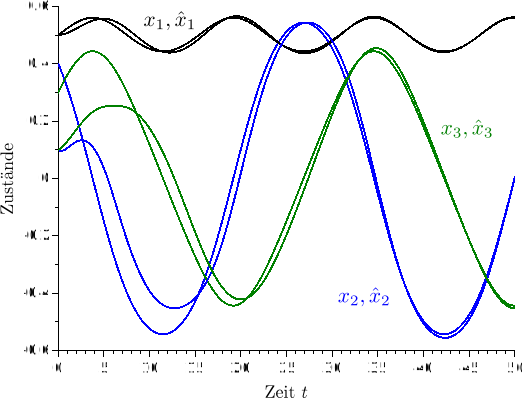
\includegraphics[width=0.8\textwidth]{Kreisel_HG}
\par\end{centering}
\caption{Simulation der Kreiselgleichungen und des zugehörigen High-Gain-Beobachters\label{fig:Kreisel-HG}}

\end{figure}

\begin{example}
\label{exa:wagen-pendel-hg1}Man betrachte das Wagen-Pendel-System
aus Abschnitt~\ref{subsec:Wagen-mit-Pendel}, allerdings ohne Eingang
($u=0$) und reibungsfrei ($d_{1}=0,$ $d_{2}=0$). Aus Gl.~(\ref{eq:modell-pendel-mit-wagen})
liest man das Vektorfeld 
\begin{equation}
f(x)=\left(\begin{array}{c}
x_{2}\\
\frac{m_{2}\sin x_{3}\left(g\cos x_{3}+\ell x_{4}^{2}\right)}{m_{1}+m_{2}\sin^{2}x_{3}}\\
x_{4}\\
-\frac{\sin x_{3}\left(g(m_{1}+m_{2})+\ell m_{2}x_{4}^{2}\cos x_{3}\right)}{\ell\left(m_{1}+m_{2}\sin^{2}x_{3}\right)}
\end{array}\right)\label{eq:hg-wagen-pendel-f0}
\end{equation}
ab. Als Ausgang verwenden wir zunächst die Position des Wagens, d.\,h.
$y_{1}=h_{1}(x)=x_{1}$ (siehe Abb.~\ref{fig:Wagen-mit-Pendel-Hig-Gain}).
Die Beobachtbarkeitsmatrix 
\begin{equation}
Q_{B}(x)=\left(\begin{array}{cccc}
1 & 0 & 0 & 0\\
0 & 1 & 0 & 0\\
0 & 0 & * & \frac{2\ell m_{2}x_{4}\sin x_{3}}{m_{1}+m_{2}\sin^{2}x_{3}}\\
0 & 0 & * & *
\end{array}\right)\label{eq:wageh-pendel-hg-Qb1}
\end{equation}
enthält in den letzten zwei Zeilen bzw. Spalten vergleichsweise komplizierte
Ausdrücke. Zur Überprüfung der Regularität der Beobachtbarkeitsmatrix
berechnen wir deren Determinante, für die man auch einen umfangreichen
Ausdruck erhält. Mit $\det Q_{B}(x)=(gm_{2}/m_{1})^{2}$ für $x_{3}=0$,
$x_{4}=0$ ist die Beobachtbarkeitsmatrix zumindest für kleine Auslenkungen
des Pendels und kleine Winkelgeschwindigkeiten regulär. Die Beobachterverstärkung
\[
k(\hat{x})=Q_{B}^{-1}(x)\cdot\left(\begin{array}{c}
a_{3}\\
a_{2}\\
a_{1}\\
a_{0}
\end{array}\right)=\left(\begin{array}{c}
a_{3}\\
a_{2}\\
*\\
*
\end{array}\right)
\]
nach Gl.~(\ref{eq:hg-beobachter-autonom-orig}) enthält in den letzten
zwei Komponenten ebenfalls sehr umfangreiche Ausdrücke, so dass auf
die vollständige Angabe verzichtet wird.
\end{example}
\begin{figure}
\begin{centering}
\resizebox{0.5\textwidth}{!}{\input{wagen_pendel_high_gain.pdftex_t}}
\par\end{centering}
\caption{Wagen mit Pendel\label{fig:Wagen-mit-Pendel-Hig-Gain}}
\end{figure}

\begin{example}
\label{exa:wagen-pendel-hg2}Wir betrachten erneut das Wagen-Pendel-System
aus Beispiel~\ref{exa:wagen-pendel-hg1}, verwenden jetzt aber die
horizontale Position der Last als Ausgang, d.\,h. $y_{2}=h_{2}(x)=x_{1}+\ell\sin x_{3}$
(vgl. Abb.~\ref{fig:Wagen-mit-Pendel-Hig-Gain}). Die zugehörige
Beobachtbarkeitsmatrix hat die Form 
\[
Q_{B}(x)=\left(\begin{array}{cccc}
1 & 0 & \ell\cos x_{3} & 0\\
0 & 1 & -\ell x_{4}\sin x_{3} & \ell\cos x_{3}\\
0 & 0 & * & -\frac{2\ell m_{1}x_{4}\sin x_{3}}{m_{1}+m_{2}\sin^{2}x_{3}}\\
0 & 0 & * & *
\end{array}\right).
\]
Mit $\det Q_{B}(x)=g^{2}$ für $x_{3}=0$, $x_{4}=0$ ist die Beobachtbarkeitsmatrix
auch mit diesem Ausgang für kleine Auslenkungen und kleine Winkelgeschwindigkeiten
regulär. Damit kann man den Beobachter~(\ref{eq:hg-beobachter-autonom-orig})
berechnen, erhält aber wiederum umfangreiche Ausdrücke.
\end{example}

Für die Konvergenzanalyse betrachten wir das System~(\ref{eq:hg-system-autonom})
und den Beobachter~(\ref{eq:hg-beobachter-autonom-trans}) in den
transformierten Koordinaten. Genügt die in der Fehlerdifferentialgleichung~(\ref{eq:hg-fehlerdyn})
auftretende Nichtlinearität~$\alpha$ einer Lipschitz-Bedingung\index{Lipschitz-Bedingung}
\begin{equation}
\forall\xi,\hat{\xi}:\quad\left\Vert \alpha(\xi)-\alpha(\hat{\xi})\right\Vert \leq\rho\left\Vert \xi-\hat{\xi}\right\Vert \label{eq:hg-lipschitz-bedingung}
\end{equation}
mit der Lipschitz-Konstanten $\rho>0$, dann kann über die Wahl der
Beobachterverstärkung~$l$ durch den linearen Teil $A-lc^{T}$ die
Konvergenz des Beobachters gesichert werden. Der folgende Satz trifft
eine globale Konvergenzaussage:
\begin{theorem}
\label{thm:hg-konvergenz-autonom}Gegeben sei System~(\ref{eq:hg-system-autonom})
zusammen mit dem Beobachter~(\ref{eq:hg-beobachter-autonom-orig}).
Das Vektorfeld~$f$ sei auf $\mathcal{M}=\R^{n}$ definiert und vollständig.
Die Beobachtbarkeitsabbildung~$q$ sei ein globaler Diffeomorphismus.
Außerdem genüge die Nichtlinearität~$\alpha$ der globalen Lipschitz-Bedingung~(\ref{eq:hg-lipschitz-bedingung}).
Dann existiert ein Vektor $l\in\R^{n}$ derart, dass 
\begin{equation}
\lim_{t\to\infty}\left\Vert \hat{x}(t)-x(t)\right\Vert =0\label{eq:hg-konvergenz}
\end{equation}
für alle Anfangswerte $x(0),\hat{x}(0)\in\mathcal{M}$ gilt.
\end{theorem}

Die Beweise in~\cite{gauthier92,ciccarella93,dalla-mora1997} basieren
auf sehr speziellen Eigenwertvorgaben. In späteren Arbeiten entfällt
diese Einschränkung. Der folgende Beweis beruht auf~\cite{roebenack2012ssd,roebenack2016sac}:\nocite{derbel2016sac}
\begin{svmultproof2}
Laut Annahme ist die Beobachtbarkeitsabbildung ein globaler Diffeomorphismus.
Wir führen daher die Konvergenzanalyse in den transformierten Koordinaten
durch und zeigen, dass die Ruhelage $\tilde{\xi}=0$ der Fehlerdifferentialgleichung~(\ref{eq:hg-fehlerdyn})
global asymptotisch stabil ist. Definiert man 
\begin{equation}
\Delta\alpha(\tilde{\xi},t):=\alpha(\xi)-\alpha(\hat{\xi}),\label{eq:hg-delta-alpha}
\end{equation}
dann lässt sich die Fehlerdifferentialgleichung~(\ref{eq:hg-fehlerdyn})
als Verknüpfung eines linearen zeitinvarianten Systems mit der Übertragungsfunktion
\[
G(s)=\left(sI-\left(A-lc^{T}\right)\right)^{-1}b=\frac{1}{\CP(s)}\left(\begin{array}{c}
1\\
s+a_{n-1}\\
s^{2}+a_{n-1}s+a_{n-2}\\
\vdots
\end{array}\right)
\]
und der zeitvarianten Nichtlinearität~(\ref{eq:hg-delta-alpha})
darstellen (vgl. Abb.~\ref{fig:Fehlerdynamik-High-Gain}). Wir gehen
davon aus, dass~(\ref{eq:hg-cp}) als Hurwitz-Polynom vorgegeben
wurde. Damit besitzt das lineare Teilsystem eine endliche Verstärkung,
d.\,h. $\|G\|_{\infty}<\infty$.
\begin{figure}
\begin{centering}
\resizebox{0.82\textwidth}{!}{\input{high-gain-nf1.pdftex_t}}
\par\end{centering}
\caption{Struktur der Fehlerdynamik~(\ref{eq:hg-fehlerdyn}) des High-Gain-Beobachters~(\ref{eq:hg-beobachter-autonom-trans})\label{fig:Fehlerdynamik-High-Gain}}
\end{figure}

Führt man bei der Beobachterverstärkung $l^{\epsilon}=(a_{n-1}/\epsilon,\ldots,a_{0}/\epsilon^{n})^{T}$
einen Skalierungsfaktor $\epsilon\in(0,1]$ ein, so erhält man das
in~$\epsilon$ parametrierte charakteristische Polynom
\begin{equation}
\begin{array}{lrl}
\CP^{\epsilon}(s) & := & \det(sI-A+l^{\epsilon}c^{T})\\
 & = & \frac{a_{0}}{\epsilon^{n}}+\frac{a_{1}}{\epsilon^{n-1}}s+\cdots+\frac{a_{n-1}}{\epsilon}s^{n-1}+s^{n}\\
 & = & \left(s-\frac{s_{1}}{\epsilon}\right)\cdots\left(s-\frac{s_{n}}{\epsilon}\right).
\end{array}\label{eq:hg-cp-epsilon}
\end{equation}
Für $\epsilon\to0$ entspricht diese Skalierung einer Streckung der
Eigenwerte nach links. Die zugehörige Übertragungsfunktion hat dann
die Form
\[
G^{\epsilon}(s)=\left(sI-\left(A-l^{\epsilon}c^{T}\right)\right)^{-1}b=\frac{1}{\CP^{\epsilon}(s)}\left(\begin{array}{c}
1\\
s+a_{n-1}\epsilon^{-1}\\
s^{2}+a_{n-1}\epsilon^{-1}s+a_{n-2}\epsilon^{-2}\\
\vdots
\end{array}\right).
\]
Für den Frequenzgang der $i$-ten Komponente gilt
\[
\begin{array}{ccl}
G_{i}^{\epsilon}(j\omega) & = & \frac{(j\omega)^{i-1}+\frac{a_{n-1}}{\epsilon}(j\omega)^{i-2}+\cdots+\frac{a_{n-i+1}}{\epsilon^{i-1}}}{\left(j\omega-\frac{s_{1}}{\epsilon}\right)\cdots\left(j\omega-\frac{s_{n}}{\epsilon}\right)}\\
 & = & \frac{(j\omega\epsilon)^{i-1}+a_{n-1}(j\omega\epsilon)^{i-2}+\cdots+a_{n-i+1}}{\left(j\omega\epsilon-s_{1}\right)\cdots\left(j\omega\epsilon-s_{n}\right)}\epsilon^{n-i+1}\\
 & = & \frac{(j\tilde{\omega})^{i-1}+a_{n-1}(j\tilde{\omega})^{i-2}+\cdots+a_{n-i+1}}{\left(j\tilde{\omega}-s_{1}\right)\cdots\left(j\tilde{\omega}-s_{n}\right)}\epsilon^{n-i+1}\\
 & = & G_{i}(j\tilde{\omega})\epsilon^{n-i+1}
\end{array}
\]
mit $\tilde{\omega}=\omega\epsilon$. Daraus folgt unmittelbar $\|G_{i}^{\epsilon}\|_{\infty}=\|G_{i}\|_{\infty}\epsilon^{n-i+1}\to0$
für $\epsilon\to0$. Somit lassen sich der Parameter~$\epsilon$
und damit die zugehörige Beobachterverstärkung~$l^{\epsilon}$ immer
so wählen, dass $\|G^{\epsilon}\|_{\infty}<1/\rho$. Mit einer derartigen
Wahl der Beobachterverstärkung im linearen Teilsystem ist die Gesamtverstärkung
des offenen Kreises kleiner als Eins. Nach dem Satz über die kleine
Kreisverstärkung ist die Ruhelage $\tilde{\xi}=0$ global asymptotisch
stabil, so dass die Konvergenz~(\ref{eq:hg-konvergenz}) gesichert
ist (siehe Anhang~\ref{sec:Stabilitaet-im-geschlossenen-Regelkreis}).
\end{svmultproof2}

\begin{remark}
Für die korrekte Festlegung der Beobachterverstärkung~$l$ ist die
Kenntnis der Lipschitz-Konstanten~$\rho$ aus Ungl.~(\ref{eq:hg-lipschitz-bedingung})
erforderlich. Die exakte Bestimmung der Lipschitz-Konstanten ist in
der Regel aufwendig. Alternativ könnte man versuchen, über Intervallarithmetik
eine Abschätzung der Lipschitz-Konstanten zu erhalten. Praktisch gibt
man zunächst Eigenwerte $s_{1},\ldots,s_{n}$ für ein stabiles charakteristisches
Polynom~(\ref{eq:hg-cp}) vor. Dann geht man zum charakteristischen
Polynom~(\ref{eq:hg-cp-epsilon}) mit $\epsilon=1$ über und verkleinert
$\epsilon>0$ solange, bis der Boebachter konvergiert. 
\end{remark}

\subsection{Beobachtbarkeit und Beobachterentwurf für eingangsabhängige Systeme\label{subsec:Beobachterentwurf-mit-eingang}}

Im Folgenden wird das in Abschnitt~\ref{subsec:Beobachtbarkeit-autonom}
zunächst für autonome Systeme eingeführte Konzept der Beobachtbarkeit
auf eingangsabhängige Systeme übertragen, um anschließend auch für
diese Systeme den Beobachter aus Abschnitt~\ref{subsec:Beobachterentwurf-autonom}
verwenden zu können.

Für die Beobachtbarkeitsanalyse betrachten wir das System~(\ref{eq:hg-system-nicht-affin})
auf dem Zeit\-inter\-vall $[0,T]$ mit $T>0$. Das Eingangssignal
$u(\cdot)$ sei auf diesem Zeit\-inter\-vall (mindestens) stückweise
stetig. Dann besitzt das System für hinreichend kleine $T>0$ ein
allgemeine Lösung, die wir in leichter Modifikation der bisherigen
Notation mit $\varphi_{t}^{u}$ bezeichnen (vgl. Abschnitt~\ref{sec:Vektorfelder-und-Fluesse}).
Zwei Zustände $p,\bar{p}\in\mathcal{M}$ heißen \emph{nicht unterscheidbar
bezüglich eines (gegebenen) Eingangssignals} $u(\cdot)$\index{Nichtunterscheidbarkeit!bezüglich eines Eingangssignals},
wenn die zugehörigen Verläufe der Ausgänge übereinstimmen, d.\,h.
\[
\forall t\in[0,T]:\quad h(\varphi_{t}^{u}(p))=h(\varphi_{t}^{u}(\bar{p})).
\]
Mit dem Begriff der Unterscheidbarkeit lassen sich in Analogie zu
Abschnitt~\ref{subsec:Beobachtbarkeit-autonom} auch lokale und globale
Beobachtbarkeit für eingangsabhängige Systeme definieren. Das folgende
Beispiel zeigt, dass bei einem nichtlinearen System die Möglichkeit,
den Zustand aus dem Verlauf des Ausgangs und seinen Zeitableitungen
zu rekonstruieren, vom konkreten Eingangssignal abhängen kann:

\begin{example}
\label{exa:Minisystem-nicht-glm-beob}Gegeben sei das System
\begin{equation}
\begin{array}{lcl}
\dot{x}_{1} & = & -x_{1}+x_{2}(1+u)\\
\dot{x}_{2} & = & x_{2}\\
y & = & x_{1}.
\end{array}\label{eq:Minisystem-nicht-glm-beob}
\end{equation}
Für $u\neq-1$ erhält man den Zustand~$x$ aus dem Ausgang~$y$
und seiner ersten Zeitableitung:
\[
\left.\begin{array}{lcl}
y & = & x_{1}\\
\dot{y} & = & -x_{1}+x_{2}(1+u)
\end{array}\right\} \quad\Longrightarrow\quad\begin{array}{lcl}
x_{1} & = & y,\\
x_{2} & = & \frac{y+\dot{y}}{1+u}.
\end{array}
\]
Für $u\equiv-1$ wirkt sich dagegen der Zustand~$x_{2}$ nicht auf
den Ausgang aus. In diesem Fall sind alle Anfangszustände, die in
der ersten Komponente übereinstimmen, nicht unterscheidbar.
\end{example}

Das Beispiel verdeutlicht, dass es sinnvoll sein kann, die Beobachtbarkeit
eines eingangsabhängigen Systems derart zu definieren, dass diese
Eigenschaft unabhängig vom gewählten Eingangssignal ist. Wir nennen
ein System~(\ref{eq:hg-system-eingangsaffin}) \emph{gleichmäßig
lokal} bzw. \emph{global beobachtbar}, wenn es für alle zulässigen
Eingangssignale $u(\cdot)$ lokal bzw. global beobachtbar ist. 

Gegeben sei ein eingangsaffines System
\begin{equation}
\dot{x}=f(x)+g(x)u,\quad y=h(x)\label{eq:hg-system-eingangsaffin}
\end{equation}
mit den Vektorfeldern $f,g:\mathcal{M}\to\R^{n}$ und dem Skalarfeld
$h:\mathcal{M}\to\R$. Die Felder seien hinreichend glatt. Erfüllt
der autonome Teil~(\ref{eq:hg-system-autonom}) von System~(\ref{eq:hg-system-eingangsaffin})
die Bedingungen von Lemma~\ref{lem:Beobachtbarkeit-hinreichende-Bedingung},
so ist eine Beurteilung der gleichmäßigen lokalen Beobachtbarkeit
anhand der Beobachtbarkeitsnormalform\index{Beobachtbarkeitsnormalform}\index{Normalform!Beobachtbarkeits-}
möglich~\cite{gauthier81,gauthier92}:
\begin{theorem}
\label{thm:hg-Beobachtbarkeit-nicht-autonom}Man betrachte das System~(\ref{eq:hg-system-eingangsaffin})
im Punkt $p\in\mathcal{M}$. Es gelte $\rank\,Q_{B}(p)=n$. Das System
ist genau dann gleichmäßig lokal beobachtbar im Punkt~$p$, wenn
es zustands\-äquivalent zur Form 
\begin{equation}
\begin{array}{lcl}
\dot{\xi}_{1} & = & \xi_{2}+\beta_{1}(\xi_{1})u\\
\dot{\xi}_{2} & = & \xi_{3}+\beta_{2}(\xi_{1},\xi_{2})u\\
 & \vdots\\
\dot{\xi}_{n-1} & = & \xi_{n}+\beta_{n-1}(\xi_{1},\xi_{2},\ldots,\xi_{n-1})u\\
\dot{\xi}_{n} & = & \alpha(\xi)+\beta_{n}(\xi_{1},\xi_{2},\ldots,\xi_{n-1},\xi_{n})u\\
y & = & \xi_{1}
\end{array}\label{eq:Beobachtbarkeits-NF-nicht-autonom}
\end{equation}
ist.
\end{theorem}
\begin{svmultproof2}
Es gelte $\rank\,Q_{B}(p)=n$. Dann ist die in Gl.~(\ref{eq:Beobachtbarkeitsabbildung})
definierte Beobachtbarkeitsabbildung $\xi=q(x)$ ein lokaler Diffeomorphismus,
der das System~(\ref{eq:hg-system-eingangsaffin}) in die Beobachtbarkeitsnormalform\index{Beobachtbarkeitsnormalform}\index{Normalform!Beobachtbarkeits-}
\begin{equation}
\begin{array}{lcl}
\dot{\xi}_{1} & = & \xi_{2}+\beta_{1}(\xi)u\\
\dot{\xi}_{2} & = & \xi_{3}+\beta_{2}(\xi)u\\
 & \vdots\\
\dot{\xi}_{n-1} & = & \xi_{n}+\beta_{n-1}(\xi)u\\
\dot{\xi}_{n} & = & \alpha(\xi)+\beta_{n}(\xi)u\\
y & = & \xi_{1}
\end{array}\label{eq:Beobachtbarkeits-NF-nicht-autonom-allgemein}
\end{equation}
mit $\alpha(\xi):=L_{f}^{n}h(q^{-1}(\xi))$ und 
\begin{equation}
\beta_{i}(\xi):=L_{g}L_{f}^{i-1}h(q^{-1}(\xi))\quad\text{für}\quad i=1,\ldots,n\label{eq:beobachtbarkeits-NF-beta-i}
\end{equation}
überführt (vgl. Beweis von Satz~\ref{thm:hg-beobachtbarkeitsnormalform}).
Für die nachfolgenden Untersuchungen betrachten wir zwei Instanzen
des Systems~(\ref{eq:Beobachtbarkeits-NF-nicht-autonom-allgemein}),
nämlich eine mit dem Zustand~$\xi$ und dem Anfangswert $\xi(0)$
und eine weitere Instanz mit dem Zustand~$\bar{\xi}$ und dem Anfangswert
$\bar{\xi}(0)$. Beide Instanzen werden mit dem gleichen Eingangssignal~$u$
beaufschlagt.

\notwendig\ Wir zeigen die Notwendigkeit der Form~(\ref{eq:Beobachtbarkeits-NF-nicht-autonom})
indirekt. Wir nehmen also an, dass das System~(\ref{eq:Beobachtbarkeits-NF-nicht-autonom-allgemein})
nicht der speziellen Struktur~(\ref{eq:Beobachtbarkeits-NF-nicht-autonom})
genügt. Sei $i_{0}<n$ die kleinste Zahl, so dass eine Zahl $j_{0}>i_{0}$
mit $\partial\beta_{i_{0}}/\partial\xi_{j_{0}}\not\equiv0$ existiert.
(Das bedeutet, dass $\beta_{i_{0}}(\xi)$ nicht nur von $\xi_{1},\ldots,\xi_{i_{0}}$,
sondern auch von $\xi_{j_{0}}$ abhängt.) Die Anfangswerte $\xi(0)\neq\bar{\xi}(0)$
beider Systeminstanzen seien so gewählt, dass sie in den ersten~$i_{0}$
Komponenten übereinstimmen, d.\,h. $\xi_{i}(0)=\bar{\xi}_{i}(0)$
für $i=1,\ldots,i_{0}$. Wegen $\partial\beta_{i_{0}}/\partial\xi_{j_{0}}\not\equiv0$
lassen sich zusätzlich die $j_{0}$-ten Komponenten $\xi_{j_{0}}(0)\neq\bar{\xi}_{j_{o}}(0)$
beider Anfangswerte so wählen, dass $\beta_{i_{0}}(\xi(0))-\beta_{i_{0}}(\bar{\xi}(0))\neq0$
gilt. Die Rückführung 
\begin{equation}
u=-\frac{\xi_{i_{0}+1}-\bar{\xi}_{i_{0}+1}}{\beta_{i_{0}}(\xi)-\beta_{i_{0}}(\bar{\xi})}\label{eq:beweis-struktur-nicht-autonom-u}
\end{equation}
ist damit zumindest für ein gewisses Zeitintervall $[0,T]$ bei hinreichend
kleiner Endzeit $T>0$ definiert. Die Abweichung in der $i_{0}$-ten
Differentialgleichung beider Instanzen verschwindet unter Wirkung
des Eingangssignals~(\ref{eq:beweis-struktur-nicht-autonom-u}) identisch:
\[
\dot{\xi}_{i_{0}}-\dot{\bar{\xi}}_{i_{0}}=\xi_{i_{0}+1}+\bar{\xi}_{i_{0}+1}+\left(\beta_{i_{0}}(\xi)-\beta_{i_{0}}(\bar{\xi})\right)u\equiv0.
\]
Dann stimmen die Zeitverläufe in den ersten $i_{0}$ Komponenten von
$\xi,\bar{\xi}$ auf dem Intervall $[0,T]$ überein und führen somit
unabhängig von den Anfangswerten der letzten $n-i_{0}$ Komponenten
zu dem gleichen Ausgangsverlauf. Damit sind alle Anfangswerte $\xi(0),\bar{\xi}(0)$,
die in den ersten $i_{0}$ Komponenten übereinstimmen, für den Eingangsverlauf~(\ref{eq:beweis-struktur-nicht-autonom-u})
nicht unterscheidbar. Das System ist also nicht gleichmäßig lokal
beobachtbar.

\hinreichend\ Das transformierte System~(\ref{eq:Beobachtbarkeits-NF-nicht-autonom-allgemein})
besitze die Struktur~(\ref{eq:Beobachtbarkeits-NF-nicht-autonom}).
Für beide Instanzen des Systems~(\ref{eq:Beobachtbarkeits-NF-nicht-autonom})
betrachten wir beliebige Verläufe von dem Ausgang $y(t)=\xi_{1}(t)=\bar{\xi}_{1}(t)$
und dem Eingang $u(t)$ für alle $t\in[0,T]$ mit $T>0$. Durch Einsetzen
in die erste Differentialgleichung von~(\ref{eq:Beobachtbarkeits-NF-nicht-autonom})
erhält man übereinstimmende Verläufe $\xi_{2}(t)=\bar{\xi}_{2}(t)$,
aus der zweiten Differentialgleichung folgt $\xi_{3}(t)=\bar{\xi}_{3}(t)$.
Dieses Verfahren setzt man bis zur vorletzen Differentialgleichung
fort, aus der man $\xi_{n}(t)=\bar{\xi}_{n}(t)$ für alle $t\in[0,T]$
erhält. Damit gilt $\xi(t)=\bar{\xi}(t)$ für alle $t\in[0,T]$, so
dass auch die Anfangswerte beider Systeminstanzen übereinstimmen:
$\xi(0)=\bar{\xi}(0)$. Für einen vorgegebenen Ausgangsverlauf ist
unabhängig vom konkreten Eingangsverlauf der Anfangswert eindeutig
festgelegt. Das System~(\ref{eq:Beobachtbarkeits-NF-nicht-autonom})
ist daher gleichmäßig beobachtbar.
\end{svmultproof2}

Die Argumentation im hinreichenden Teil des Beweises lässt unmittelbar
eine Verallgemeinerung auf nicht eingangsaffine Systeme mit ggf. vektorwertigem
Eingang zu:
\begin{corollary}
\label{cor:Beobachtbarkeit-nicht-affin-MISO}Gegeben sei ein System
\[
\dot{x}=f(x)+\tilde{g}(x,u),\quad y=h(x)
\]
mit hinreichend glatten Feldern $f:\mathcal{M}\to\R^{n}$, $\tilde{g}:\mathcal{M}\times\mathcal{U}\to\R^{n}$,
$h:\mathcal{M}\to\R$ und $\mathcal{U}\subseteq\R^{m}$. Für das zugeordnete
autonome System~(\ref{eq:hg-system-autonom}) gelte $\rank\,Q_{B}(p)=n$
in einem Punkt $p\in\mathcal{M}$. Ist das System in einer Umgebung
von~$p$ zustands\-äquivalent zur Form
\begin{equation}
\begin{array}{lcl}
\dot{\xi}_{1} & = & \xi_{2}+\tilde{\beta}_{1}(\xi_{1},u)\\
\dot{\xi}_{2} & = & \xi_{3}+\tilde{\beta}_{2}(\xi_{1},\xi_{2},u)\\
 & \vdots\\
\dot{\xi}_{n-1} & = & \xi_{n}+\tilde{\beta}_{n-1}(\xi_{1},\xi_{2},\ldots,\xi_{n-1},u)\\
\dot{\xi}_{n} & = & \alpha(\xi)+\tilde{\beta}_{n}(\xi_{1},\xi_{2},\ldots,\xi_{n-1},\xi_{n},u)\\
y & = & \xi_{1},
\end{array}\label{eq:Beobachtbarkeits-NF-nicht-affin}
\end{equation}
dann ist es im Punkt~$p$ gleichmäßig lokal beobachtbar.
\end{corollary}

Für einige eingangsaffine Beispielssysteme wird die Existenz der speziellen
Form~(\ref{eq:Beobachtbarkeits-NF-nicht-autonom}) untersucht:

\begin{example}
\label{exa:Minisystem-nicht-glm-Beobachtbarkeits-NF}Das System~(\ref{eq:Minisystem-nicht-glm-beob})
aus Beispiel~\ref{exa:Minisystem-nicht-glm-beob} besitzt eine lineare
Beobachtbarkeitsabbildung~(\ref{eq:Beobachtbarkeitsabbildung}) und
folglich eine konstante Beobachtbarkeitsmatrix~(\ref{eq:Beobachtbarkeitsmatrix}):
\[
\xi=q(x)=\left(\begin{array}{c}
x_{1}\\
-x_{1}+x_{2}
\end{array}\right),\quad Q_{B}(x)=q^{\prime}(x)=\left(\begin{array}{rc}
1 & 0\\
-1 & 1
\end{array}\right).
\]
Damit ist die Umkehrtransformation $x=q^{-1}(\xi)$ auch linear: $x_{1}=\xi_{1}$,
$x_{2}=\xi_{1}+\xi_{2}$. Das transformierte System lautet
\[
\begin{array}{lcl}
\dot{\xi} & = & \frac{\d}{\d t}q(x)\\
 & = & q^{\prime}(x)\cdot\dot{x}\\
 & = & Q_{B}(x)\left(f(x)+g(x)u\right)\\
 & = & \left.\left(\begin{array}{rc}
1 & 0\\
-1 & 1
\end{array}\right)\left(\begin{array}{c}
-x_{1}+x_{2}(1+u)\\
x_{2}
\end{array}\right)\right|_{x=q^{-1}(\xi)}\\
 & = & \left(\begin{array}{c}
\xi_{2}+(\xi_{1}+\xi_{2})u\\
\xi_{1}-(\xi_{1}+\xi_{2})u
\end{array}\right).
\end{array}
\]
Das System liegt damit in der Form~(\ref{eq:Beobachtbarkeits-NF-nicht-autonom-allgemein})
mit $\beta_{1}(\xi)=\xi_{1}+\xi_{2}$ und $\beta_{2}(\xi)=-(\xi_{1}+\xi_{2})$
vor. Da $\beta_{1}(\xi)$ auch von~$\xi_{2}$ abhängt, ist die Struktur~(\ref{eq:Beobachtbarkeits-NF-nicht-autonom})
nicht gegeben. Das System ist also in Übereinstimmung mit den Betrachtungen
aus Beispiel~\ref{exa:Minisystem-nicht-glm-beob} nicht gleichmäßig
lokal beobachtbar.
\end{example}

\begin{example}
\label{exa:hg-mathematisches-Pendel-Drehmoment}Das inverse mathematische
Pendel aus Beispiel~\ref{exa:hg-inverses-pendel} mit der Ausgangsgröße
aus Beispiel~\ref{exa:hg-mathematisches-Pendel-autonom} lässt sich
durch das Zustandsraummodell
\begin{equation}
\begin{array}{lcl}
\dot{x}_{1} & = & x_{2}\\
\dot{x}_{2} & = & \kappa_{1}\sin x_{1}+\kappa_{2}u\\
y & = & x_{2}
\end{array}\label{eq:hg-math-pendel-drehmoment}
\end{equation}
beschreiben. Aus der Beobachtbarkeitsabbildung~(\ref{eq:hg-math-pendel-q})
erhält man Hin- und Rücktransformation 
\[
\begin{array}{lcl}
\xi_{1} & = & x_{2}\\
\xi_{2} & = & \kappa_{1}\sin x_{1}
\end{array}\qquad\text{und}\qquad\begin{array}{lcl}
x_{1} & = & \arcsin\frac{\xi_{2}}{\kappa_{1}}\\
x_{2} & = & \xi_{1}
\end{array}
\]
in die Beobachtbarkeitsnormalform~(\ref{eq:Beobachtbarkeits-NF-nicht-autonom-allgemein}).
Daraus ergibt sich das transformierte System 
\begin{equation}
\begin{array}{lcl}
\dot{\xi}_{1} & = & \xi_{2}+\kappa_{2}u\\
\dot{\xi}_{2} & = & \kappa_{1}\xi_{1}\sqrt{1-\frac{\xi_{2}^{2}}{\kappa_{1}^{2}}}
\end{array}\label{eq:hg-math-pendel-transformiert}
\end{equation}
mit $\beta_{1}(\xi)=\kappa_{2}$ und $\beta_{2}(\xi)=0$. Dabei hängt
$\beta_{1}(\xi)$ nicht von~$\xi_{2}$ ab, so dass das System~(\ref{eq:hg-math-pendel-transformiert})
in de Form~(\ref{eq:Beobachtbarkeits-NF-nicht-autonom}) vorliegt
und für $|x_{1}|<\pi/2$ nach Satz~\ref{thm:hg-Beobachtbarkeit-nicht-autonom}
gleichmäßig lokal beobachtbar ist. Mit der Beobachterverstärkung~(\ref{eq:math-pendel-autonom-beobachterverstaerkung-x})
erhält man für das erregte System~(\ref{eq:hg-math-pendel-drehmoment})
den Beobachter
\[
\left(\begin{array}{l}
\dot{\hat{x}}_{1}\\
\dot{\hat{x}}_{2}
\end{array}\right)=\left(\begin{array}{c}
\hat{x}_{2}\\
\kappa_{1}\sin\hat{x}_{1}+\kappa_{2}u
\end{array}\right)+\left(\begin{array}{c}
\frac{a_{0}}{\kappa_{1}\cos\hat{x}_{1}}\\
a_{1}
\end{array}\right)\left(y-\hat{x}_{2}\right)
\]
mit den Koeffizienten $a_{0},a_{1}>0$.
\end{example}

\begin{example}
\label{exa:Synchronmaschine-HG}In~\cite{mukhopadhyay1972} wird
eine Synchronmaschine\index{Synchronmaschine} modelliert und durch
die Zustandsgleichungen 
\begin{equation}
\begin{array}{lcl}
\dot{x}_{1} & = & x_{2}\\
\dot{x}_{2} & = & B_{1}-A_{1}x_{2}-A_{2}x_{3}\sin x_{1}-\tfrac{1}{2}B_{2}\sin(2x_{1})\\
\dot{x}_{3} & = & u-D_{1}x_{3}+D_{2}\cos x_{1}\\
y & = & x_{1}
\end{array}\label{eq:synchronmotor}
\end{equation}
beschrieben. Dabei bezeichnet~$x_{1}$ den Polradwinkel, also den
Winkel zwischen dem Polrad und dem Drehfeld. Der Polradwinkel fungiert
zugleich als Ausgangsgröße, welche aus dem mit einen Winkelencoder
erfassten Drehwinkel berechnet wird. Fernen seien $x_{2}$ die zugehörige
Winkelgeschwindigkeit (relativ zum rotierenden Bezugssystem), $x_{3}$
die Flussverkettung der Erregerwicklung und $u$ der Eingang.

Das Modell~(\ref{eq:synchronmotor}) wird häufig zu Vergleichszwecken
beim nichtlinearen Beobachterentwurf verwendet~\cite{keller86diss,birk88,adjallah94,roebenack2003buch,roebenack2005habil,adamy2014,franke2016pamm}.
Die Beobachtbarkeitsmatrix 
\begin{equation}
Q_{B}(x)=\left(\begin{array}{ccc}
1 & 0 & 0\\
0 & 1 & 0\\
-A_{2}x_{2}\cos x_{1}-B_{2}\cos(2x_{1}) & -A_{1} & -A_{2}\sin x_{1}
\end{array}\right)\label{eq:synchronmotor-beobachtbarkeitsmatrix}
\end{equation}
ist für $x_{1}\neq\pi i$ mit $i\in\mathbb{Z}$ regulär, so dass der
zugehörige autonome Systemteil, den man für $u=0$ erhält, in diesem
Bereich lokal beobachtbar ist. Zur Untersuchung der gleichmäßigen
Beobachtbarkeit betrachten wir die Struktur des aus~(\ref{eq:synchronmotor})
resultierenden Eingangsvektorfeldes $g(x)=\tfrac{\partial}{\partial x_{3}}$
in den transformierten Koordinaten:
\[
Q_{B}(x)\cdot g(x)=\left(\begin{array}{c}
0\\
0\\
-A_{2}\sin x_{1}
\end{array}\right).
\]
Mit $\beta_{1}(\cdot)=0$ und $\beta_{2}(\cdot)=0$ ist die Strukturbedingung~(\ref{eq:Beobachtbarkeits-NF-nicht-autonom})
erfüllt, so dass das System~(\ref{eq:synchronmotor}) im o.\,g.
Bereich gleichmäßig lokal beobachtbar ist. Die Beobachterverstärkung
hat die Form
\[
k(\hat{x})=Q_{B}^{-1}(\hat{x})\left(\begin{array}{c}
a_{2}\\
a_{1}\\
a_{0}
\end{array}\right)=\left(\begin{array}{c}
a_{2}\\
a_{1}\\
-\frac{a_{0}+a_{1}A_{1}+a_{2}A_{2}\hat{x}_{3}\cos\hat{x}_{1}+a_{2}B_{2}\cos(2\hat{x}_{1})}{A_{2}\sin\hat{x}_{1}}
\end{array}\right)
\]
mit den Koeffizienten $a_{0},a_{1},a_{2}>0$. Simulationsuntersuchungen
des Beobachters sind in~\cite{roebenack2003buch} beschrieben.
\end{example}

Bei komplizierteren Systemen lässt sich die Beobachtbarkeitsnormalform~(\ref{eq:Beobachtbarkeits-NF-nicht-autonom-allgemein})
in der Regel nicht explizit angeben. In diesen Fällen ist Satz~\ref{thm:hg-Beobachtbarkeit-nicht-autonom}
zur Überprüfung der gleichmäßigen Beobachtbarkeit nicht geeignet.
Mit folgendem Satz ist die Überprüfung der Struktur~(\ref{eq:Beobachtbarkeits-NF-nicht-autonom})
auch in Originalkoordinaten möglich~\cite[Lemma~2]{jo2002}:
\begin{theorem}
\label{thm:hg-Beobachtbarkeit-nicht-autonom2}Man betrachte das System~(\ref{eq:hg-system-eingangsaffin})
im Punkt $p\in\mathcal{M}$. Es gelte $\rank\,Q_{B}(p)=n$. Das System
ist genau dann gleichmäßig lokal beobachtbar im Punkt~$p$, wenn
\begin{equation}
\d L_{g}L_{f}^{i}h\in\spann\{\d h,\d L_{f}h,\ldots,\d L_{f}^{i}h\}\quad\text{für}\quad i=0,\ldots,n-2\label{eq:beob-nicht-autonom-grad-x}
\end{equation}
in einer Umgebung von~$p$ gilt.
\end{theorem}
\begin{svmultproof2}
Es gelte $\rank\,Q_{B}(p)=n$. Dann ist die in Gl.~(\ref{eq:Beobachtbarkeitsabbildung})
definierte Beobachtbarkeitsabbildung $\xi=q(x)$ ein lokaler Diffeomorphismus,
der das System~(\ref{eq:hg-system-eingangsaffin}) in die Beobachtbarkeitsnormalform~(\ref{eq:Beobachtbarkeits-NF-nicht-autonom-allgemein})
überführt. Die in Gl.~(\ref{eq:Beobachtbarkeits-NF-nicht-autonom})
angegebenen funkionalen Abhängigkeiten in den Komponenten~$\beta_{i}$
des (transformierten) Eingangsvektorfeldes lassen sich über lineare
Abhängigkeiten ausdrücken:
\begin{equation}
\begin{array}{lclcl}
\beta_{1}(\xi_{1}) & \quad\Longleftrightarrow\quad & \d\beta_{1} & \in & \spann\{\d\xi_{1}\}\\
\beta_{2}(\xi_{1},\xi_{2}) & \quad\Longleftrightarrow\quad & \d\beta_{2} & \in & \spann\{\d\xi_{1},\d\xi_{2}\}\\
 & \vdots\\
\beta_{n-1}(\xi_{1},\xi_{2},\ldots,\xi_{n-1}) & \quad\Longleftrightarrow\quad & \d\beta_{n-1} & \in & \spann\{\d\xi_{1},\d\xi_{2},\ldots,\d\xi_{n-1}\}.
\end{array}\label{eq:beob-nicht-autonom-grad-z}
\end{equation}
Aus $\xi_{i}=L_{f}^{i-1}h(x)$ ergibt sich $\d\xi_{i}=\d L_{f}^{i-1}h(x)$
für $i=1,\ldots,n$. Mit~(\ref{eq:beobachtbarkeits-NF-beta-i}) wertet
Gl.~(\ref{eq:beob-nicht-autonom-grad-x}) die in Gl.~(\ref{eq:beob-nicht-autonom-grad-z})
beschriebenen Abhängigkeiten in den Originalkoordinaten aus. Die Anwendung
von Satz~\ref{thm:hg-Beobachtbarkeit-nicht-autonom} liefert den
Bezug zur gleichmäßigen lokalen Beobachtbarkeit.
\end{svmultproof2}

\begin{example}
Wir ergänzen das in Beispiel~\ref{exa:wagen-pendel-hg1} betrachtete
Wagen-Pendel-System um das Eingangsvektorfeld
\[
g(x)=\left(\begin{array}{c}
0\\
\frac{1}{m_{1}+m_{2}\sin^{2}x_{3}}\\
0\\
-\frac{\cos x_{3}}{l(m_{1}+m_{2}\sin^{2}x_{3})}
\end{array}\right)
\]
aus Abschnitt~\ref{subsec:Wagen-mit-Pendel}. Mit dem Vektorfeld~$f$
aus Gl.~(\ref{eq:hg-wagen-pendel-f0}) und dem Ausgang $y=h(x)=x_{1}$
berechnet man die Lie-Ableitungen 
\[
\begin{array}{lcl}
L_{g}h(x) & = & 0\\
L_{g}L_{f}h(x) & = & \frac{1}{m_{1}+m_{2}\sin^{2}x_{3}}\\
L_{g}L_{f}^{2}h(x) & = & -2\frac{m_{2}x_{4}\sin x_{3}\cos x_{3}}{(m_{1}+m_{2}\sin^{2}x_{3})^{2}},
\end{array}
\]
deren Gradienten die folgende Struktur aufweisen:
\[
\begin{array}{lcc}
\d L_{g}h & = & (\,0\,,\,0\,,\,0\,,\,0\,)\phantom{.}\\
\d L_{g}L_{f}h & = & (\,0\,,\,0\,,\,*\,,\,0\,)\phantom{.}\\
\d L_{g}L_{f}^{2}h & = & (\,0\,,\,0\,,\,*\,,\,*\,).
\end{array}
\]
Aus den ersten zwei Zeilen der Beobachtbarkeitsmatrix~(\ref{eq:wageh-pendel-hg-Qb1})
liest man $\d\xi_{1}=\d h=\d x_{1}$ und $\d\xi_{2}=\d L_{f}h=\d x_{2}$
ab. Damit ist Bedingung~(\ref{eq:beob-nicht-autonom-grad-x}) für
$i=1$ nicht erfüllt, d.\,h. aus $\d L_{g}L_{f}h\in\spann\{\d x_{3}\}$
folgt $\d L_{g}L_{f}h\notin\spann\{\d h,\d L_{f}h\}=\spann\{\d x_{1},\d x_{2}\}$.
Das System ist also nicht gleichmäßig beobachtbar.
\end{example}

\begin{remark}
Der beschriebene Zugang zum Entwurf von High-Gain-Beobachtern lässt
sich für Mehrgrößensysteme verallgemeinern~\cite{dalla-mora2000}.
Gleichzeitig zur Schätzung des Zustands ist grundsätzlich auch eine
Parameterschätzung mittels Adaption möglich~\cite{bullinger1997cdc,besancon2004}.
Erhält man für die Beobachtbarkeitsmatrix umfangreiche Ausdrücke,
so bietet sich die Berechnung mit algorithmischem Differenzieren an~\cite{rr2000nolta,roebenack2005dsmc,roebenack2005habil}.
Ist die Beobachtbarkeitsrangbedingung~(\ref{eq:Beobachtbarkeitsrangbedingung})
erfüllt, aber die Beobachtbarkeitsmatrix~(\ref{eq:Beobachtbarkeitsmatrix})
singulär, dann empfiehlt sich der Entwurf eines Einbettungsbeobachters~\cite{gauthier91}.\index{Beobachter!Einbettungs-}
\end{remark}

\section{Beobachterentwurf auf Basis der Eingangs-Ausgangs-Normalform\label{sec:High-Gain-Entwurf-Eingangs-Ausgangs-Normalform}}

\subsection{Struktur des Beobachters}

Die gleichmäßig lokale Beobachtbarkeit eines eingangsaffinen Systems~(\ref{eq:hg-system-eingangsaffin})
setzt die Zustandsäquivalenz zur Form~(\ref{eq:Beobachtbarkeits-NF-nicht-autonom})
voraus. Dabei unterliegen mit Ausnahme der letzten Komponente alle
anderen Komponenten des transformierten Eingangsvektorfeldes hinsichtlich
der zulässigen Abhängigkeiten bestimmten Strukturbedingungen. Bei
einem System mit wohldefiniertem relativen Grad würde der Eingang
nur in der letzten Differentialgleichungen des ersten Teilsystems
der Eingangs-Ausgangs-Normalform in Erscheinung treten. Die vorangegangenen
Komponenten des transformierten Eingangsvektorfeldes sind dabei identisch
Null, so dass das erste Teilsystem (unter Beachtung der zusätzlichen
Abhängigkeiten vom zweiten Teilsystem) der Strukturbedingung~(\ref{eq:Beobachtbarkeits-NF-nicht-autonom})
genügt. Dieser Abschnitt behandelt die in~\cite{jo2000b,roebenack2004at,roebenack2007ndst}
vorgestellten Entwurfsverfahren, bei denen der in Abschnitt~\ref{sec:High-Gain-Entwurf-Beobachtbarkeitsnormalform}
beschriebene Beobachterentwurf von der Beobachtbarkeitsnormalform
auf die Eingangs-Ausgang- bzw. Byrnes-Isidori-Normalform übertragen
wird.

Das eingangsaffine System~(\ref{eq:hg-system-eingangsaffin}) habe
einen wohldefinierten relativen Grad $r<n$. Dann kann das System
mit einer Zustandstransformation 
\begin{equation}
\left(\begin{array}{c}
\xi\\
\eta
\end{array}\right)=\Phi(x)\label{eq:hg-EA-Phi}
\end{equation}
 in die Eingangs-Ausgangs-Normalform
\begin{equation}
\left.\begin{array}{lcl}
\dot{\xi}_{1} & = & \xi_{2}\\
 & \vdots\\
\dot{\xi}_{r-1} & = & \xi_{r}\\
\dot{\xi}_{r} & = & \alpha(\xi,\eta)+\beta(\xi,\eta)u\\
\dot{\eta}_{1} & = & q_{1}(\xi,\eta)+d_{1}(\xi,\eta)u\\
 & \vdots\\
\dot{\eta}_{n-r} & = & q_{n-r}(\xi,\eta)+d_{n-r}(\xi,\eta)u\\
y & = & \xi_{1}
\end{array}\right\} \quad\begin{array}{rcl}
\dot{\xi} & = & A\xi+b(\alpha(\xi,\eta)+\beta(\xi,\eta)u)\\
\dot{\eta} & = & q(\xi,\eta)+d(\xi,\eta)u\\
y & = & c^{T}\xi
\end{array}\label{eq:hg-EA-NF}
\end{equation}
transformiert werden (siehe Abschnitt~\ref{subsec:Byrnes-Isidori-Normalform}).
Das erste Teilsystem besitzt weitgehend die Struktur der Beobachtbarkeitsnormalform~(\ref{eq:Beobachtbarkeits-NF-autonom}),
d.\,h., dass die Nichtlinearitäten, die hier zusätzlich über den
Eingang beeinflusst werden, nur in der letzten Zeile auftreten. Daher
wird der Beobachter für das erste Teilsystem auch in der Form analog
zu Gl.~(\ref{eq:hg-beobachter-autonom-trans}) angesetzt. Der Korrekturterm
wirkt nicht direkt auf das zweite Teilsystem. Insgesamt erhält man
dabei den Ansatz 
\begin{equation}
\begin{array}{rcl}
\dot{\hat{\xi}} & = & A\hat{\xi}+b(\alpha(\hat{\xi},\hat{\eta})+\beta(\hat{\xi},\hat{\eta})u)+l\cdot(y-\hat{\xi}_{1})\\
\dot{\hat{\eta}} & = & q(\hat{\xi},\hat{\eta})+d(\hat{\xi},\hat{\eta})u
\end{array}\label{eq:hg-EA-NF-Beobachter}
\end{equation}
mit der konstanten Beobachterverstärkung $l\in\R^{r}$. Der Beobachtungsfehler
$\tilde{\xi}=\xi-\hat{\xi}$ und $\tilde{\eta}=\eta-\hat{\eta}$ genügt
dem Differentialgleichungssystem
\begin{equation}
\begin{array}{lcl}
\dot{\tilde{\xi}} & = & \left(A-lc^{T}\right)\tilde{\xi}+b\left[\alpha(\xi,\eta)+\beta(\xi,\eta)u-\alpha(\hat{\xi},\hat{\eta})-\beta(\hat{\xi},\hat{\eta})u\right]\\
\dot{\tilde{\eta}} & = & q(\xi,\eta)+d(\xi,\eta)u-q(\hat{\xi},\hat{\eta})-d(\hat{\xi},\hat{\eta})u.
\end{array}\label{eq:hg-EA-fehler-dgl}
\end{equation}
In Anlehnung an Gl.~(\ref{eq:hg-cp}) erhält man mit $l=(a_{r-1},\ldots,a_{0})^{T}$
das charakteristische Polynom 
\begin{equation}
\begin{array}{crl}
\CP(s) & := & \det(sI-(A-lc^{T}))\\
 & = & a_{0}+a_{1}s+\cdots+a_{r-1}s^{r-1}+s^{r}\\
 & = & (s-s_{1})\cdots(s-s_{r}).
\end{array}\label{eq:hg-cp-EA-NF}
\end{equation}
Man würde Eigenwerte $s_{1},\ldots,s_{r}$, die hinreichend weit links
in der komplexen Ebene liegen, vorgeben und daraus die Koeffizienten
$p_{0},\ldots,p_{r-1}$ des charakteristischen Polynoms~(\ref{eq:hg-cp-EA-NF})
berechnen. Mit 
\[
\left(\begin{array}{c}
\dot{\hat{\xi}}\\
\dot{\hat{\eta}}
\end{array}\right)=\frac{\d}{\d t}\Phi(\hat{x})=\Phi^{\prime}(\hat{x})\cdot\dot{\hat{x}}
\]
lässt sich der Beobachter~(\ref{eq:hg-EA-NF-Beobachter}) in den
Originalkoordinaten angeben:
\begin{equation}
\begin{array}{lll}
\dot{\hat{x}} & = & \left(\Phi^{\prime}(\hat{x})\right)^{-1}\cdot\left(\begin{array}{c}
\dot{\hat{\xi}}\\
\dot{\hat{\eta}}
\end{array}\right)\\
 & = & \left(\Phi^{\prime}(\hat{x})\right)^{-1}\cdot\left(\begin{array}{c}
A\hat{\xi}+b(\alpha(\hat{\xi},\hat{\eta})+\beta(\hat{\xi},\hat{\eta})u)+l\cdot(y-\hat{\xi}_{1})\\
q(\hat{\xi},\hat{\eta})+d(\hat{\xi},\hat{\eta})u
\end{array}\right)\\
 & = & f(\hat{x})+g(\hat{x})u+\left(\Phi^{\prime}(\hat{x})\right)^{-1}\cdot\left(\begin{array}{c}
l\\
0
\end{array}\right)\cdot(y-h(\hat{x}))\\
 & =: & f(\hat{x})+g(\hat{x})u+k(\hat{x})\cdot(y-h(\hat{x})).
\end{array}\label{eq:hg-EA-Beobachter-x}
\end{equation}
Damit erhält man eine vom Beobachterzustand abhängige Beobachterverstärkung
$k:\mathcal{M}\to\R^{n}$. Anwendungen dieses Beobachteransatzes sind
beispielsweise in~\cite{gao2010,mahmud2011,ide2013,koester2015}
zu finden.

\subsection{Berechnung der Beobachterverstärkung auf Basis der Byrnes-Isidori-Normalform}

Eine besondere Situation liegt vor, wenn die Koordinatentransformation~(\ref{eq:hg-EA-Phi})
in die Eingangs-Ausgangs-Normalform~(\ref{eq:hg-EA-NF}) so gewählt
wird, dass $d\equiv0$ gilt. In diesem Fall geht~(\ref{eq:hg-EA-NF})
in die Byrnes-Isidori-Normalform 
\begin{equation}
\begin{array}{rcl}
\dot{\xi} & = & A\xi+b(\alpha(\xi,\eta)+\beta(\xi,\eta)u)\\
\dot{\eta} & = & q(\xi,\eta)\\
y & = & c^{T}\xi
\end{array}\label{eq:hg-BI-NF}
\end{equation}
über. Dabei vereinfacht sich die Fehlerdynamik~(\ref{eq:hg-EA-fehler-dgl})
zu 
\begin{equation}
\begin{array}{lcl}
\dot{\tilde{\xi}} & = & \left(A-lc^{T}\right)\tilde{\xi}+b\left[\alpha(\xi,\eta)+\beta(\xi,\eta)u-\alpha(\hat{\xi},\hat{\eta})-\beta(\hat{\xi},\hat{\eta})u\right]\\
\dot{\tilde{\eta}} & = & q(\xi,\eta)-q(\hat{\xi},\hat{\eta}).
\end{array}\label{eq:hg-BI-NF-fehler-dgl}
\end{equation}
Der nachfolgende Satz gibt globale Konvergenzbedingungen an. Schwächere
Existenzbedingungen, die allerdings einen umfangreicheren Beweis mit
sich bringen, sind in~\cite{jo2000b} zu finden.

\begin{theorem}
\label{thm:hg-konvergenz-BI-BF}System~(\ref{eq:hg-system-eingangsaffin})
habe einen gleichmäßigen relativen Grad~$r$ auf $\mathcal{M}=\R^{n}$.
Zusätzlich sei die Transformation~(\ref{eq:hg-EA-Phi}) in die Byrnes-Isidori-Normalform~(\ref{eq:uio-BI-NF})
ein globaler Diffeomorphismus. Die Nichtlinearitäten des ersten Teilsystems
genügen einer globalen Lipschitz-Bedingung\index{Lipschitz-Bedingung}
\begin{equation}
\forall\xi,\hat{\xi},\eta,\hat{\eta},u:\quad\left\Vert \alpha(\xi,\eta)+\beta(\xi,\eta)u-\alpha(\hat{\xi},\hat{\eta})-\beta(\hat{\xi},\hat{\eta})u\right\Vert \leq\rho\left\Vert \xi-\hat{\xi}\right\Vert \label{eq:hg-BI-NF-Lipschitz}
\end{equation}
gleichmäßig in $\eta,\hat{\eta},u$. Existieren eine global positiv
definite Funktion~$V_{2}$ und Funktionen $\gamma_{1},\gamma_{2}$
der Klasse~$\mathcal{K}_{\infty}$ derart, dass die Zeit\-ableitung
von~$V_{2}(\tilde{\eta})$ entlang der Fehlerdynamik~(\ref{eq:hg-BI-NF-fehler-dgl})
der Bedingung 
\begin{equation}
\forall\tilde{\xi},\tilde{\eta}:\quad\dot{V}_{2}\leq-\gamma_{1}(\|\tilde{\eta}\|)+\gamma_{2}(\|\tilde{\xi}\|)\label{eq:hg-BI-NF-dV}
\end{equation}
genügt, dann existiert eine Beobachterverstärkung $l\in\R^{r}$ derart,
dass der Beobachter~(\ref{eq:hg-EA-Beobachter-x}) global konvergiert.
\end{theorem}
\begin{proofsketch}Mit der Bedingung~(\ref{eq:hg-BI-NF-Lipschitz})
lässt sich die globale asympotitsche Stabilität der Ruhelage $\tilde{\xi}=0$
des ersten Teilsystems der Fehler\-dynamik~(\ref{eq:hg-BI-NF-fehler-dgl})
analog zu Satz~\ref{thm:hg-konvergenz-autonom} zeigen. Nach Gl.~(\ref{eq:hg-BI-NF-dV})
ist das zweite Teilsystem der Fehlerdynamik~(\ref{eq:hg-BI-NF-fehler-dgl})
eingangs-zustands-stabil bezüglich~$\tilde{\xi}$. Aufgrund der Kaskaden\-struktur
ist die Ruhelage $(\tilde{\xi},\tilde{\eta})=(0,0)$ der Fehlerdynamik~(\ref{eq:hg-BI-NF-fehler-dgl})
global asymptotisch stabil.\end{proofsketch}

Die Bedingung~(\ref{eq:hg-BI-NF-dV}), welche die Eingangs-Zustands-Stabilität
des zweiten Teilsystems der Fehlerdynamik sichert, gewährleistet die
Ermittelbarkeit des Gesamtsystems~\cite{amicucci1998,sontag97oss}.
Hinsichtlich des zweiten Teilsystems der Regelstrecke~(\ref{eq:hg-BI-NF})
entspricht die Bedingung~(\ref{eq:hg-BI-NF-dV}) einer inkrementellen
Eingangs-Zustands-Stabilität~\cite{Angeli2002}.

\begin{example}
\label{exa:isidori434-HG-BI-NF}Das folgende Beispielsystem entstammt
aus~\cite[S.~{167}]{isidori3}:
\begin{equation}
\begin{array}{lcl}
\dot{x}_{1} & = & x_{3}-x_{2}^{3}\\
\dot{x}_{2} & = & -x_{2}-x_{3}^{2}u\\
\dot{x}_{3} & = & -x_{3}+x_{1}^{2}+u\\
y & = & x_{1}.
\end{array}\label{eq:isidori434-system}
\end{equation}
Mit $L_{g}h(x)=0$ und $L_{g}L_{f}h(x)=1+3x_{2}^{2}x_{3}^{2}>0$ ist
der relative Grad $r=2$ im gesamten Zustandsraum $\mathcal{M}=\R^{3}$
wohldefiniert. Zur Transformation in die Byrnes-Isidori-Normalform
ist eine Funktion~$\phi_{3}$ gesucht, welche die partielle Differentialgleichung
\[
L_{g}\phi_{3}(x)=-x_{3}^{2}\frac{\partial\phi_{3}(x)}{\partial x_{2}}+\frac{\partial\phi_{3}(x)}{\partial x_{3}}=0
\]
erfüllt. Eine mögliche Wahl ist $\phi_{3}(x)=x_{2}+x_{3}^{3}/3$.
Die zugehörige Transformation~(\ref{eq:hg-EA-Phi}) lautet 
\[
\Phi(x)=\left(\begin{array}{c}
h(x)\\
L_{f}h(x)\\
\phi_{3}(x)
\end{array}\right)=\left(\begin{array}{c}
x_{1}\\
x_{3}-x_{2}^{3}\\
x_{2}+\frac{1}{3}x_{3}^{3}
\end{array}\right).
\]
Aus der Jacobimatrix
\begin{equation}
\Phi^{\prime}(x)=\left(\begin{array}{ccc}
1 & 0 & 0\\
0 & -3x_{2}^{2} & 1\\
0 & 1 & x_{3}^{2}
\end{array}\right)\label{eq:isidori434-dPhi}
\end{equation}
ergibt sich die auf ganz~$\mathcal{M}$ definierte Beobachterverstärkung
\begin{equation}
k(\hat{x})=\left(\Phi^{\prime}(\hat{x})\right)^{-1}\left(\begin{array}{c}
a_{1}\\
a_{0}\\
0
\end{array}\right)=\left(\begin{array}{c}
a_{1}\\
-\frac{a_{0}\hat{x}_{3}^{2}}{1+3\hat{x}_{2}^{2}\hat{x}_{3}^{2}}\\
\frac{a_{0}}{1+3\hat{x}_{2}^{2}\hat{x}_{3}^{2}}
\end{array}\right)\label{eq:isidori434-k-BINF}
\end{equation}
mit den Koeffizienten $a_{0},a_{1}>0$.
\end{example}

\begin{example}
\label{exa:Wagen-Pendel-HG-BINF}Wir betrachten das gedämpfte Wagen-Pendel-System
aus Abschnitt~\ref{subsec:Wagen-mit-Pendel}. Für den Ausgang $y=x_{1}$
(Position der Last) besitzt das System den relativen Grad $r=2$ (siehe
Beispiel~\ref{exa:Wagen-Pendel-partielle-Linearisierung}). In Beispiel~\ref{exa:Wagen-Pendel-System-BINF}
wurde für das partiell linearisierte Systeme die Transformation
\[
\Phi(x)=\left(\begin{array}{c}
x_{1}\\
x_{2}\\
x_{3}\\
x_{4}+\frac{1}{l}x_{2}\cos x_{3}
\end{array}\right)\quad\text{mit}\quad\Phi^{\prime}(x)=\left(\begin{array}{cccc}
1 & 0 & 0 & 0\\
0 & 1 & 0 & 0\\
0 & 0 & 1 & 0\\
0 & -\frac{1}{l}\cos x_{3} & \frac{x_{2}}{l}\cos x_{3} & 1
\end{array}\right)
\]
in die Byrnes-Isidori-Normalform berechnet. Diese Transformation überführt
auch das nicht partiell linearisierte Originalsystem in die Byrnes-Isidori-Normalform.
Das ist daran zu erkennen, dass die letzten $n-r=2$ Komponenten des
transformierten Eingangsvektorfelds verschwinden:
\[
\Phi_{*}g(x)=\Phi^{\prime}(x)g(x)=\left(\begin{array}{c}
0\\
\frac{1}{m_{1}+m_{2}\sin^{2}x_{3}}\\
0\\
0
\end{array}\right).
\]
Aus Gl.~(\ref{eq:hg-EA-Beobachter-x}) ergibt sich die Beobachterverstärkung
\[
k(\hat{x})=\left(\Phi^{\prime}(\hat{x})\right)^{-1}\cdot\left(\begin{array}{c}
a_{1}\\
a_{0}\\
\hline 0\\
0
\end{array}\right)=\left(\begin{array}{c}
a_{1}\\
a_{0}\\
0\\
-\frac{a_{0}}{l}\cos\hat{x}_{3}
\end{array}\right)
\]
mit $a_{0},a_{1}>0$. Es ist zu erwarten, dass der Beobachter hinsichtlich
des zweites Teilsystems, welches maßgeblich vom rotatorischen Teil
bestimmt wird, aufgrund der Dämpfung (Reibung) konvergiert. 
\end{example}

\subsection{Berechnung der Beobachterverstärkung mit der Moore-Penrose-Inversen}

Die bei der Transformation in die Eingangs-Ausgangs-Normalform~(\ref{eq:hg-EA-NF})
bestehenden Freiheitsgrade für die Koordinaten des zweiten Teilsystems
lassen sich auch nutzen, um eine möglichst einfache Berechnungsvorschrift
für die in Gl.~(\ref{eq:hg-EA-Beobachter-x}) definierte Beobachterverstärkung~$k$
zu erhalten~\cite{roebenack2004at,roebenack2007ndst}. In diesen
Zusammenhang fällt auf, dass die Jacobimatrix~$\Phi^{\prime}$ der
Transformation~(\ref{eq:hg-EA-Phi}) in den ersten $r$ Zeilen mit
der Beobachtbarkeitsmatrix~$Q_{B}$ übereinstimmt. Diese $r$ Zeilen
definieren die \emph{reduzierte} \emph{Beobachtbarkeitsmatrix}\index{Beobachtbarkeitsmatrix!reduzierte}
\[
Q(x)=\left(\begin{array}{c}
\d h(x)\\
\d L_{f}h(x)\\
\vdots\\
\d L_{f}^{r-1}h(x)
\end{array}\right).
\]
Bei einem im Punkt $p\in\mathcal{M}$ wohldefinierten relativen Grad
sind die Zeilen dieser Matrix linear unabhängig (Lemma~\ref{lem:Lin-Unabh-Kovektoren}).
Die verbleibenden $n-r$ Zeilen von~$\Phi^{\prime}$ fassen wir in
einer $(n-r)\times n$-Matrix
\[
R(x)=\left(\begin{array}{c}
\d\phi_{r+1}(x)\\
\vdots\\
\d\phi_{n}(x)
\end{array}\right)
\]
zusammen. Die Zeilen der Matrix~$Q$ bestehen nach Konstruktion aus
exakten Kovektorfeldern. Nach Korollar~\ref{cor:ergaenzung-einer-kodistribution-integrierbar}
lassen sich die Zeilen der Matrix~$R$ so wählen, dass die $n\times n$-Gesamtmatrix
\begin{equation}
\Phi^{\prime}(x)=\left(\begin{array}{c}
Q(x)\\
R(x)
\end{array}\right)\label{eq:hg-EA-QR-Jac}
\end{equation}
regulär ist und zusätzlich die Zeilen von~$Q$ und~$R$ senkrecht
aufeinander stehen, z.\,B. es gilt 
\begin{equation}
R(x)\cdot Q^{T}(x)=0\label{eq:hg-EA-QR-orth}
\end{equation}
für alle~$x$ aus einer Umgebung von~$p$. Wegen dieser Orthogonalität
kann man die Inverse der Jacobimatrix~(\ref{eq:hg-EA-QR-Jac}) blockweise
über die \index{Moore-Penrose-Inverse}\emph{Moore-Penrose-Inversen}~$Q^{+}$
und~$R^{+}$ der Matrizen~$Q$ und~$R$ beschreiben~\cite{boullion71,rao71,ben-israel}:
\[
\left(\begin{array}{c}
Q(x)\\
R(x)
\end{array}\right)^{-1}=\left(Q^{+}(x)\,|\,R^{+}(x)\right).
\]
Dann vereinfacht sich die Beobachterverstärkung zu
\begin{equation}
k(x)=\left(\Phi^{\prime}(x)\right)^{-1}\cdot\left(\begin{array}{c}
l\\
0
\end{array}\right)=\left(Q^{+}(x)\,|\,R^{+}(x)\right)\cdot\left(\begin{array}{c}
l\\
0
\end{array}\right)=Q^{+}(x)\cdot l,\label{eq:hg-k-Moore-Penrose-Inverse}
\end{equation}
so dass für deren Berechnung die Matrix~$R$ nicht explizit benötigt
wird. Da die reduzierte Beobachtbarkeitsmatrix~$Q$ vollen Zeilenrang
besitzt, lässt sich deren Moore-Penrose-Inverse folgendermaßen berechnen:
\[
Q^{+}=Q^{T}\left(QQ^{T}\right)^{-1}.
\]

\begin{example}
\label{exa:isidori434-HG-MPPI}Das System~(\ref{eq:isidori434-system})
aus Beispiel~\ref{exa:isidori434-HG-BI-NF} hat den relativen Grad
$r=2$. Daraus ergibt sich die reduzierte Beobachtbarkeitsmatrix 
\[
Q(x)=\left(\begin{array}{c}
\d h(x)\\
\d L_{f}h(x)
\end{array}\right)=\left(\begin{array}{ccc}
1 & 0 & 0\\
0 & -3x_{2}^{2} & 1
\end{array}\right),
\]
vgl. Gl.~(\ref{eq:isidori434-dPhi}). Nach Gl.~(\ref{eq:hg-k-Moore-Penrose-Inverse})
erhält man die Beobachterverstärkung 
\begin{equation}
k(\hat{x})=Q^{+}(x)\cdot\left(\begin{array}{c}
a_{1}\\
a_{0}
\end{array}\right)=\left(\begin{array}{c}
a_{1}\\
-\frac{3a_{0}\hat{x}_{2}^{2}}{1+9\hat{x}_{2}^{4}}\\
\frac{a_{0}}{1+9\hat{x}_{2}^{4}}
\end{array}\right),\label{eq:isidori434-k-MPPI}
\end{equation}
Dieses Ergebnis wird von der mit \textsc{Maxima} durchgeführten Kontrollrechnung
bestätigt:

\begin{maxima}\noindent
%%%%%%%%%%%%%%%
%%% INPUT:
\begin{minipage}[t]{8ex}\color{red}\bf
\begin{verbatim}
(%i5) 
\end{verbatim}
\end{minipage}
\begin{minipage}[t]{\textwidth}\color{blue}
\begin{verbatim}
f:[x3-x2^3,-x2,-x3+x1^2]$
g:[0,-x3^2,1]$
h:x1$
x:[x1,x2,x3]$
\end{verbatim}
\end{minipage}

\smallskip

\noindent
%%%%%%%%%%%%%%%
%%% INPUT:
\begin{minipage}[t]{8ex}\color{red}\bf
\begin{verbatim}
(%i8) 
\end{verbatim}
\end{minipage}
\begin{minipage}[t]{\textwidth}\color{blue}
\begin{verbatim}
r:RelativeDegree(f,g,h,x)$
qred:makelist(LieScalar(f,h,x,i),i,0,r-1)$
Q:jacobian(qred,x);
\end{verbatim}
\end{minipage}
%%% OUTPUT:

\noindent
$\displaystyle
\parbox{8ex}{$\color{labelcolor}\mathrm{\tt (\%o8) }\quad $}
\begin{pmatrix}1 & 0 & 0\cr 0 & -3\cdot {{\mathit{x2}}^{2}} & 1\end{pmatrix}\mbox{}
$
%%%%%%%%%%%%%%%


\noindent
%%%%%%%%%%%%%%%
%%% INPUT:
\begin{minipage}[t]{8ex}\color{red}\bf
\begin{verbatim}
(%i10) 
\end{verbatim}
\end{minipage}
\begin{minipage}[t]{\textwidth}\color{blue}
\begin{verbatim}
l:makelist(a[i],i,r-1,0,-1)$
k:moore_penrose_pseudoinverse(Q).l;
\end{verbatim}
\end{minipage}
%%% OUTPUT:

\noindent
$\displaystyle
\parbox{8ex}{$\color{labelcolor}\mathrm{\tt (\%o10) }\quad $}
\begin{pmatrix}{{a}_{1}}\cr -\frac{3\cdot {{a}_{0}}\cdot {{\mathit{x2}}^{2}}}{9\cdot {{\mathit{x2}}^{4}}+1}\cr \frac{{{a}_{0}}}{9\cdot {{\mathit{x2}}^{4}}+1}\end{pmatrix}\mbox{}
$
%%%%%%%%%%%%%%%
\end{maxima}

Kombiniert man den Beobachter~(\ref{eq:hg-EA-Beobachter-x}) mit
einem Regelgesetz entsprechend Abschnitt~\ref{sec:E-A-Linearisierung-affin},
dann ist sowohl mit der Beobachterverstärkung~(\ref{eq:isidori434-k-BINF})
aus Beispiel~\ref{exa:isidori434-HG-BI-NF} als auch mit der Beobachterverstärkung~(\ref{eq:isidori434-k-MPPI})
eine Stabilisierung der Ruhelage $x=0$ möglich~\cite{roebenack2004at}.
\end{example}

\begin{example}
\label{exa:Wagen-Pendel-HG-MPPI}Für das gedämpfte Wagen-Pendel-System
aus Beispiel~\ref{exa:Wagen-Pendel-HG-BINF} erhält man aus der reduzierten
Beobachtbarkeitsmatrix
\[
Q(x)=\left(\begin{array}{cccc}
1 & 0 & 0 & 0\\
0 & 1 & 0 & 0
\end{array}\right)
\]
die sehr einfache (nämlich konstante) Beobachterverstärkung
\[
k(\hat{x})=\left(\begin{array}{c}
a_{1}\\
a_{0}\\
0\\
0
\end{array}\right)
\]
mit $a_{0},a_{1}>0$. Die dem translatorischen Teilsystem zugeordneten
Beobachterzustände $\hat{x}_{1},\hat{x}_{2}$ werden über diese Beobachterverstärkung
direkt beeinflusst. Die das rotatorische Teilsystem beschreibenden
Beobachterzustände $\hat{x}_{3},\hat{x}_{4}$ werden als Simulationsterm,
der vom ersten Teilsystem über~$\hat{x}_{2}$ angeregt wird, mitgeführt.
Unter Annahme einer geeigneten Dämpfung konvergiert der Beobachter.
\end{example}

\section{Beobachterentwurf bei unbekanntem Eingang}

Bei den bisher behandelten Beobachtern wurde davon ausgegangen, dass
man bei einem System mit Eingang diesen auch messen kann. Schätzt
ein Beobachter den Systemzustand bei Messung des Ausgangs~$y$, aber
ohne Kenntnis des (vorhandenen) Systemeingangs~$u$ (vgl. Abb.~\ref{fig:uio-struktur}),
so spricht man von einem \emph{Beobachter mit unbekanntem Eingang}\index{Beobachter!mit unbekanntem Eingang}
(engl. \emph{unkown input observer}, kurz \emph{UIO}) oder einem \emph{starken
Beobachter} (engl. \emph{strong observer}). Diese Art des Beobachters
setzt man ein, wenn die messtechnische Erfassung der Eingangsgröße
sehr aufwendig bzw. nicht möglich ist. Die Existenzbedingungen und
der Beobachterentwurf werden für lineare Systeme in einem kürzlich
erschienenen Übersichtsbeitrag beschrieben~\cite{lunze2017at}. Dieser
Abschnitt befasst sich mit der Berechnung eines starken Beobachters
für eine spezielle Klasse nicht\-linearer Systeme~\cite{moreno2000UnknownInput}.

\begin{figure}
\begin{centering}
\resizebox{0.55\textwidth}{!}{\input{uio.pdftex_t}}
\par\end{centering}
\caption{Zustandsbeobachtung bei unbekanntem Eingang\label{fig:uio-struktur}}

\end{figure}

Man betrachtet das eingangsaffine Eingrößensystem~(\ref{eq:hg-system-eingangsaffin}).
Bei wohldefiniertem relativen Grad~$r$ existiert immer eine Transformation~(\ref{eq:hg-EA-Phi}),
die das System in die Byrnes-Isidori-Normalform~(\ref{eq:hg-BI-NF})
überführt. Im Fall $r=1$ gilt $\xi=\xi_{1}=y$, d.\,h. der eindimensionale
Zustand des ersten Teilsystems ist der Ausgang. Damit lässt sich die
Byrnes-Isidori-Normalform~(\ref{eq:hg-BI-NF}) auch folgendermaßen
angeben: 
\begin{equation}
\begin{array}{rcl}
\dot{y} & = & \alpha(y,\eta)+\beta(y,\eta)u\\
\dot{\eta} & = & q(y,\eta)
\end{array}\label{eq:uio-BI-NF}
\end{equation}
Der starke Beobachter 
\begin{equation}
\begin{array}{ccl}
\dot{\hat{\eta}} & = & q(y,\hat{\eta})\\
\hat{x} & = & \Phi^{-1}(y,\hat{\eta})
\end{array}\label{eq:uio-beobachter}
\end{equation}
besteht aus einer Kopie des zweiten Teilsystems von~(\ref{eq:uio-BI-NF}),
welches direkt vom gemessenen Ausgang~$y$ erregt wird. Da das zweite
Teilsystem bei $r=1$ die Dimension $n-1$ besitzt, handelt es sich
um einen reduzierten Beobachter\index{Beobachter!reduzierter}. Bemerkenswert
ist, dass beim Beobachter kein Einstellparameter (z.\,B. in Form
einer Beobachterverstärkung) auftritt. Mit der Rücktransformation~$\Phi^{-1}$
erhält man den Schätzwert des Zustands in den Originalkoordinaten.

Für die Untersuchung der Konvergenz des Beobachters ist lediglich
das zweite Teilsystem zu betrachten. Mit $\tilde{\eta}=\eta-\hat{\eta}$
erhält man die Fehlerdifferentialgleichung
\begin{equation}
\dot{\tilde{\eta}}=q(y,\eta)-q(y,\hat{\eta}),\label{eq:uio-fehler-dgl}
\end{equation}
deren Konvergenz der Gegenstand des folgenden Satzes ist:
\begin{theorem}
\label{thm:uio-konvergenz-global}System~(\ref{eq:hg-system-eingangsaffin})
habe einen gleichmäßigen relativen Grad $r=1$ auf $\mathcal{M}=\R^{n}$.
Zusätzlich sei die Transformation~(\ref{eq:hg-EA-Phi}) in die Byrnes-Isidori-Normalform~(\ref{eq:uio-BI-NF})
ein globaler Diffeomorphismus. Existieren eine global positiv definite
Funktion~$V$ und eine Funktion~$\gamma$ der Klasse~$\mathcal{K}_{\infty}$
derart, dass die Zeit\-ableitung von~$V(\tilde{\eta})$ entlang
der Fehlerdynamik~(\ref{eq:uio-fehler-dgl}) der Bedingung 
\begin{equation}
\forall\eta,\hat{\eta}:\quad\dot{V}(\eta,\hat{\eta})\leq-\gamma(\|\eta-\hat{\eta}\|)\label{eq:uio-dV}
\end{equation}
genügt, dann konvergiert der Beobachter~(\ref{eq:uio-beobachter})
global.
\end{theorem}
\begin{svmultproof2}
Bei gleichmäßigem relativen Grad und einer globalen Transformation
kann die Konvergenzuntersuchung in den Koordinaten der Bynres-Isidori-Normalform
erfolgen. Die Funktion~$V$ ist eine strenge Ljapunov-Funktion für
das Fehlersystem~(\ref{eq:uio-fehler-dgl}). Mit~(\ref{eq:uio-dV})
ist die Ruhelage $\tilde{\eta}=0$ von~(\ref{eq:uio-fehler-dgl})
global asymptotisch stabil (vgl. Anhang~\ref{sec:Stabilitaet-autonomer-Systeme}).
Damit konvergiert der Beobachter~(\ref{eq:uio-beobachter}) global.
\end{svmultproof2}

Die Funktion eines starken Beobachters wird an folgendem Beispiel
illustriert:
\begin{example}
Das Hodgkin-Huxley-Modell beschreibt das Aktionspotential eines Neurons~\cite{hodgkin1952}.
Das Aktionspotential ist eine Spannung~$U$, die zwischen dem Inneren
und dem Äußeren der Zelle abfällt. Die Zellmembran wirkt als Kondensator
mit dem Kapazitätsbelag $C=1\,\text{\ensuremath{\mu}F}/\text{cm}^{2}$.
Die Dynamik des Aktionspotentials lässt sich durch die Differentialgleichung
\begin{equation}
C\dot{U}=I-I_{\text{Na}}-I_{\text{K}}-I_{\text{L}}\label{eq:uio-hodgkin1}
\end{equation}
beschreiben. Dabei wird die Stromdichte in die Zelle (z.\,B. durch
äußere Erregung) mit~$I$ bezeichnet. Die Bewegung von \hbox{Natrium-}
bzw. Kalium\-ionen verursacht die Stromdichten~$I_{\text{Na}}$
bzw.~$I_{\text{K}}$. Zusätzlich enthält das Modell eine Leckstromdichte~$I_{\text{L}}$.
Die letztgenannten Stromdichten werden durch die Gleichungen
\begin{equation}
\begin{array}{lcl}
I_{\text{Na}} & = & g_{\text{Na}}m^{3}h\left(U-U_{\text{Na}}\right)\\
I_{\text{K}} & = & g_{\text{K}}n^{4}\left(U-U_{\text{K}}\right)\\
I_{\text{L}} & = & g_{\text{L}}\left(U-U_{\text{L}}\right)
\end{array}\label{eq:uio-hodgkin2}
\end{equation}
mit den flächenbezogenenen Leitwerten $g_{\text{Na}}=120\,\text{mS}/\text{cm}^{2}$,
$g_{\text{K}}=36\,\text{mS}/\text{cm}^{2}$, $g_{\text{L}}=0,3\,\text{mS}/\text{cm}^{2}$
und den Spannungen $U_{\text{Na}}=50\,\text{mV}$, $U_{\text{K}}=-77\,\text{mV}$,
$U_{\text{L}}=-54,4\,\text{mV}$ beschrieben. Die Durchlässigkeit
der Ionenkanäle wird durch die Zustände $m,h,n$ und das Markovmodell
\begin{equation}
\begin{array}{ccl}
\dot{m} & = & \alpha_{m}(U)\,(1-m)-\beta_{m}(U)\,m\\
\dot{h} & = & \alpha_{h}(U)\,(1-h)-\beta_{h}(U)\,h\\
\dot{n} & = & \alpha_{n}(U)\,(1-n)-\beta_{n}(U)\,n
\end{array}\label{eq:uio-hoghkin3}
\end{equation}
mit den Übergangsraten 
\begin{equation}
\begin{array}{lcl}
\alpha_{m}(U) & = & 0,1(U+40)/(1-\exp(-(U+40)/10)),\\
\beta_{m}(U) & = & 4\exp(-(U+65)/18),\\
\alpha_{h}(U) & = & 0,07\exp(-(U+65)/20),\\
\beta_{h}(U) & = & 1/(1+\exp(-(U+35)/10)),\\
\alpha_{n}(U) & = & 0,01(U+55)/(1-\exp(-(U+55)/10)),\\
\beta_{n}(U) & = & 0,125\exp(-(U+65)/80)
\end{array}\label{eq:uio-hodgkin4}
\end{equation}
modelliert. Die Spannung~$U$ ist dabei auf $\text{mV}$ normiert.
Das zu den Modellgleichungen~(\ref{eq:uio-hodgkin1}) und~(\ref{eq:uio-hodgkin2})
gehörende elektrische Ersatzschaltbild ist in Abb.~\ref{fig:hodgkin-huxley-netzwerk}
dargestellt.

\begin{figure}
\begin{centering}
\resizebox{0.5\textwidth}{!}{\input{hodgkin-huxley-modell.pdftex_t}}
\par\end{centering}
\caption{Ersatznetzwerk des Hodgkin-Huxley-Modells\label{fig:hodgkin-huxley-netzwerk}}

\end{figure}

Mit dem Ausgang $y=U$ liegt das durch Gln.~(\ref{eq:uio-hodgkin1})
bis~(\ref{eq:uio-hodgkin4}) beschriebene Modell bereits in der Byrnes-Isidori-Normalform
vor. Für die Simulation des Systems verwenden wir die Anfangswerte
$U(0)=-61,733\,\text{mV}$, $m(0)=0,0722$, $h(0)=0,4794$, $n(0)=0,3687$
und das Eingangssignal
\[
I(t)=\left\{ \begin{array}{rcl}
5 & \text{für} & 0\leq t\leq100\\
10 & \text{für} & t>100
\end{array}\right.
\]
mit der Zeit~$t$ in $\text{ms}$ und der Stromdichte~$I$ in $\text{\ensuremath{\mu}A}/\text{cm}^{2}$.
Zum Zeitpunkt $t=100$ wird die Zelle stimuliert. Der zugehörige Spannungsverlauf
ist in Abb.~\ref{fig:hodgkin-huxley-simulation} (oben) dargestellt.

Den Beobachter setzt man einfach als Kopie des Systems~(\ref{eq:uio-hoghkin3})
an, wobei man die Zustände $m,h,n$ in $\hat{m},\hat{h},\hat{n}$
umbenennt. Zur Überprüfung der Konvergenzbedingung~(\ref{eq:uio-dV})
setzen wir~$V$ als quadratische Form $V(\tilde{\eta})=\tfrac{1}{2}\sum_{i=1}^{3}\tilde{\eta}_{i}^{2}$
mit $\tilde{\eta}=(\tilde{m},\tilde{h},\tilde{n})^{T}$ an. Damit
ist~$V$ global positiv definit. Für die Zeitableitung von~$V$
entlang der sich aus~(\ref{eq:uio-hoghkin3}) ergebenden Fehlerdynamik
gilt 
\begin{equation}
\dot{V}=\sum_{i=1}^{3}\tilde{\eta}_{i}\dot{\tilde{\eta}}_{i}=-\sum_{i=1}^{3}\left(\alpha_{i}(U)+\beta_{i}U)\right)\tilde{\eta}_{i}^{2}\leq-\mu\|\tilde{\eta}\|^{2}\label{eq:uio-hodgkin-dV}
\end{equation}
mit $\mu:=\inf_{i,U}(\alpha_{i}(U)+\beta_{i}U))>0$, wobei die Funktionen~(\ref{eq:uio-hodgkin4})
entsprechend der Gleichungssnummer in~(\ref{eq:uio-hoghkin3}) notiert
wurden, d.\,h. $\alpha_{1}=\alpha_{m},\ldots,\beta_{3}=\beta_{n}$.
Mit~(\ref{eq:uio-hodgkin-dV}) ist Bedingung~(\ref{eq:uio-dV})
erfüllt, so dass der Beobachter global konvergiert. Für die Simulation
des Beobachter wird der Anfangsvektor $\hat{\eta}=0\in\R^{3}$ gewählt.
In Abb.~\ref{fig:hodgkin-huxley-simulation} (unten) ist zu sehen,
dass die Beobachtertrajektorien schnell gegen die Systemtrajektorien
konvergieren.

\begin{figure}
\begin{centering}
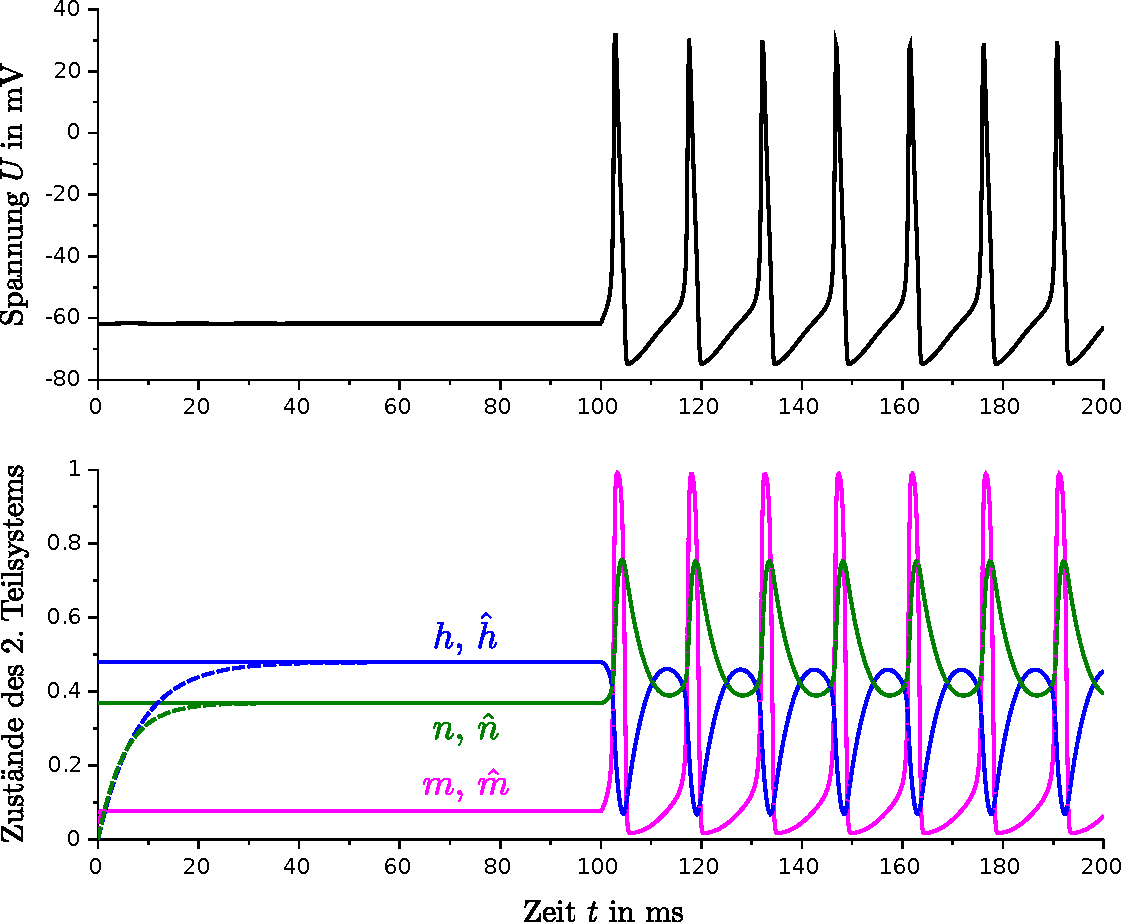
\includegraphics[width=0.95\textwidth]{Hodgkin_Sim}
\par\end{centering}
\caption{Simulierter Spannungsverlauf des Hodgkin-Huxley-Modells (oben), Trajektorien
der internen Dynamik von System und Beobachter (unten)\label{fig:hodgkin-huxley-simulation}}

\end{figure}
\end{example}

\begin{remark}
Der starke Beobachter~(\ref{eq:uio-beobachter}) lässt sich dahingehend
erweitern, dass man simultan auch eine (nicht asymptotische) Schätzung
des Eingangs erhält. Dabei nutzt man Beobachter-Filter-Kombinationen,
die in~\cite{goel2005tech,roebenack2007medjmc,roebenack2009ijss,roebenack2009ndst}
an verschiedenen Zellmodellen erprobt werden.
\end{remark}

\bibliographystyle{babalpha}
\bibliography{dynamic}

